% Options for packages loaded elsewhere
\PassOptionsToPackage{unicode}{hyperref}
\PassOptionsToPackage{hyphens}{url}
%
\documentclass[
]{article}
\usepackage{lmodern}
\usepackage{setspace}
\usepackage{amsmath}
\usepackage{ifxetex,ifluatex}
\ifnum 0\ifxetex 1\fi\ifluatex 1\fi=0 % if pdftex
  \usepackage[T1]{fontenc}
  \usepackage[utf8]{inputenc}
  \usepackage{textcomp} % provide euro and other symbols
  \usepackage{amssymb}
\else % if luatex or xetex
  \usepackage{unicode-math}
  \defaultfontfeatures{Scale=MatchLowercase}
  \defaultfontfeatures[\rmfamily]{Ligatures=TeX,Scale=1}
\fi
% Use upquote if available, for straight quotes in verbatim environments
\IfFileExists{upquote.sty}{\usepackage{upquote}}{}
\IfFileExists{microtype.sty}{% use microtype if available
  \usepackage[]{microtype}
  \UseMicrotypeSet[protrusion]{basicmath} % disable protrusion for tt fonts
}{}
\usepackage{xcolor}
\IfFileExists{xurl.sty}{\usepackage{xurl}}{} % add URL line breaks if available
\IfFileExists{bookmark.sty}{\usepackage{bookmark}}{\usepackage{hyperref}}
\hypersetup{
  pdftitle={Manuscript: Detecting differences in Size Spectra},
  pdfauthor={Justin Pomeranz1,; James R. Junker2,3; Vojsava Gjoni4; Jeff S. Wesner4},
  hidelinks,
  pdfcreator={LaTeX via pandoc}}
\urlstyle{same} % disable monospaced font for URLs
\usepackage[margin=1in]{geometry}
\usepackage{longtable,booktabs}
\usepackage{calc} % for calculating minipage widths
% Correct order of tables after \paragraph or \subparagraph
\usepackage{etoolbox}
\makeatletter
\patchcmd\longtable{\par}{\if@noskipsec\mbox{}\fi\par}{}{}
\makeatother
% Allow footnotes in longtable head/foot
\IfFileExists{footnotehyper.sty}{\usepackage{footnotehyper}}{\usepackage{footnote}}
\makesavenoteenv{longtable}
\usepackage{graphicx}
\makeatletter
\def\maxwidth{\ifdim\Gin@nat@width>\linewidth\linewidth\else\Gin@nat@width\fi}
\def\maxheight{\ifdim\Gin@nat@height>\textheight\textheight\else\Gin@nat@height\fi}
\makeatother
% Scale images if necessary, so that they will not overflow the page
% margins by default, and it is still possible to overwrite the defaults
% using explicit options in \includegraphics[width, height, ...]{}
\setkeys{Gin}{width=\maxwidth,height=\maxheight,keepaspectratio}
% Set default figure placement to htbp
\makeatletter
\def\fps@figure{htbp}
\makeatother
\setlength{\emergencystretch}{3em} % prevent overfull lines
\providecommand{\tightlist}{%
  \setlength{\itemsep}{0pt}\setlength{\parskip}{0pt}}
\setcounter{secnumdepth}{-\maxdimen} % remove section numbering
\usepackage{lineno}
\usepackage{amsmath}
\usepackage{indentfirst}
\linenumbers
\newcommand{\beginsupplement}{ \setcounter{table}{0} \renewcommand{\thetable}{S\arabic{table}} \setcounter{figure}{0} \renewcommand{\thefigure}{S\arabic{figure}}}
\ifluatex
  \usepackage{selnolig}  % disable illegal ligatures
\fi
\newlength{\cslhangindent}
\setlength{\cslhangindent}{1.5em}
\newlength{\csllabelwidth}
\setlength{\csllabelwidth}{3em}
\newenvironment{CSLReferences}[2] % #1 hanging-ident, #2 entry spacing
 {% don't indent paragraphs
  \setlength{\parindent}{0pt}
  % turn on hanging indent if param 1 is 1
  \ifodd #1 \everypar{\setlength{\hangindent}{\cslhangindent}}\ignorespaces\fi
  % set entry spacing
  \ifnum #2 > 0
  \setlength{\parskip}{#2\baselineskip}
  \fi
 }%
 {}
\usepackage{calc}
\newcommand{\CSLBlock}[1]{#1\hfill\break}
\newcommand{\CSLLeftMargin}[1]{\parbox[t]{\csllabelwidth}{#1}}
\newcommand{\CSLRightInline}[1]{\parbox[t]{\linewidth - \csllabelwidth}{#1}\break}
\newcommand{\CSLIndent}[1]{\hspace{\cslhangindent}#1}

\title{Manuscript: Detecting differences in Size Spectra}
\author{Justin Pomeranz\textsuperscript{1,*} \and James R.
Junker\textsuperscript{2,3} \and Vojsava
Gjoni\textsuperscript{4} \and Jeff S. Wesner\textsuperscript{4}}
\date{07 January, 2023}

\begin{document}
\maketitle

{
\setcounter{tocdepth}{2}
\tableofcontents
}
\setstretch{1}
\textsuperscript{1} Colorado Mesa University, Grand Junction, CO, USA\\
\textsuperscript{2} Great Lakes Research Center, Michigan Technological
University, Houghton, MI USA\\
\textsuperscript{3} Louisiana Universities Marine Consortium, Chauvin,
LA USA\\
\textsuperscript{4} Dept. of Biology, University of South Dakota,
Vermillion, SD, USA

\textsuperscript{*} Correspondence:
\href{mailto:jfpomeranz@gmail.com}{Justin Pomeranz
\textless{}\href{mailto:jfpomeranz@gmail.com}{\nolinkurl{jfpomeranz@gmail.com}}\textgreater{}}

\textbf{NOTE} I'm still working on integrating with Zotero and importing
all the necessary references (thanks Jim for the help and
instructions!). Don't worry about the \textbf{??} references in the
rendered version for now.

\hypertarget{abstract}{%
\section{Abstract}\label{abstract}}

\begin{enumerate}
\def\labelenumi{\arabic{enumi}.}
\tightlist
\item
  The distribution of body size in communities is remarkably consistent
  across habitats and taxa and can be represented by size spectra
  relationships.
\item
  Many methods have been proposed for constructing size spectra
  relationships, but recent work has shown that varied methods return
  biased estimates of relationship parameters, and different methods in
  fact are not estimating the same parameter. Despite this variability
  in estimates, it is unclear if the relative change across
  environmental gradients is consistent across methodologies. Here, we
  simulate data sets across an hypothetical environmental gradient and
  estimate the size spectra parameter (slope or exponent, depending on
  method) at each site, and, importantly, estimate the relationship of
  parameters across the hypothetical gradient. We also use two
  previously published body size datasets across an anthropogenic stress
  gradient and an environmental temperature gradient and assess how the
  conclusions of these studies would vary based on methods used.
\item
  We find that maximum likelihood methods always perform better than
  common binning methods. Additionally, the variance in estimates using
  MLE methods is markedly reduced when compared to binning methods.
\item
  The uncertainty and variation in estimates when using binning methods
  is often greater than or equal to the variation previously published
  in experimental and observational studies, bringing into question the
  effect size of previously published results. However, re-analysis of
  two previously published datasets does not markedly alter the
  conclusions reached. Further study is needed to identify how and when
  these estimates may be biased, and when the general pattern of results
  can be considered to be ``true.''
\end{enumerate}

\hypertarget{introduction}{%
\section{Introduction}\label{introduction}}

Body size distributions are a fundamental characteristic of communities.
In general, size-abundance relationships are expected to scale with the
value of -0.75 across all biological communities (Damuth 1981, 1991,
1998). This is thought to be a consequence of simple size-dependent
metabolic constraints on organisms' energy use predicted by the
metabolic theory of ecology (Nee 1991, Brown et al.~2004). The
remarkable consistency of these relationships across spatiotemporal
scales and ecosystems has led them to be recommended as a ``universal''
indicator of ecological status (Petchey and Belgrano 2010)(Petchey and
Belgrano 2010). Variation in size-abundance relationships have been
documented through space (Pomeranz 2021), time (newish Sprules papers?),
seasonality (McGarvey and Kirk), to human activities (fish abundance
with no fishing paper). Likwise, variation in size spectra relationships
have been used to explain fundamental differences in how communities are
organized. For example, external resource subsidies ``bend the rules''
and allow higher abundances of large body sizes than would be expected
(Perkins). However, recent research has shown that these results may be
an artifact of how the data were treated. Edwards et al.~(2020?)
reanalyzed a time series of marine fisheries data and found that
previously reported changes through time were actually dependent on the
methodolugy used.

Individual size distributions (ISD \emph{sensu} (White et al. 2007)),
also referred to as abundance size spectra) are one of the
size-abundance relationships commonly used. ISDs show the relationship
between the abundances of individual body size regardless of taxonomy.
Generally, there is a negative relationship between individual body size
(M) on the \emph{x}-axis and abundance (N) on the \emph{y}-axis.
Theoretical and empirical data support this relationship being described
as a simple power law with exponent \(\lambda\) in the form of
\(N \sim M^{\lambda}\), where \(\lambda = 2\). Commonly, \(N\) is the
count of body sizes grouped into bins, and \(\lambda\) is estimated as
the slope from OLS regressions of log transformed data of \(N\) and the
mid point of the body size bin \(M_{bin}\):
\(\log(N_{count}) = \lambda \log(M_{bin})\). Myriad binning methods have
been proposed, including linear and logarithmic bin widths. Likewise,
methods can rely on the absolute count in the bins as well as
normalization techniques where the count is divided by the bin width
(especially common with logarithmic binning). Alternatively, \(\lambda\)
can be estimated directly using maximum likelihood techniques.

Previous work has shown that the estimates of \(\lambda\) differ between
MLE and OLS techniques. OLS methods are particularly sensitive to
decisions made in the binning process. Simulation studies have shown
that MLE offers consistently more accurate estimates of \(\lambda\)
(White et al.~2008, Edwards et al.~2017), and reanalysis of empirical
data also indicates that the conclusions are dependent on the
methodology used Edwards et al. (2020). However, recent empirical
analysis of stream macroinvertebrate communities across the National
Ecological Observatory Network (NEON, USA) showed that while the
estimates of \(\lambda\) varied, the relative change across the
environmental gradient was consistent regardless of method used
(Pomeranz et al. 2022). While there is a growing consensus that MLE
methods offer more reliable estimates of \(\lambda\), and binning
methods result in biased estimates, it remains unclear if these biases
are consistent and systematic or stochastic, and whether or not the
relative change in ISD parameters is consistent across space and time.
In other words, if the data within a study are all treated the same,
does a relative change of OLS slope parameters of 0.1 coincide with a
relative change of MLE estimates of 0.1?

We had three primary objectives in this study: 1) how well do different
methods estimate site-specific \(\lambda\)'s? 2) Do the estimates of the
hypothetical relationship obtained from different methods agree? and 3)
Are the conclusions reached from previously published data sets
dependent on the method used?

In order to answer the first two questions, we simulate body size
observations from bounded power law distributions with varied
\(\lambda\) exponents across a hypothetical environmental gradient and
compare the results obtained using three different methodologies common
in the literature. To answer the third question, we re-analyze two
previously published data sets of stream community body sizes across a
stress and environmental gradient, respectively. We find that the MLE
method more accurately estimates the site-specific \(\lambda\) exponents
as well as the relative change in exponents across the hypothetical
gradient, as well as having smaller variation around the estimates. The
logarithmic binning methods generally perform well, but have larger
variation around the site-specific estimates. In addition, the variation
of the estimates of the hypothetical relationship obtained from the
binning methods is dependent on the value of \(\lambda\) used (under and
over estimates steep and shallow \(\lambda\), respectively).

\hypertarget{methods}{%
\section{Methods}\label{methods}}

\hypertarget{data-simulation}{%
\subsection{Data Simulation}\label{data-simulation}}

In order to investigate the performance of commonly used methods, we
simulate body size observations from a bounded power law distribution
using the inverse method, as described in (Edwards et al. 2017). Let
\(M\) be a random variable of body sizes described by the probability
density function:

\[f(M) = CM^\lambda, M_{min} \le M \le M_{max}\]

\(M_{min} = 0.0026\) and \(M_{max} = 1.2 *10^3\). These values are based
on empirical body sizes of stream benthic communities reported in
(Pomeranz et al. 2022). Our results are not dependent on the range of
body sizes, and we show the results of other body size ranges in the
supplemental information.

\hypertarget{site-specific-lambda-estimates}{%
\subsection{\texorpdfstring{Site-specific \(\lambda\)
estimates}{Site-specific \textbackslash lambda estimates}}\label{site-specific-lambda-estimates}}

We sampled \(n = 1000\) body sizes from distributions described by five
different \(\lambda\)'s: (-1.5, -1.75, -2.00, -2.25, -2.5). The values
of \(\lambda\) describe how quickly the abundance of large body sizes
decline within a community, e.g., a value of -1.5 means there would be a
relatively high number of large body sizes (shallow) whereas a value of
-2.5 means there would be relatively very few large body sizes (steep).
We used three different methods (described below) to estimate the value
of \(\lambda\). We repeated this process 1000 times (reps) and plot the
distribution of values obtained for each method.

\hypertarget{estimation-of-size-spectra-parameter-lambda}{%
\subsection{\texorpdfstring{Estimation of Size spectra parameter
\(\lambda\)}{Estimation of Size spectra parameter \textbackslash lambda}}\label{estimation-of-size-spectra-parameter-lambda}}

For each sample of \(M\) and each of the 1000 replicates, we estimated
the exponent \(\lambda\) directly using MLE methods modified from the
the \texttt{sizeSpectra} package (Edwards et al.~2020). Throughout the
manuscript, these estimates are referred to as MLE.

\hypertarget{equal-logarithmic-bins-elbn}{%
\subsubsection{Equal Logarithmic Bins:
ELBn}\label{equal-logarithmic-bins-elbn}}

In addition, we use two common binning methods to estimate the OLS slope
parameter in log-log space. It is important to note that the binning
methods are estimating a slope (\(\beta_{1}\)) from an OLS regression
analysis, and not \(\lambda\) directly. However, in the interest of
clarity, we will refer to all estimates as \(\lambda\) regardless of the
method used, and reserve the term \(\beta_{env}\) to refer to the
estimate of the size spectra relationships across the hypothetical
environmental gradient.

For the first binning method, we created 6 equal logarithmic bins
covering the range of body sizes. This method has been used extensively
in previous studies. For example see Dossena et al. (2012). In the
present study, the count in each bin was normalized by dividing by the
bin width to account for the unequal bin sizes. The process of
normalizing shifts the estimate by -1. In other words, an un-normalized
estimate of -0.75 would result in an estimate of -1.75 when normalizing
the data (Sprules and Barth 2015 pp. Edwards2018, Pomeranz2022).
Throughout the manuscript, the normalized equal logarithmic binning
method will be referred to as ELBn.

\hypertarget{log2-bins-nas}{%
\subsubsection{\texorpdfstring{Log\textsubscript{2} Bins:
NAS}{Log2 Bins: NAS}}\label{log2-bins-nas}}

The second method was similar to ELBn, but bins of Log\textsubscript{2}
widths are used. The number of bins is dependent on the size ranges
present in the data. When working with empirical data with different
size ranges this can alter the number of bins per site. However, since
the data here were simulated from a known size range, the number of bins
for each site is identical. The count in each bin is normalized in the
same way. This method has been used {[}Jennings and Blanchard (2004),
Jennings et al. (2002), Sprules and Barth (2015), Pomeranz et al.
(2019a); McGarvey and Kirk (2018)) and is referred to as the Normalized
Abundance Spectrum (NAS).

For the two binning methods, simple OLS regression were conducted in the
form \(Log_{10}(N) = \beta_0 + \beta_1 * Log_{10}(M)\). Where
\(\beta_{1}\) is considered to be the \(\lambda_{estimate}\).

\hypertarget{variation-in-lambda-across-a-gradient}{%
\subsection{\texorpdfstring{Variation in \(\lambda\) Across a
Gradient}{Variation in \textbackslash lambda Across a Gradient}}\label{variation-in-lambda-across-a-gradient}}

\hypertarget{hypothetical-relationshiop-of--0.5}{%
\subsubsection{Hypothetical relationshiop of
-0.5}\label{hypothetical-relationshiop-of--0.5}}

Previous work has investigated the biases in \(\lambda\) estimates when
using different methods White et al. (2007). However, the focus of the
present work is to investigate biases when estimating the relationship
parameters across an environmental gradient.

To do this, we again sampled body sizes from distributions described by
five different \(\lambda\)'s. However, because the estimates from the
binning methods varied depending on the value of \(\lambda\) (see
results), we chose three different ``windows'' of lambda values. The
three windows were steep
(\(\lambda = [-1.50,~ -1.75,~ -2.00,~ -2.25, -2.50]\)), medium
(\(\lambda = [-1.00,~ -1.25,~ -1.50,~ -1.75,~ -2.00]\)), and shallow
((\(\lambda = [-0.50,~ -0.75,~ -1.00,~ -1.25,~ -1.50]\)).

\textbf{NOTE} This MS seems to be getting long. Possibly present
``medium'' window in main results, and include other windows in SI

Each sample of body sizes from different \(\lambda\) values was assumed
to come from a community across a hypothetical environmental gradient
\(X\). Values of \(X\) for each community are uniformly distributed from
-1 to 1 (site-specific x-values: \((-1.0, -0.5, 0, 0.5, 1.0)\). For each
\(\lambda\) ``window,'' the relative change in \(\lambda\) values
(\(\beta_{env}\)) across the gradient is equal to -0.5, such that our
model is:

\textbf{JEFF} Is this correct? for some reason this seems wrong to me.

\[\beta_{env} = Norm(\alpha -0.5X,~\sigma)\]

We repeated the data simulation 1000 times (reps). The main results
presented here were not dependent on the range of \emph{x}-values or the
number of sites (supplemental information).

\hypertarget{varying-hypothetical-relationship}{%
\subsubsection{Varying Hypothetical
Relationship}\label{varying-hypothetical-relationship}}

Finally, we also varied the relationship (\(\beta_{env}\)) across the
hypothetical gradient. We tested \(\beta_{env}\) values of 0, -0.25, and
-0.5 by sampling 5 body sizes communities uniformly distributed across
the following sets of \(\lambda\) values: {[}-1.5{]}, {[}-1.25,
-1.75{]}, {[}-1, -2{]}.

\hypertarget{estimation-of-relationship-across-gradient-beta_env}{%
\subsection{\texorpdfstring{Estimation of relationship across gradient,
\(\beta_{env}\)}{Estimation of relationship across gradient, \textbackslash beta\_\{env\}}}\label{estimation-of-relationship-across-gradient-beta_env}}

For each simulation replicate and size spectra method, we estimated how
the size spectra parameters varied across the hypothetical gradient. We
did this by performing simple OLS regression of the
\(\lambda_{estimate}\) across the hypothetical gradient (\(X\)):

\[\lambda_{estimate} = \beta_0 + \beta_{env} * X\]

The distribution of the relationship coefficient, \(\beta_{env}\), were
plotted compared to the known relationship.

\hypertarget{empirical-data}{%
\subsection{Empirical Data}\label{empirical-data}}

We re-analyze two data sets of benthic macroinvertebrate communities
from stream habitats across two different gradients. In the first,
quantitative macroinvertebrate samples were collected from streams
across an acid mine drainage (AMD) stress gradient. Details of the
sample collection and processing can be found in (Pomeranz et al.
2019a). Briefly, all individuals from each sample were identified to the
lowest practical taxonomic unit and body lengths were measured using
image processing software from photos taken with a camera mounted to a
dissecting microscope. Body mass was estimated using taxon-specific
published length weight regressions.

The second data set was from the wadeable stream sites of the National
Ecological Observatory Network (National Ecological Observatory Network
(NEON) 2022). NEON stream sites are located across a wide temperature
gradient in the United States, from Puerto Rico to Alaska. Quantitative
macroinvertebrate samples were collected using the most appropriate
method based on the local habitat. All individuals were identified and
had their body lengths measured, and body mass was estimated using
published length weight regressions. This data has been analyzed
previously using size spectra methods as described in (Pomeranz et al.
2022). Detailed methods of the sampling collection and data processing
methods can be found on the NEON website
({[}\url{https://www.neonscience.org/data-collection/macroinvertebrates}{]},
or macroinvertebrate DPI pubs). Coefficient estimates (\(\pm\) 1
standard deviation) are compared across methods. This allows us to
determine whether or not the main results would differ depending on the
method used.

\hypertarget{data-availabity}{%
\subsection{Data Availabity}\label{data-availabity}}

The data used in this manuscript is already publicly available (Pomeranz
et al. 2019b) data dryad DOI
\url{https://datadryad.org/stash/dataset/doi:10.5061/dryad.v6g985s},
(National Ecological Observatory Network (NEON) 2022). R Scripts to
reproduce the full simulation and analysis are available at:
({[}\url{https://github.com/Jpomz/detecting-spectra-differences}{]}).

\hypertarget{results}{%
\section{Results}\label{results}}

\hypertarget{lambda-estimates}{%
\section{\texorpdfstring{\(\lambda\)
estimates}{\textbackslash lambda estimates}}\label{lambda-estimates}}

There was considerable variation in the \(\lambda\) estimate across
methodologies (Figure 1). The distribution of estimates from the MLE
method was almost always symmetrical and centered at the known value of
\(\lambda\) (Figure 1, blue distribution and dashed line). The
distribution of estimates from the binning methods were generally wider,
and sometimes showed assymetrical distributions.

\begin{figure}
\centering
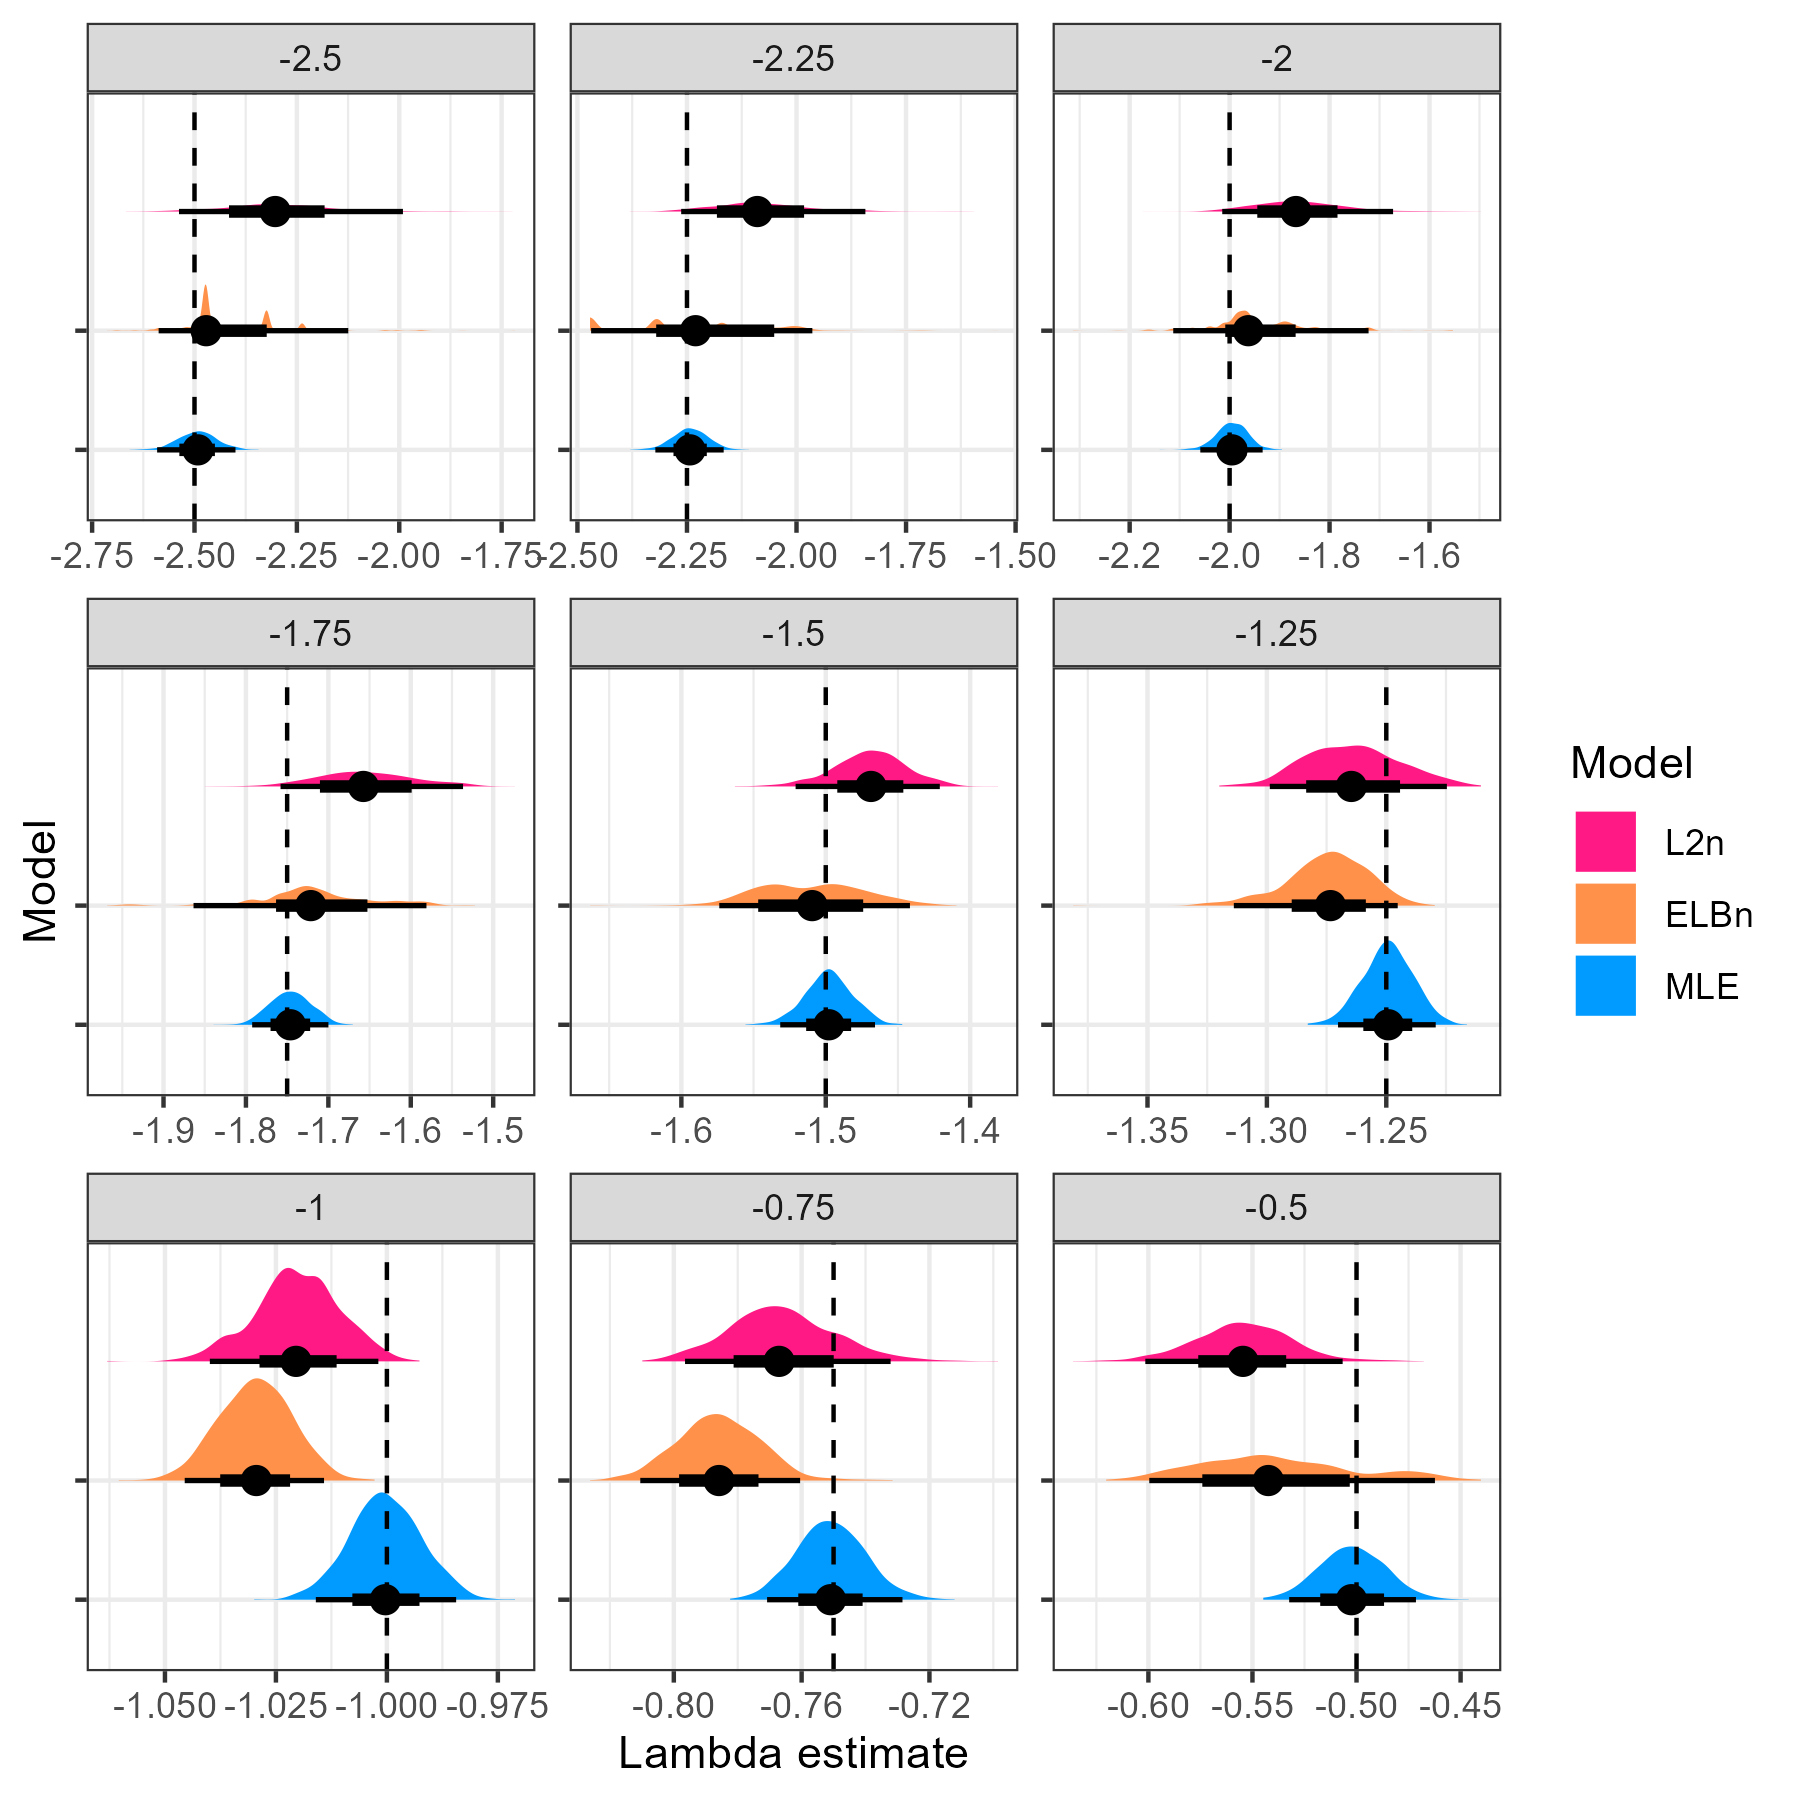
\includegraphics{figures/est_lambda_est_b_density.png}
\caption{Figure 1. Distribution of Lambda estimates by method (color)
from random samples of body sizes from bounded power law distributions
with varying exponents (-2.5, -0.5). The figure is facetted by the known
lambda parameter (facet title) and is also shown as the dashed line in
each facet. Note that the x-axis varies in each facet.}
\end{figure}

Furthermore, the binning methods systematically over estimated steep
size spectra relationships (\(\lambda = ~\sim-2.5~to-1.5\), Figure 2),
and slightly underestimated shallow size spectra relationships
(\(\lambda = ~\sim-0.5\)). This finding was more pronounced in the NAS
method compared with the ELBn method.

\begin{figure}
\centering
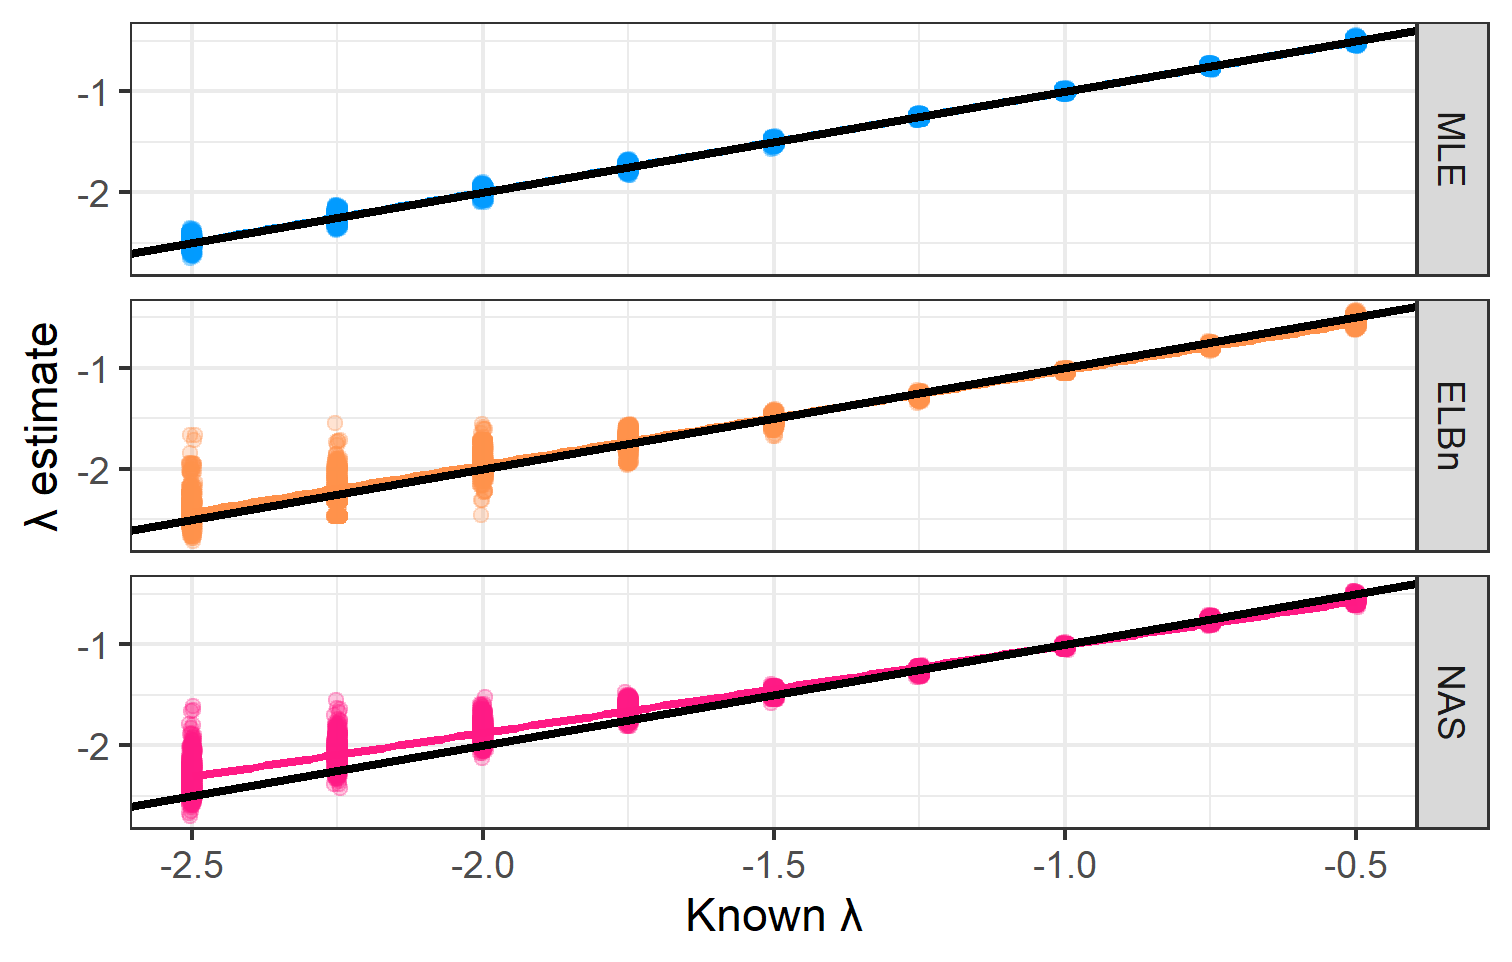
\includegraphics{figures/known_est_b_line.png}
\caption{Figure 2. Plot of the known and estimated lambda from different
methods (color). The dashed line is the 1:1 line, and almost perfectly
matches the MLE (Blue) estimate. The two binning method cross the 1:1
line, meaning they systematically underestimate shallow lambdas, and
over estimate steeper lambdas.}
\end{figure}

\hypertarget{relationship-across-the-hypothetical-environmental-gradient}{%
\subsection{Relationship across the hypothetical environmental
gradient}\label{relationship-across-the-hypothetical-environmental-gradient}}

\hypertarget{lambda-windows}{%
\subsubsection{\texorpdfstring{\(\lambda\)
``windows''}{\textbackslash lambda ``windows''}}\label{lambda-windows}}

Because of the different performance of the two binning methods at steep
and shallow values of lambdas, we first investigated how well the
methods capture a known relationship of \(\beta_{env} = -0.5\) across a
hypothetical environmental gradient. The lambda ``windows'' are steep
(-2.5, -1.5), medium (-2, -1) and shallow (-1.5, -0.5).

\begin{figure}
\centering
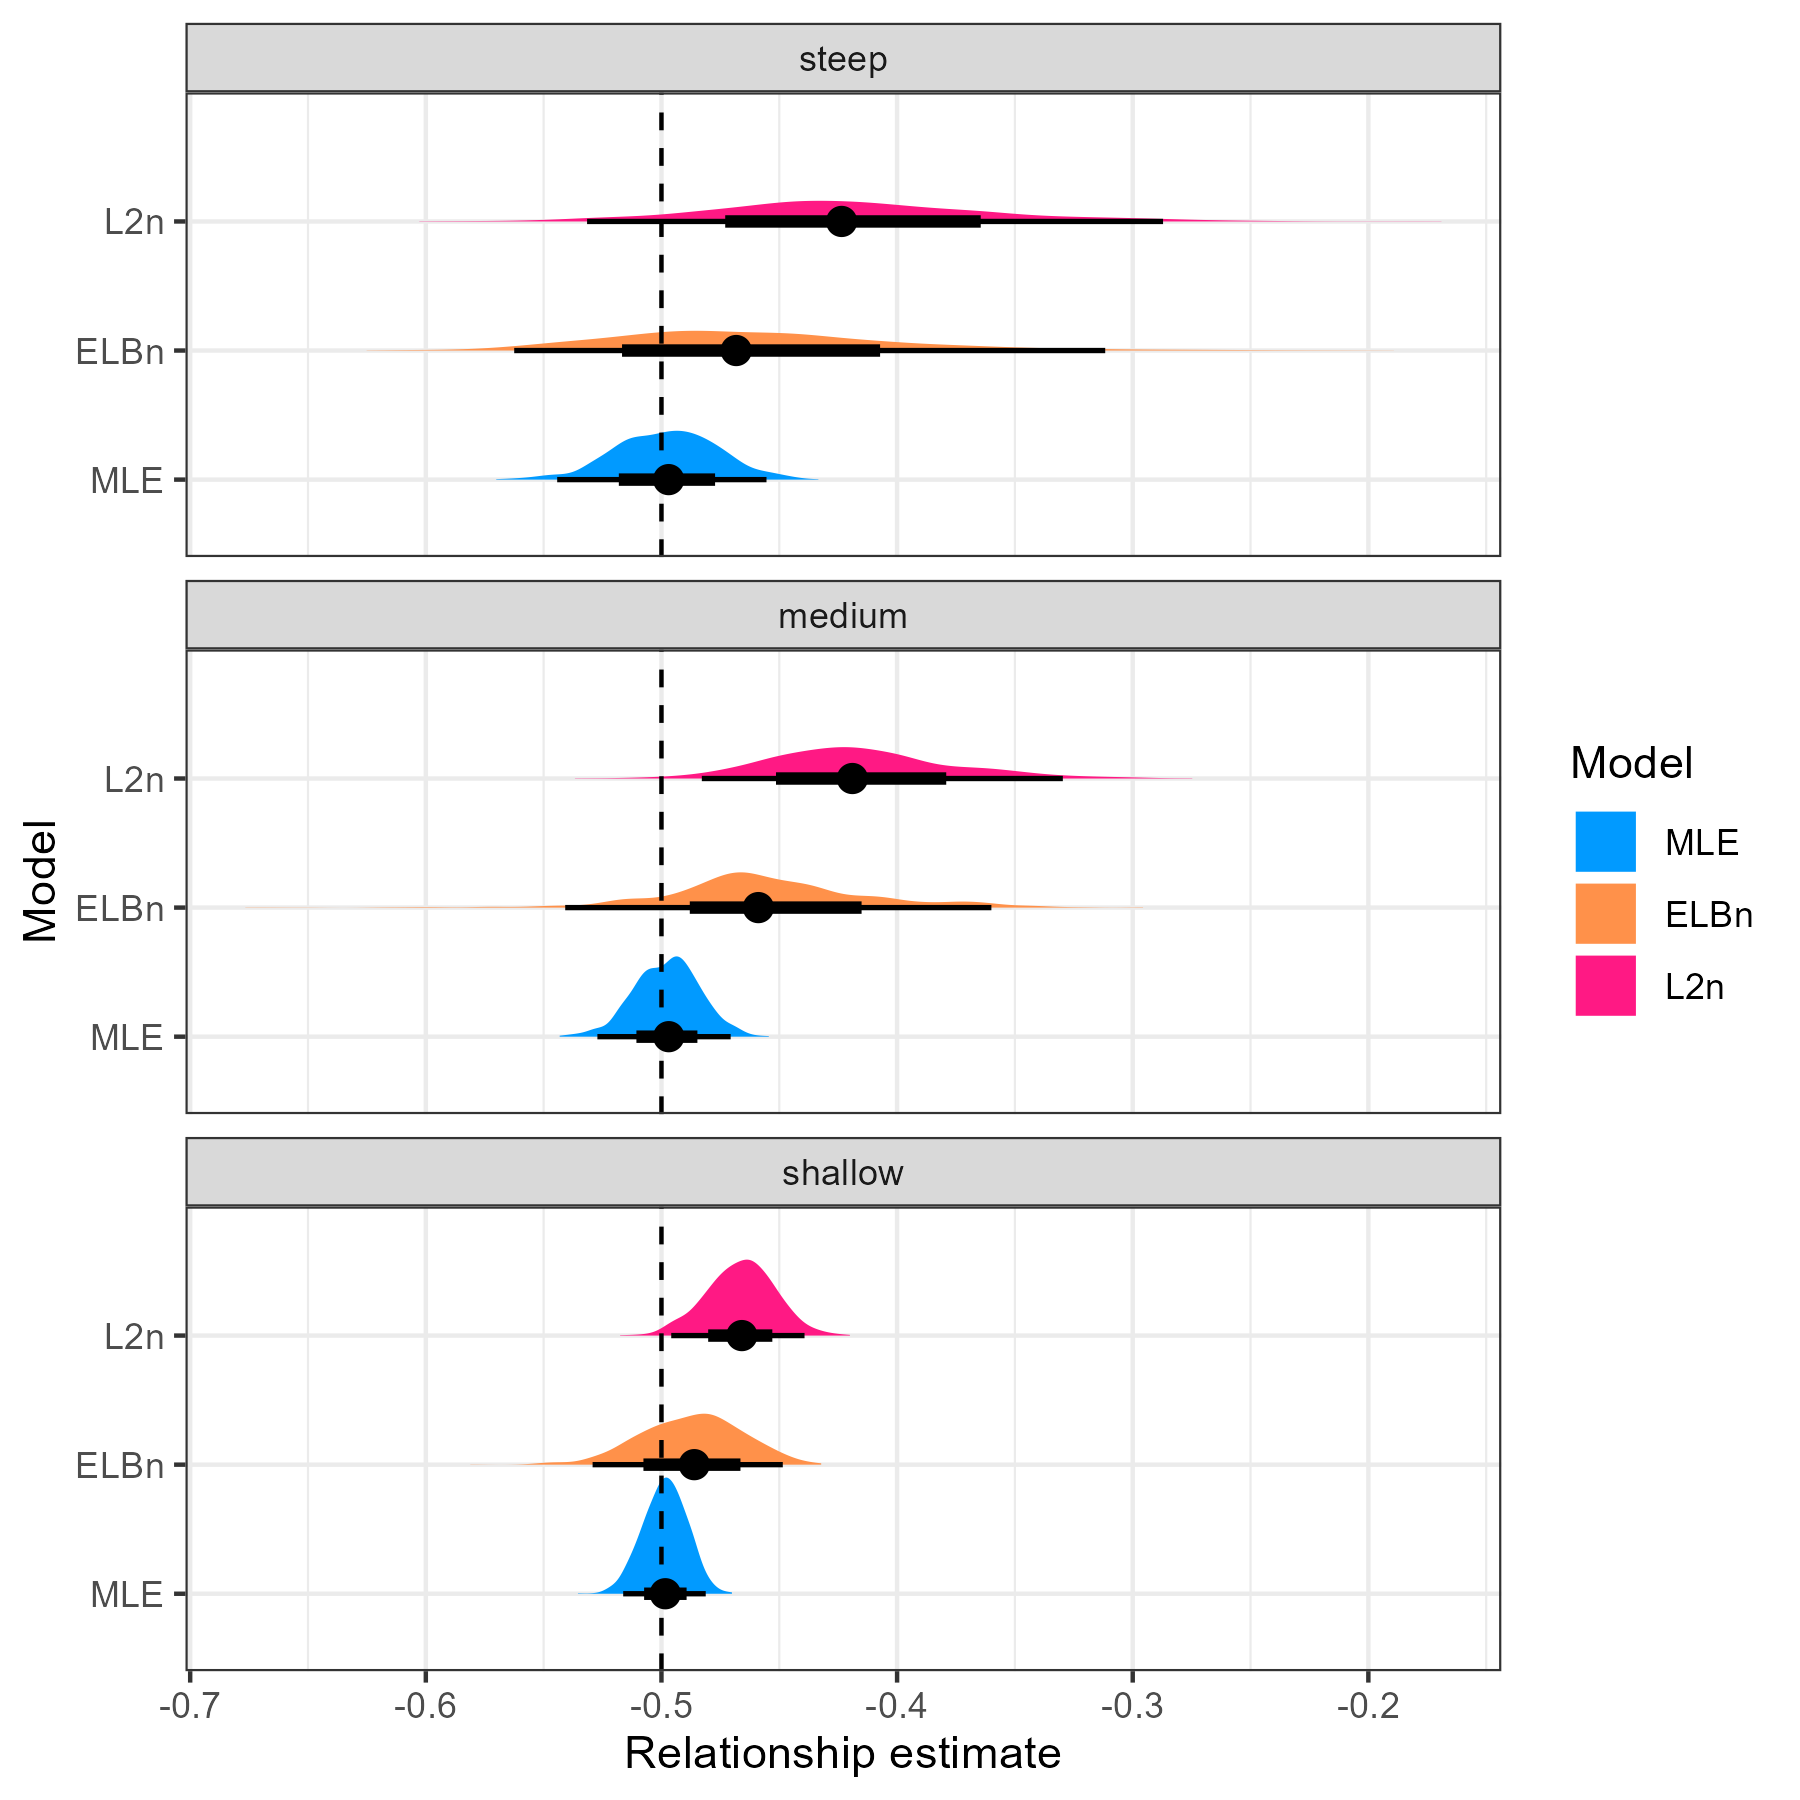
\includegraphics{figures/lambda_angle_plot.png}
\caption{Figure 3. Distribution of relationship estimates
(\(beta_{env}\)) in three different ``windows'' of lambda values. The
dashed vertical line is the known relationship value of -0.5.}
\end{figure}

The distribution of relationship estimates from the MLE method (Figure
3, blue) is approximately centered at the known relationship value in
each of the ``windows.'' The distribution for the MLE estimate is widest
in the ``steep'' window, but is still markedly narrower than the binning
methods. In addition to having much wider distributions, the binning
methods systematically overestimate the known relationship.

\hypertarget{varying-the-known-relationship}{%
\subsubsection{Varying the Known
Relationship}\label{varying-the-known-relationship}}

Finally, we were interested in finding if the three methods performed
differently with varying values of the known relationship. Here, we
present estimates from each method when the known relationship
(\(\beta_{env}\)) across the hypothetical gradient was -0.5, -0.25, and
0, respectively (Figure 4).

\begin{figure}
\centering
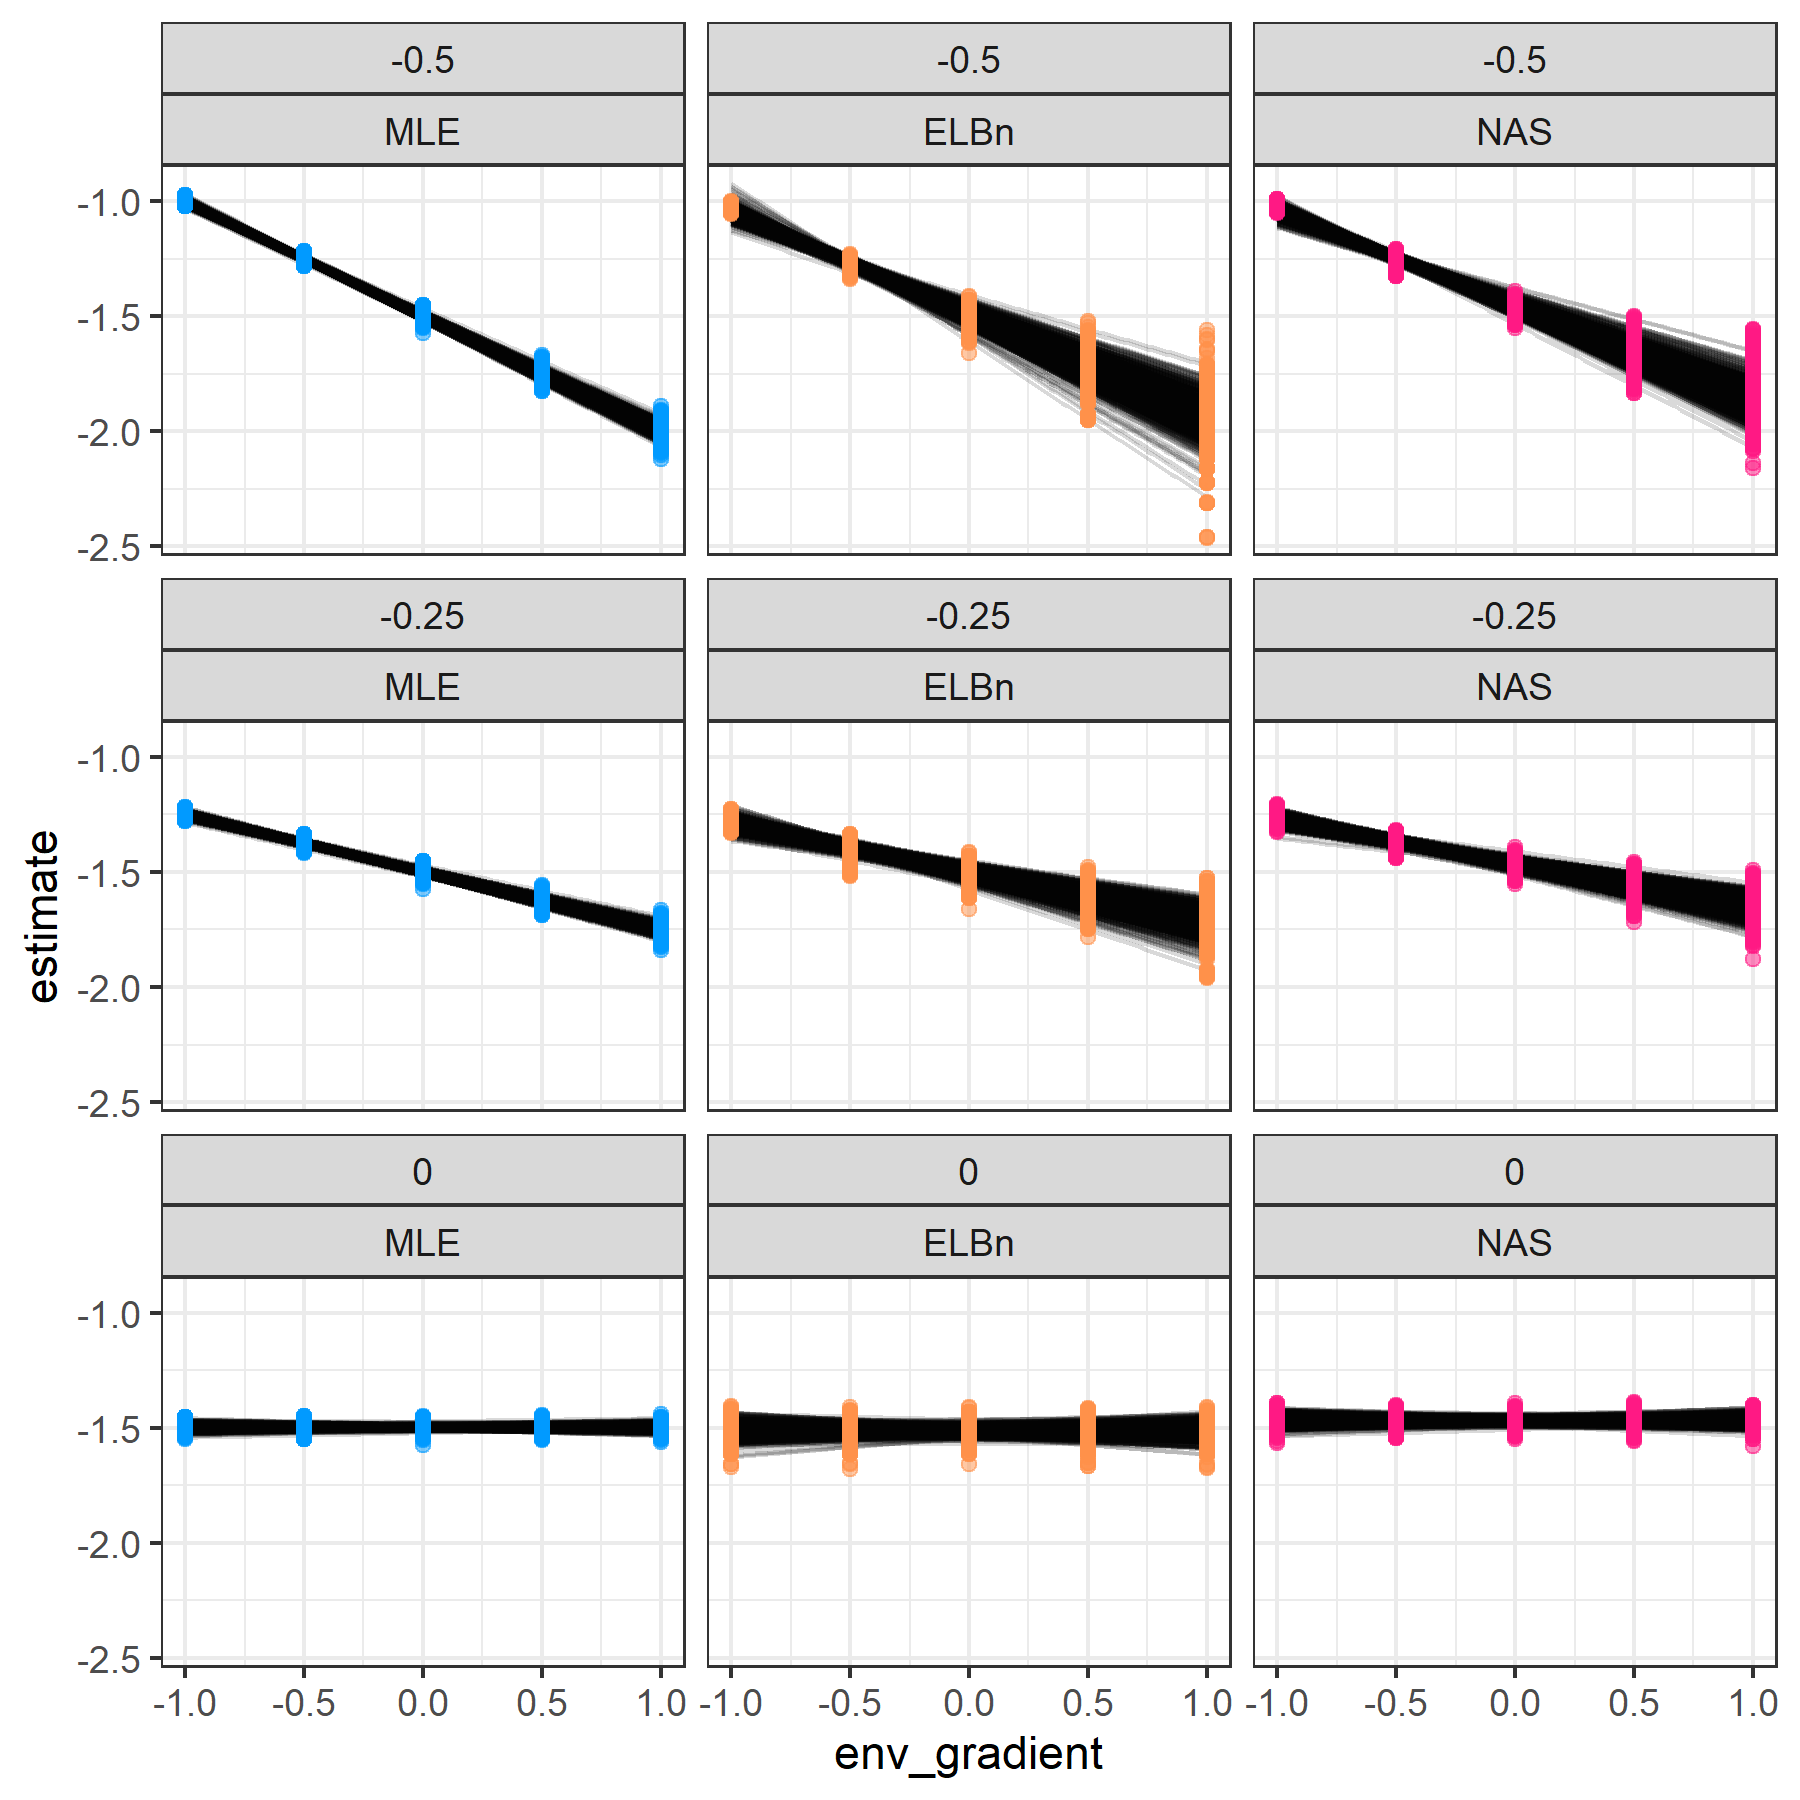
\includegraphics{figures/vary_beta_plot.png}
\caption{Figure 4. Individual regressions for each rep (N = 1000) and
method (columns) for three different known relationship values (rows):
0, 0.25, and 0.5}
\end{figure}

Likewise, we also present the distribution of the \(\beta_{env}\)
relationship estimates (Figure 5). All the methods perform similarly and
reasonably well when no relationship is present. The performance of the
binning methods declines (center of distributions), with relationships
being systematically over estimated. Likewise, the width of the
distributions increases with stronger relationships across a
hypothetical gradient. However, the distribution of estimates from the
MLE method is nearly always centered at the known value, and has
relatively narrow distributions.

\begin{figure}
\centering
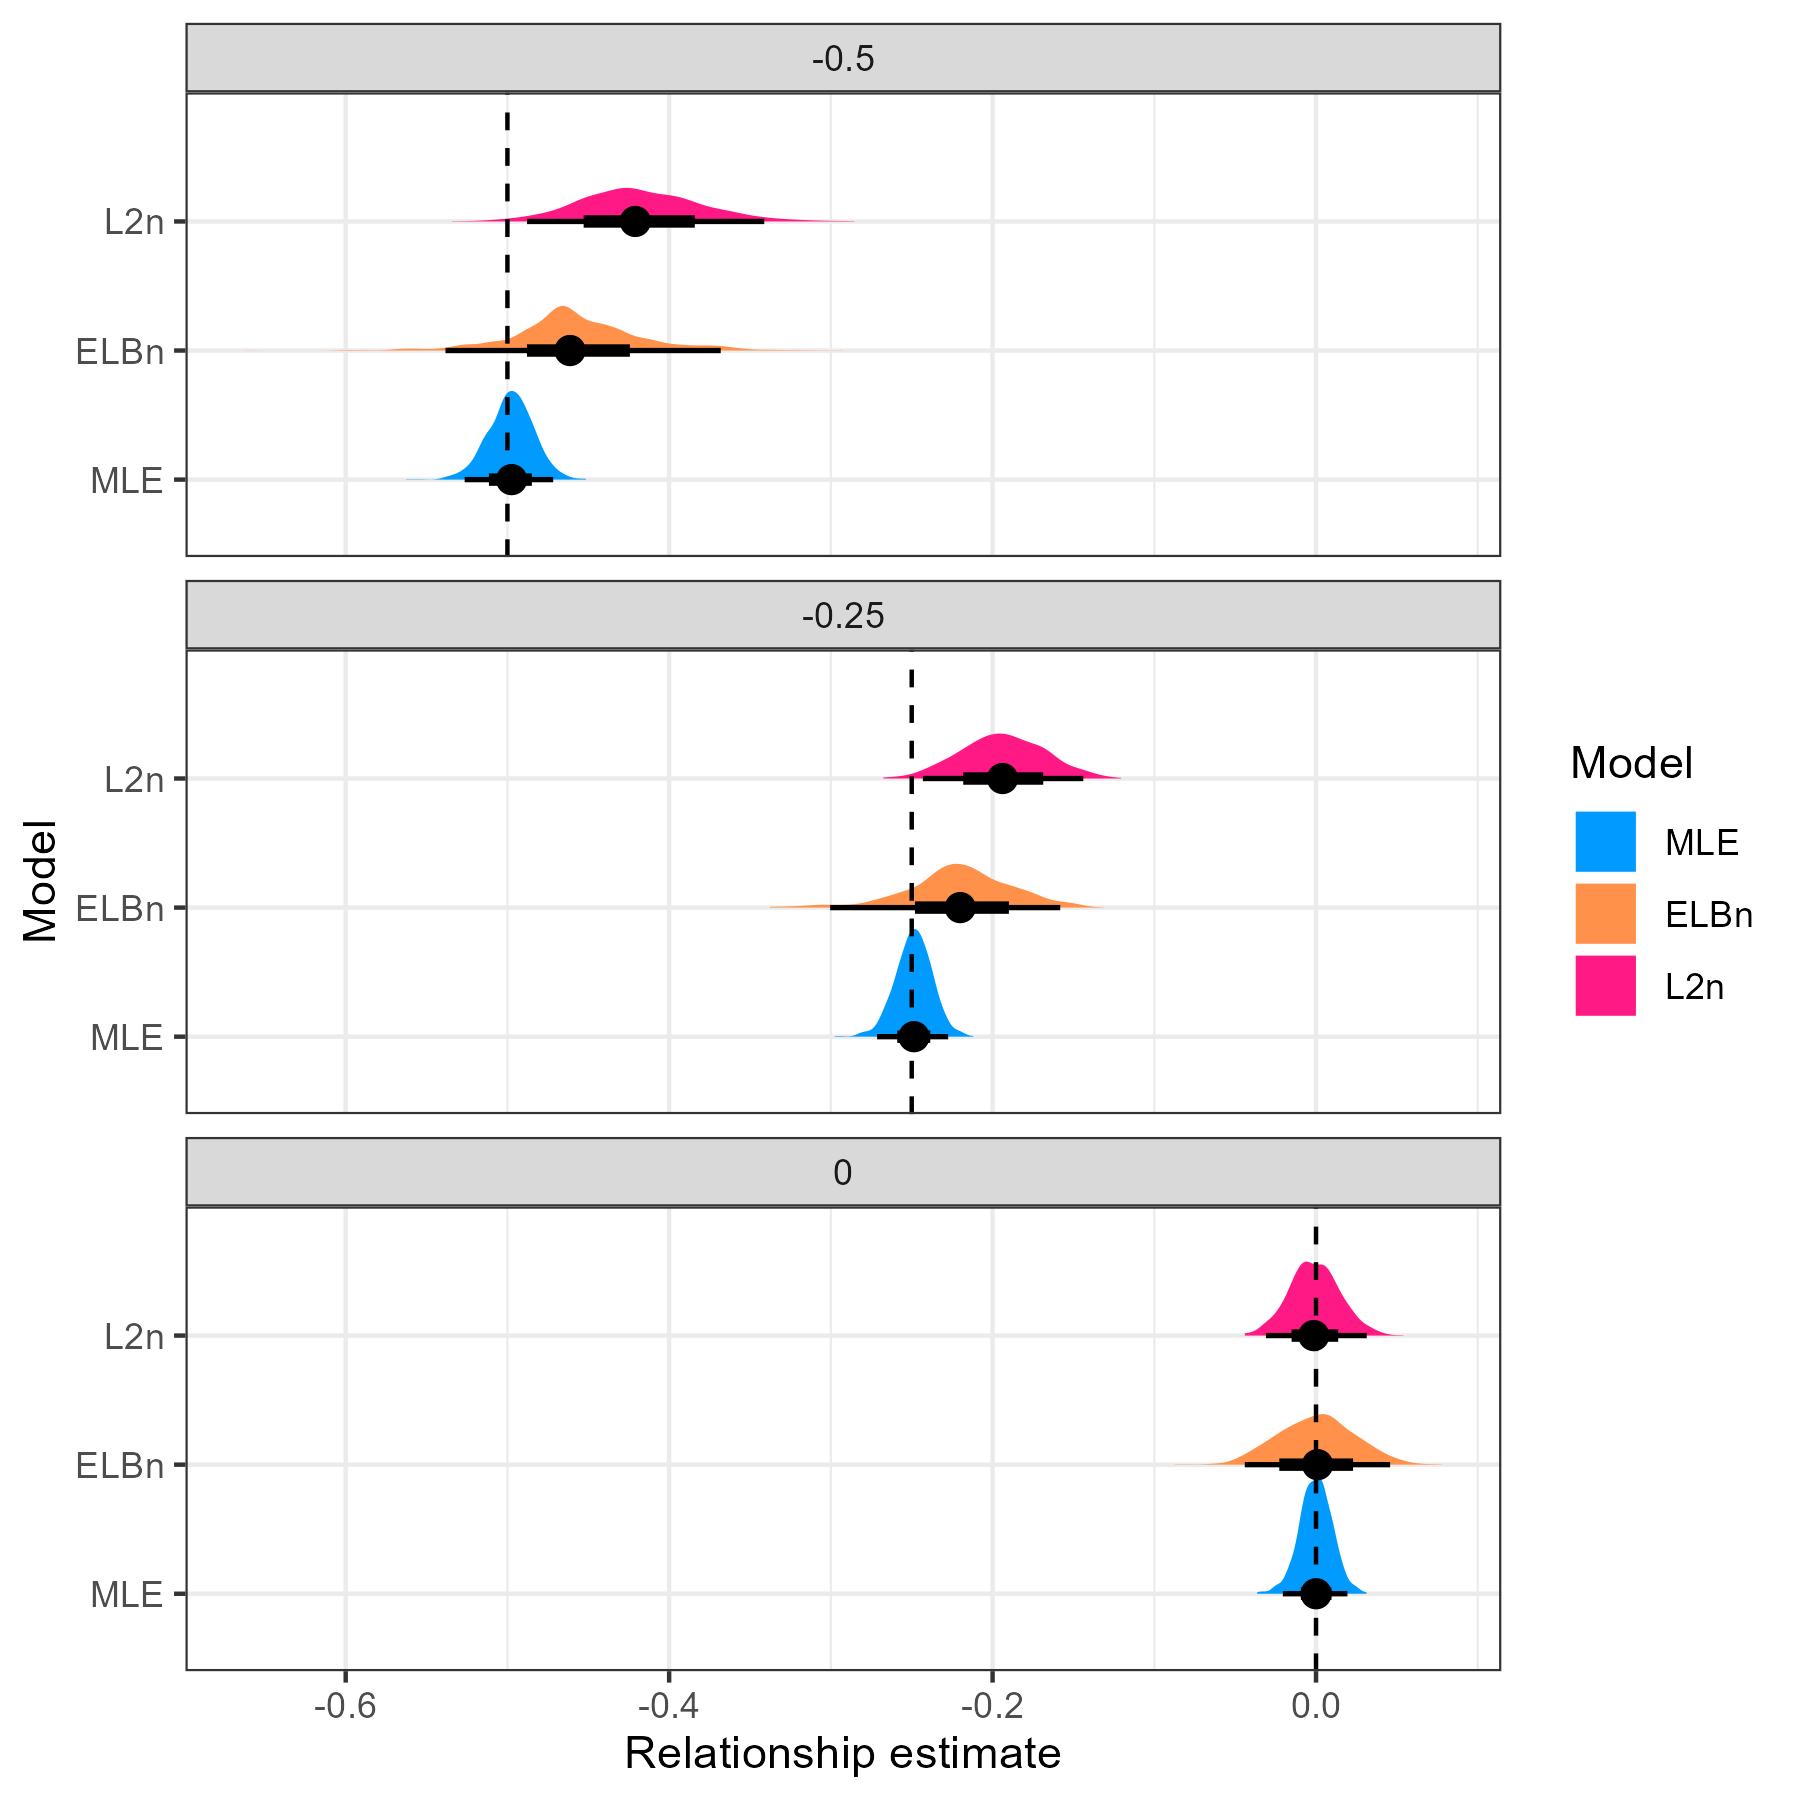
\includegraphics{figures/vary_beta_density_plot.png}
\caption{Figure 5. Distribution of relationship estimates (beta\_1) when
estimating from different known relationships}
\end{figure}

\hypertarget{empirical-data-1}{%
\subsection{Empirical data}\label{empirical-data-1}}

For both empirical data sets, the direction and magnitude of change
(i.e.~\(\beta_1\) coefficients) are generally in agreement. Size spectra
parameters consistently increase (become flatter) in the AMD data (Fig.
6A). However, the magnitude of the change across the AMD gradient is
weakest using the MLE method, and the width of the estimates (\(\pm\) 1
SD) is larger in the binning methods, particularly the ELBn method (Fig.
6B). Likewise, the size spectra parameters consistently increase (become
steeper) with increasing temperature across the NEON sites (Fig. 6C).
The magnitude of the relationships is weakest in the MLE method,
although the uncertainty around the estimates are similar (Fig. 6D).

\newpage

\begin{figure}
\centering
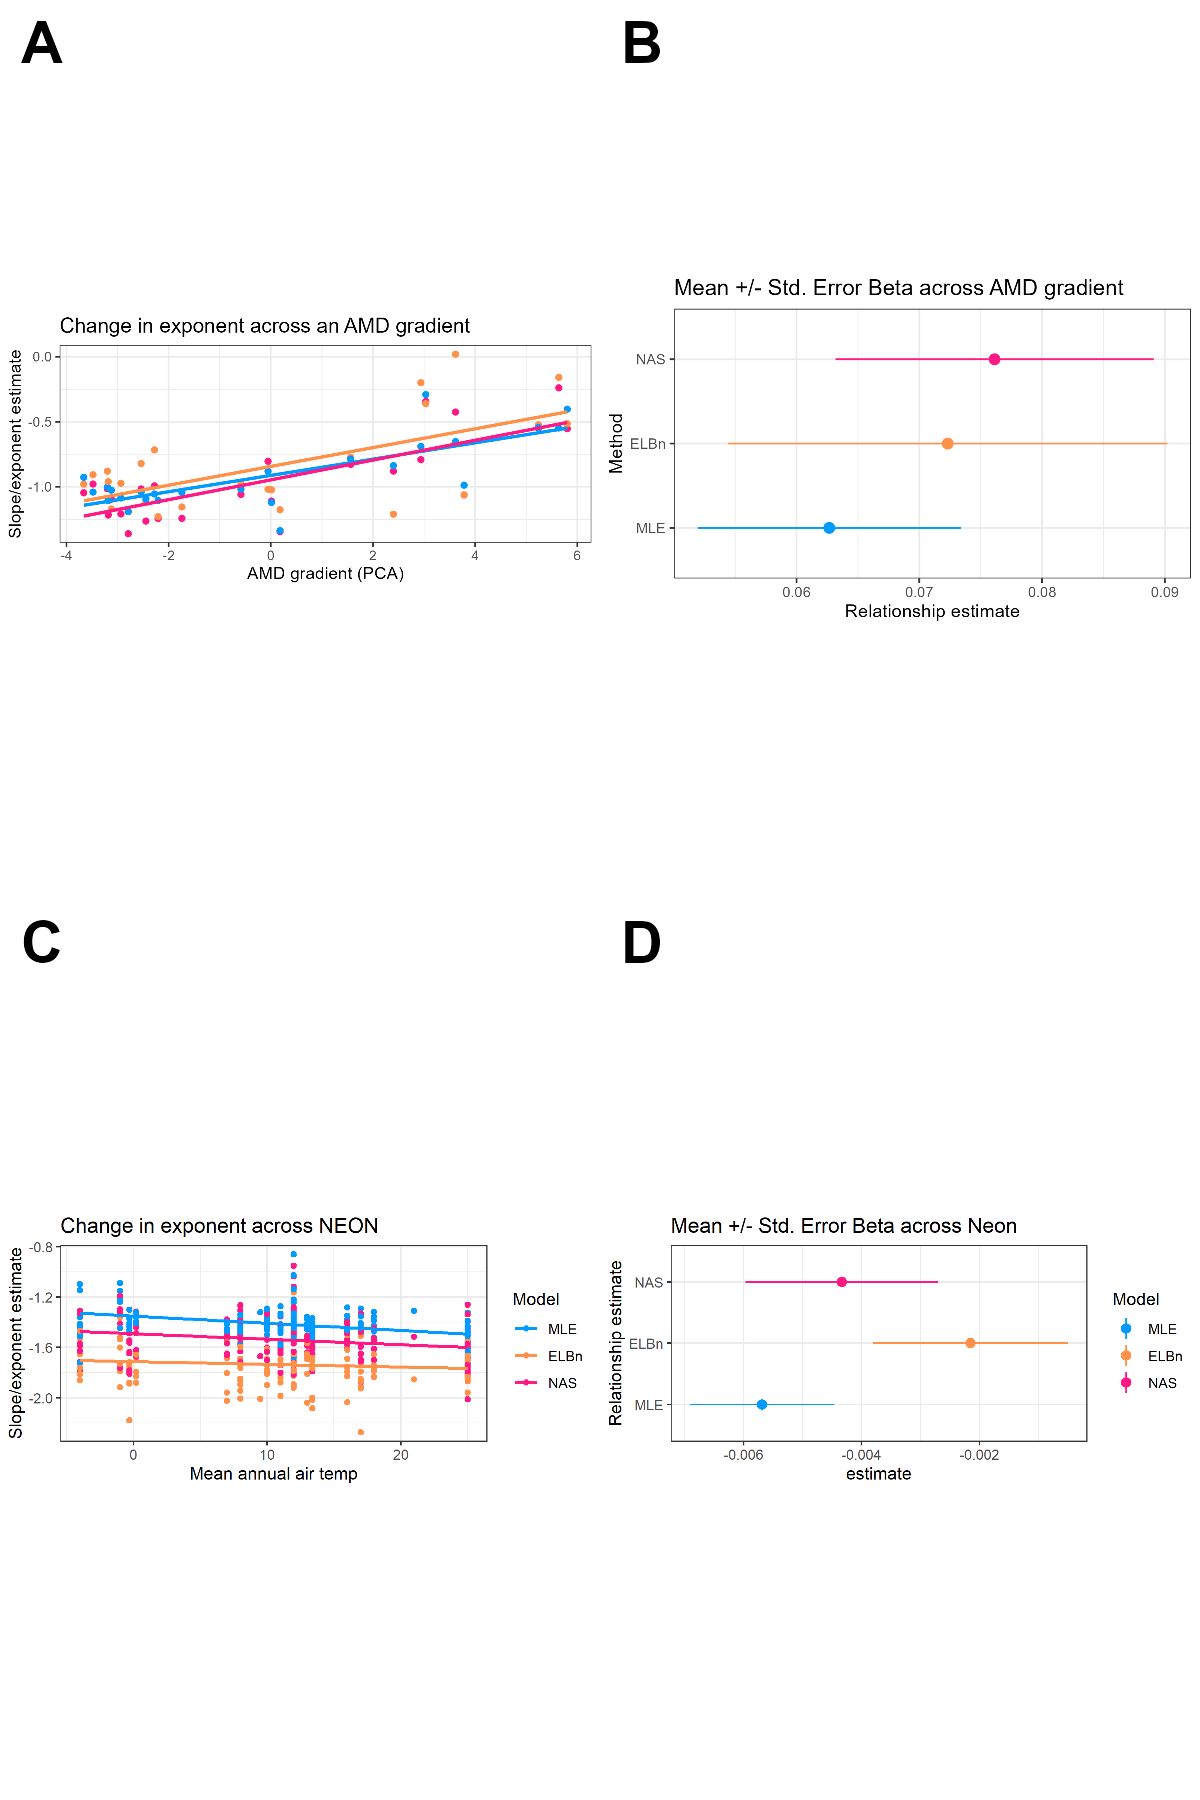
\includegraphics{figures/empirical_combined.png}
\caption{Figure 6. of empirical data estimates. All of the methods
estimate the same sign of the relationship, but the estimates from the
binning methods are generally greater than the MLE estimates.
\textbf{NOTE} I need to re-plot these in ggplot and and stitch together.
Currently stitching pre-made png files, I think that's why it looks so
funky.}
\end{figure}

\newpage

The \(\beta_1\) coefficient estimates for the AMD data are all positive
and of relatively similar magnitudes across methods. The MLE estimate
has the smallest magnitude and SD (0.063 \(\pm\) 0.011 SD), The ELBn
method is slightly larger and has a wider SD : (0.072 \(\pm\) 0.018).
Finally, the NAS method has the largest estimate and an intermediate
standard deviation (0.076 \(\pm\) 0.013). The range of the gradient in
the AMD data is relatively small (9.5), but the absolute change in the
size spectra parameter (\(\lambda\)) across the AMD gradient vary by
\textasciitilde0.13 units depending on the method used (range of
absolute change: 0.59 to 0.72).

Similar to the AMD results, the \(\beta_1\) coefficient estimates for
the NEON data are all negative and have similar magnitudes across
methods. The MLE estimate is once again the smallest (-0.006 \(\pm\)
0.001 SD). The NAS and ELBn methods are larger at -0.004 \(\pm\) 0.002,
and -0.002 \(\pm\) 0.002, respectively. Although the estimates are
similar and have a small magnitude, the range of the gradient in this
data is larger (\textasciitilde30\(\circ\)C), meaning that the absolute
change in \(\lambda\) estimates varies by 0.11 units depending on the
methods used (range of absolute change across gradient: 0.06 to 0.17).

\hypertarget{discussion}{%
\section{Discussion}\label{discussion}}

The relationship between body size and abundance has been extensively
studied in a wide range of taxa inhabiting both terrestrial and aquatic
ecosystems (reviewed by White et al. (2007)). Empirical patterns are
remarkably consistent, and can be explained by the metabolic theory of
Ecology (Brown et al. 2004). Measuring parameters describing the decline
in abundance with increasing body size in communities is being done with
increasing frequency across ecology. Previous work has investigated the
accuracy and inherent biases associated with different estimation
methods. However, how these inaccuracies and biases compound across
environmental gradients remains uncertain, making it difficult to detect
variation in size spectra parameters across environmental gradients with
confidence. Here, we sampled body sizes from known distributions with
varying parameters (\(\lambda\)) and estimated the coefficient of the
relationship (\(\beta_{env}\)) across a hypothetical gradient in order
to assess how the results would vary depending on the method used.
Likewise, we compared how the interpretation of previously published
results could change depending on the methodology used to estimate the
relationship.

Generally, the estimate of the size spectra parameter from the MLE
method was always closer to the known \(\lambda\) value, regardless of
how steep or shallow the \(\lambda\) exponent was. This is in agreement
with Edwards et at. (2017) which found that the MLE estimate more
consistently recovered known \(\lambda\) values ranging from -2.5 to
-0.5. We further this work by discovering that the magnitude of the
error associated with the two binning methods increases as the
\(\lambda\) value moves away from \(\sim\) -1.

It is unsurprising that all methods performed less well in estimating
steep values of \(\lambda\) (i.e., -2.5). The rapid decline of large
body sizes makes it unlikely to sample any individuals with a large body
size. Furthermore, the binning methods inherently ``lose'' data by
aggregating individual observations into a single bin.

Likewise, the MLE method also resulted in the most accurate
\(\beta_{env}\) estimates for the hypothetical relationship in simulated
data regardless of the \(\lambda\) ``window'' investigated. Furthermore,
the variation around the estimate was always smallest with the MLE
method. However, the variation in the MLE estimate did increase with
steeper \(\lambda\) ``windows.'' This is not surprising, however because
steep relationships like this make it very unlikely to sample the
largest body sizes, and capturing the ``true'' relationships without the
full range of body sizes present is more difficult (Edwards et
al.~2017). Despite this, the MLE method is nearly always the best option
to use, likely because all the data are used in the analysis.

Binning methods are easy to use and interpret, which most likely
accounts for their wide use in ecological studies. However, aggregating
individuals into logarithmic bins removes a large source of the
variation within the data by collapsing body size variation into a
single value within each bin. For example, all individuals placed into a
bin that ranges from 2-4 grams of mass are all treated as having a mass
of 3 grams, the midpoint of that bin. Likewise, a single abundance value
is taken for this bin, despite that fact that there is almost certainly
variation in the abundance of individuals that weigh \textasciitilde2,
\textasciitilde3, or \textasciitilde4 grams. By homogenizing the data in
this way, it seems that binning methods will always produce noisier
results than MLE from the binning process alone, since binning is akin
to deleting information that the model could otherwise use. One of the
benefits of using MLE is that all data points are retained for use
within the model.

The variation in estimated relationships across the empirical datasets
varied by \textasciitilde0.1 units depending on the method used. At
first glance this may not appear to be a concerning magnitude of
variation. However, when one considers the range of variation reported
in many seminal works on variation in size spectra relationships is
\textasciitilde0.1-0.2 (SI Table \emph{xx}), it becomes clear how
important an error in estimates of this magnitude is.

Despite the differences in magnitude of the empirical relationship
coefficients, they were generally in the correct direction and of a
similar magnitude. This suggests that previously reported significant
changes in size spectra parameters across environmental gradients and in
experimental manipulations are plausible. Given that all of the data
within a study is treated identically, the over all change in size
spectra parameters is likely reasonable. However, the biases and
inconsistencies in relationship estimates presented here suggest that it
would be difficult if not impossible to directly compare the relative
changes across different published studies which use different methods.
However, the relatively systematic error of \(\lambda\) estimates across
known exponents suggests that it may be possible to correct previous
estimates onto the same scale (Figure 2).

Despite this possibility, publication of individual body size data with
future studies of size spectra relationships would greatly aid in our
ability to generalize changes to this fundamental aspect of community
organization across spatiotemporal scales and in response to
environmental conditions.

\hypertarget{concluding-remarks}{%
\subsection{Concluding Remarks}\label{concluding-remarks}}

The MLE method outperformed both of the binning methods under nearly any
measure. With the publication of the \emph{sizespectra} package (2017),
producing MLE estimates of size spectra parameters is a relatively easy
task. Therefore, we recommend using this in all future studies of size
spectra relationships.

We reiterate the recommendations of (2017) to estimate size spectra
relationships using MLE methods due to their superior performance in
nearly every context. Furthermore, we strongly encourage authors to
publish individual size data whenever possible. This will allow for the
consistent re-analysis of existing data sets as methodologies develop
and improve. This will aid in the ability for size spectra work to be
synthesized between research groups and across scales.

\newpage

\hypertarget{references}{%
\section{References}\label{references}}

\hypertarget{refs}{}
\begin{CSLReferences}{1}{0}
\leavevmode\hypertarget{ref-Brown1995}{}%
Brown, J. H. 1995. Macroecology. {University of Chicago Press},
{Chicago, IL}.

\leavevmode\hypertarget{ref-Brown2004}{}%
Brown, J. H., J. F. Gillooly, A. P. Allen, V. M. Savage, and G. B. West.
2004. Toward a metabolic theory of ecology. Ecology 85:1771--1789.

\leavevmode\hypertarget{ref-dossenaWarmingAltersCommunity2012}{}%
Dossena, M., G. Yvon-Durocher, J. Grey, J. M. Montoya, D. M. Perkins, M.
Trimmer, and G. Woodward. 2012. Warming alters community size structure
and ecosystem functioning. Proceedings of the Royal Society B
279:3011--3019.

\leavevmode\hypertarget{ref-edwards2020}{}%
Edwards, A. M., J. Robinson, J. Blanchard, J. Baum, and M. Plank. 2020.
Accounting for the bin structure of data removes bias when fitting size
spectra. Marine Ecology Progress Series 636:19--33.

\leavevmode\hypertarget{ref-Edwards2017}{}%
Edwards, A. M., J. Robinson, M. Plank, J. Baum, and J. Blanchard. 2017.
Testing and recommending methods for fitting size spectra to data.
Methods in Ecology and Evolution 8:57--67.

\leavevmode\hypertarget{ref-jennings2004}{}%
Jennings, S., and J. L. Blanchard. 2004. Fish abundance with no fishing:
Predictions based on macroecological theory. Journal of Animal Ecology
73:632--642.

\leavevmode\hypertarget{ref-Jennings2002}{}%
Jennings, S., K. J. Warr, and S. Mackinson. 2002. Use of size-based
production and stable isotope analyses to predict trophic transfer
efficiencies and predator-prey body mass ratios in food webs. Marine
Ecology Progress Series 240:11--20.

\leavevmode\hypertarget{ref-martinez2016}{}%
Martínez, A., A. Larrañaga, A. Miguélez, G. Yvon-Durocher, and J. Pozo.
2016. Land use change affects macroinvertebrate community size spectrum
in streams: The case of {Pinus} radiata plantations. Freshwater Biology
61:69--79.

\leavevmode\hypertarget{ref-mcgarveySeasonalComparisonCommunitylevel2018}{}%
McGarvey, D. J., and A. J. Kirk. 2018. Seasonal comparison of
community-level size-spectra in southern coalfield streams of {West
Virginia} ({USA}). Hydrobiologia 809:65--77.

\leavevmode\hypertarget{ref-NEON_Inverts2022}{}%
National Ecological Observatory Network (NEON). 2022. Macroinvertebrate
collection ({DP1}.20120.001). {National Ecological Observatory Network
(NEON)}.

\leavevmode\hypertarget{ref-Perkins2018}{}%
Perkins, D. M., I. Durance, F. K. Edwards, J. Grey, A. G. Hildrew, M.
Jackson, J. I. Jones, R. B. Lauridsen, K. Layer-Dobra, M. S. A.
Thompson, and G. Woodward. 2018. Bending the rules: Exploitation of
allochthonous resources by a top-predator modifies size-abundance
scaling in stream food webs. Ecology Letters.

\leavevmode\hypertarget{ref-Petchey2010}{}%
Petchey, O. L., and A. Belgrano. 2010. Body-size distributions and
size-spectra: Universal indicators of ecological status? Biology Letters
6:434--437.

\leavevmode\hypertarget{ref-Pomeranz2022}{}%
Pomeranz, J. P. F., J. R. Junker, and J. S. Wesner. 2022. Individual
size distributions across {North American} streams vary with local
temperature. Global Change Biology 28:848--858.

\leavevmode\hypertarget{ref-pomeranzAnthropogenicMiningAlters2019}{}%
Pomeranz, J. P. F., H. J. Warburton, and J. S. Harding. 2019a.
Anthropogenic mining alters macroinvertebrate size spectra in streams.
Freshwater Biology 64:81--92.

\leavevmode\hypertarget{ref-Pomeranz2019}{}%
Pomeranz, J. P. F., H. J. Warburton, and J. S. Harding. 2019b. Data
from: {Anthropogenic} mining alters macroinvertebrate size spectra in
streams. {Dryad}.

\leavevmode\hypertarget{ref-sprulesSurfingBiomassSize2015}{}%
Sprules, and Barth. 2015. Surfing the biomass size spectrum: Some
remarks on history, theory, and application. Canadian Journal of
Fisheries and Aquatic Sciences 73:477--495.

\leavevmode\hypertarget{ref-white2008}{}%
White, E. P., B. J. Enquist, and J. L. Green. 2008. On estimating the
exponent of power-law frequency distributions. Ecology 89:905--912.

\leavevmode\hypertarget{ref-White2007}{}%
White, E. P., S. K. M. Ernest, A. J. Kerkhoff, and B. J. Enquist. 2007.
Relationships between body size and abundance in ecology. Trends in
Ecology \& Evolution 22:323--330.

\end{CSLReferences}

\newpage

\hypertarget{supplementary-material}{%
\section*{Supplementary material}\label{supplementary-material}}
\addcontentsline{toc}{section}{Supplementary material}

\beginsupplement

\hypertarget{lambda-and-relationship-estimates}{%
\section{\texorpdfstring{\(\lambda\) and relationship
estimates}{\textbackslash lambda and relationship estimates}}\label{lambda-and-relationship-estimates}}

In the main analysis, we simulate body size data from bounded power law
distributions while varying the \(\lambda\) exponent which describes the
distribution. For the results presented in the main text, we held the
number of sites at 5, scaled the environmental gradient from -1 to 1,
and set the minimum and maximum body sizes to \(0.0026\) and
\(1.2 *10^3\) respectively. Here, we plot the results of varying the
number of sites (3, 10), increasing the scale of the environmental
gradient (-100 to 100) and decreasing the range of body sizes (min = 1,
max = 100). Generally, the results reported in the main manuscript are
robust to changing these parameters: the MLE estimate is nearly always
closer to the known parameters, and the variation in these estimates is
usually smaller than the binning methods.

\hypertarget{varying-number-of-sites}{%
\subsection{Varying number of sites}\label{varying-number-of-sites}}

\hypertarget{sites}{%
\subsubsection{10 sites}\label{sites}}

\begin{figure}
\centering
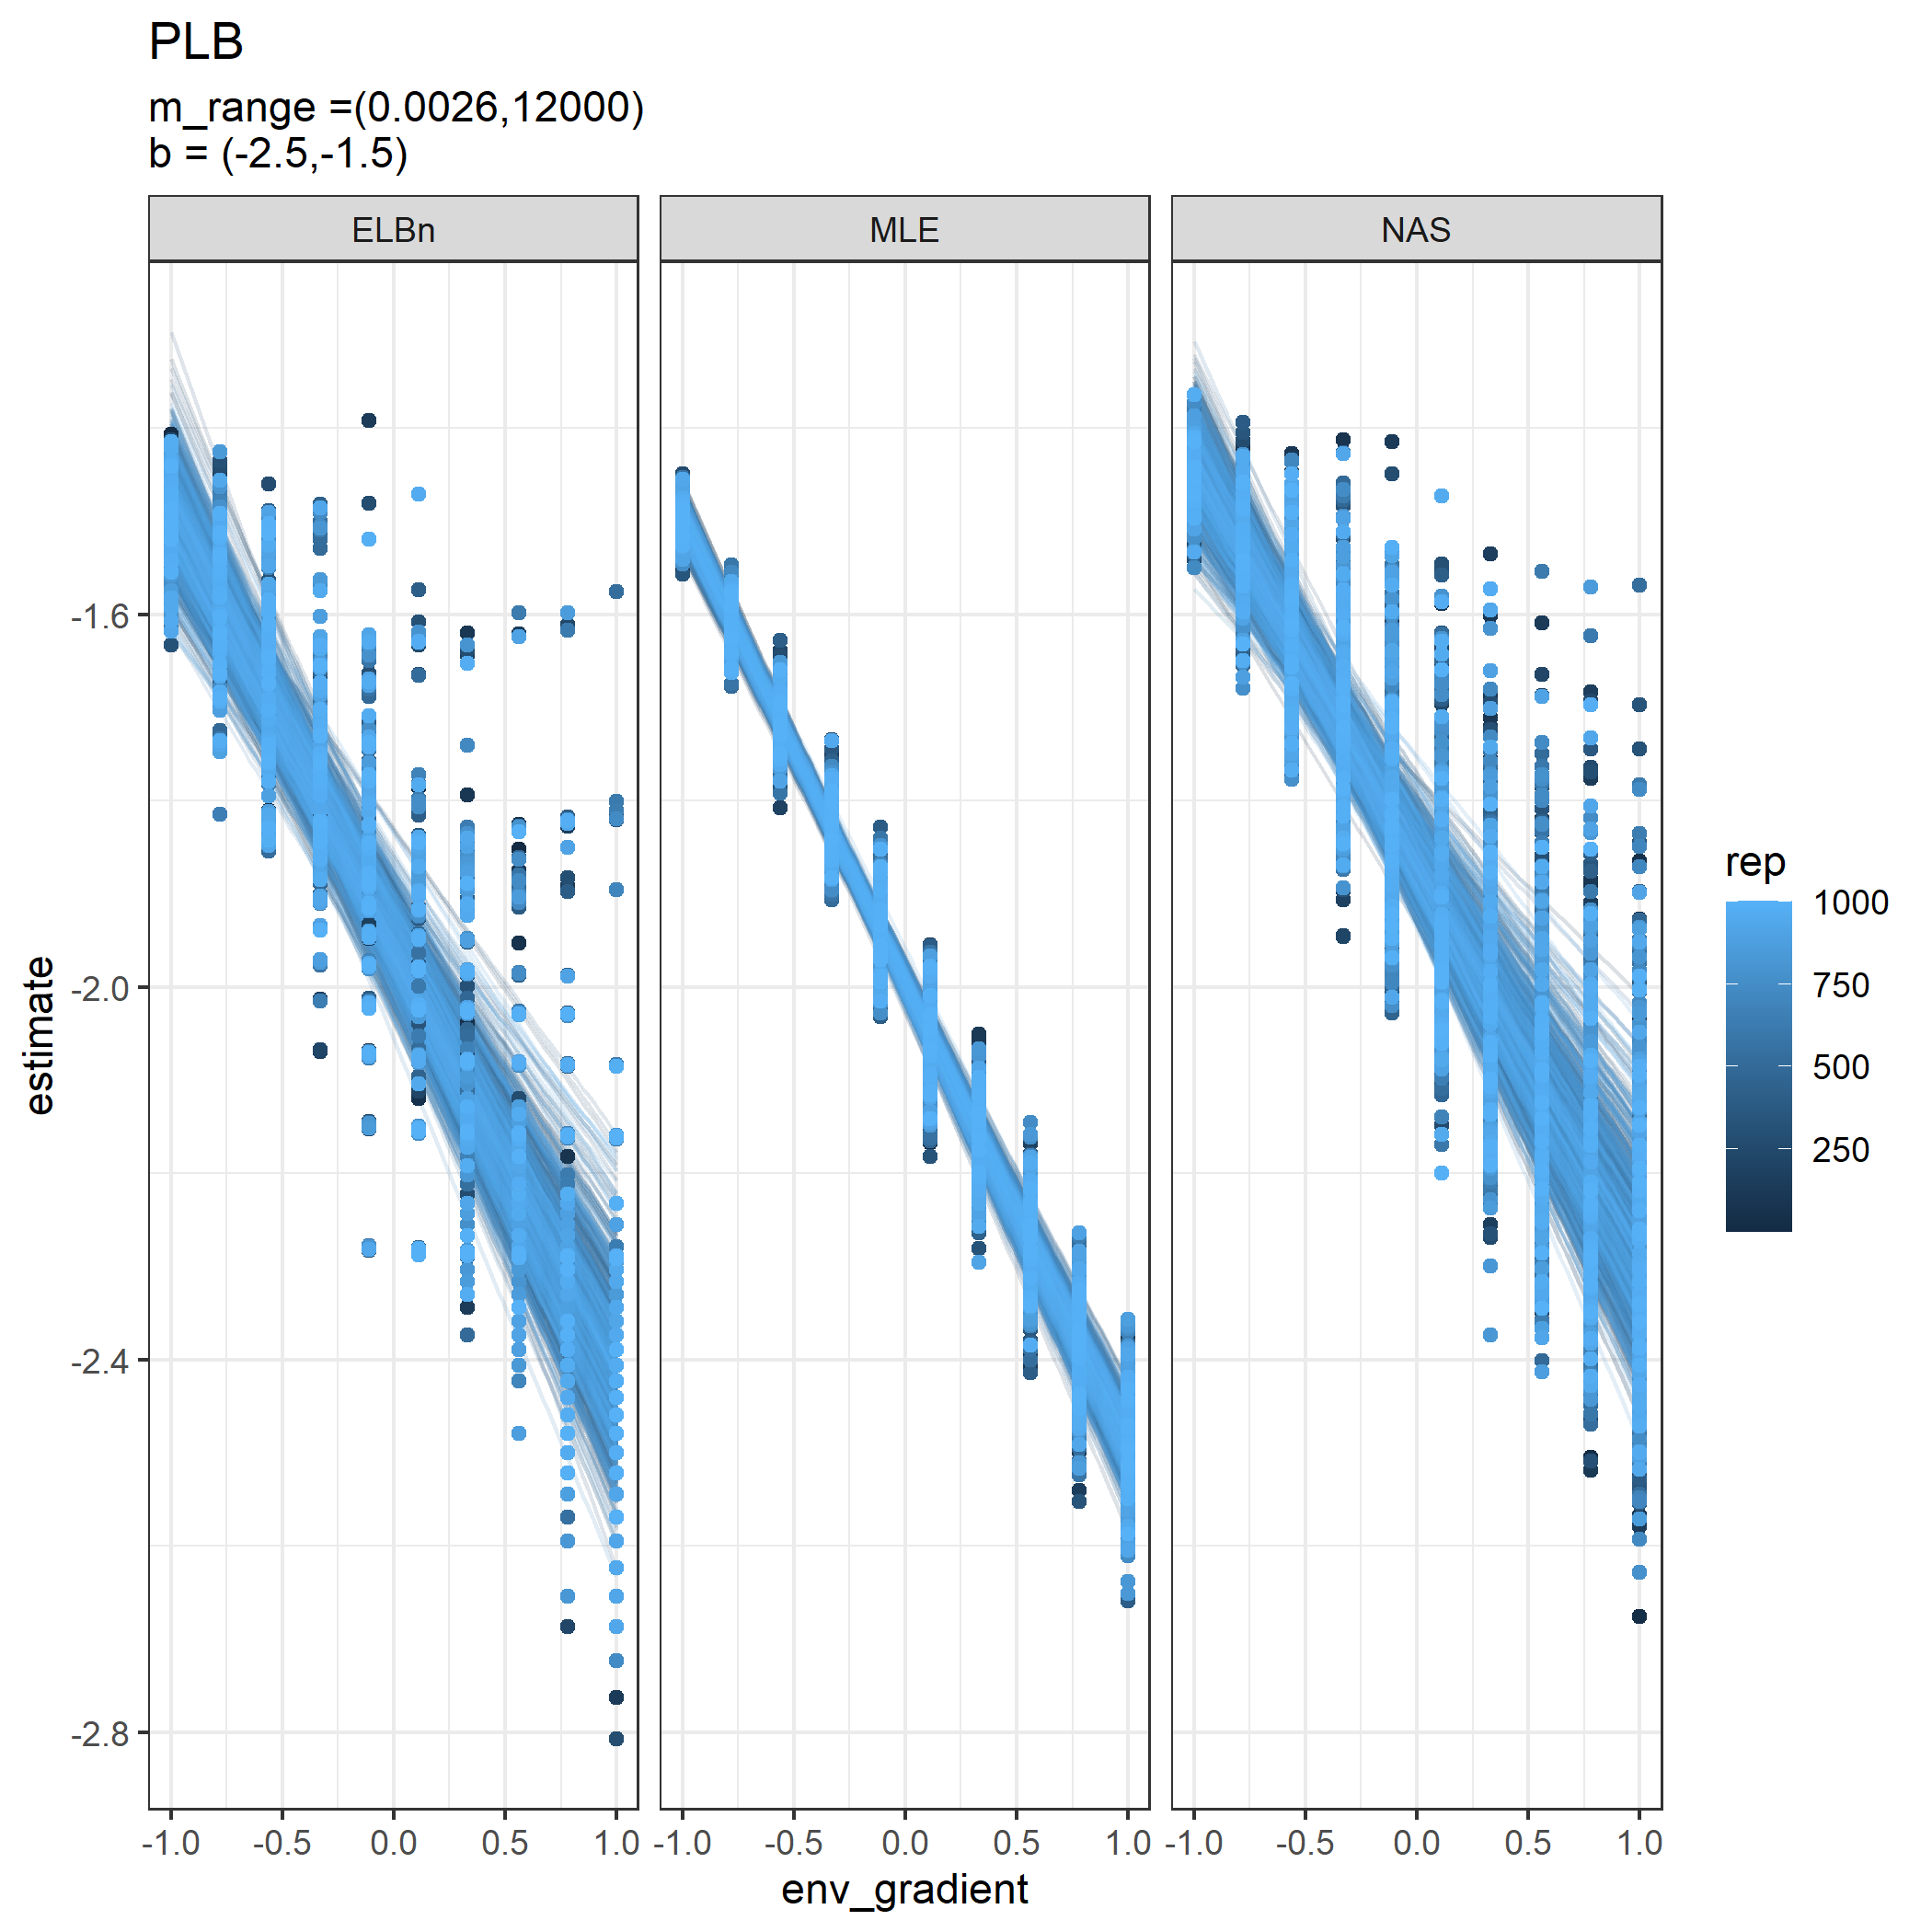
\includegraphics{figures/PLB_10_sites_main.png}
\caption{Individual regressions for ten sites across a hypothetical
gradient with a known relationship of 0.5. All other parameters are the
same as in the main analysis}
\end{figure}

\newpage

\begin{figure}
\centering
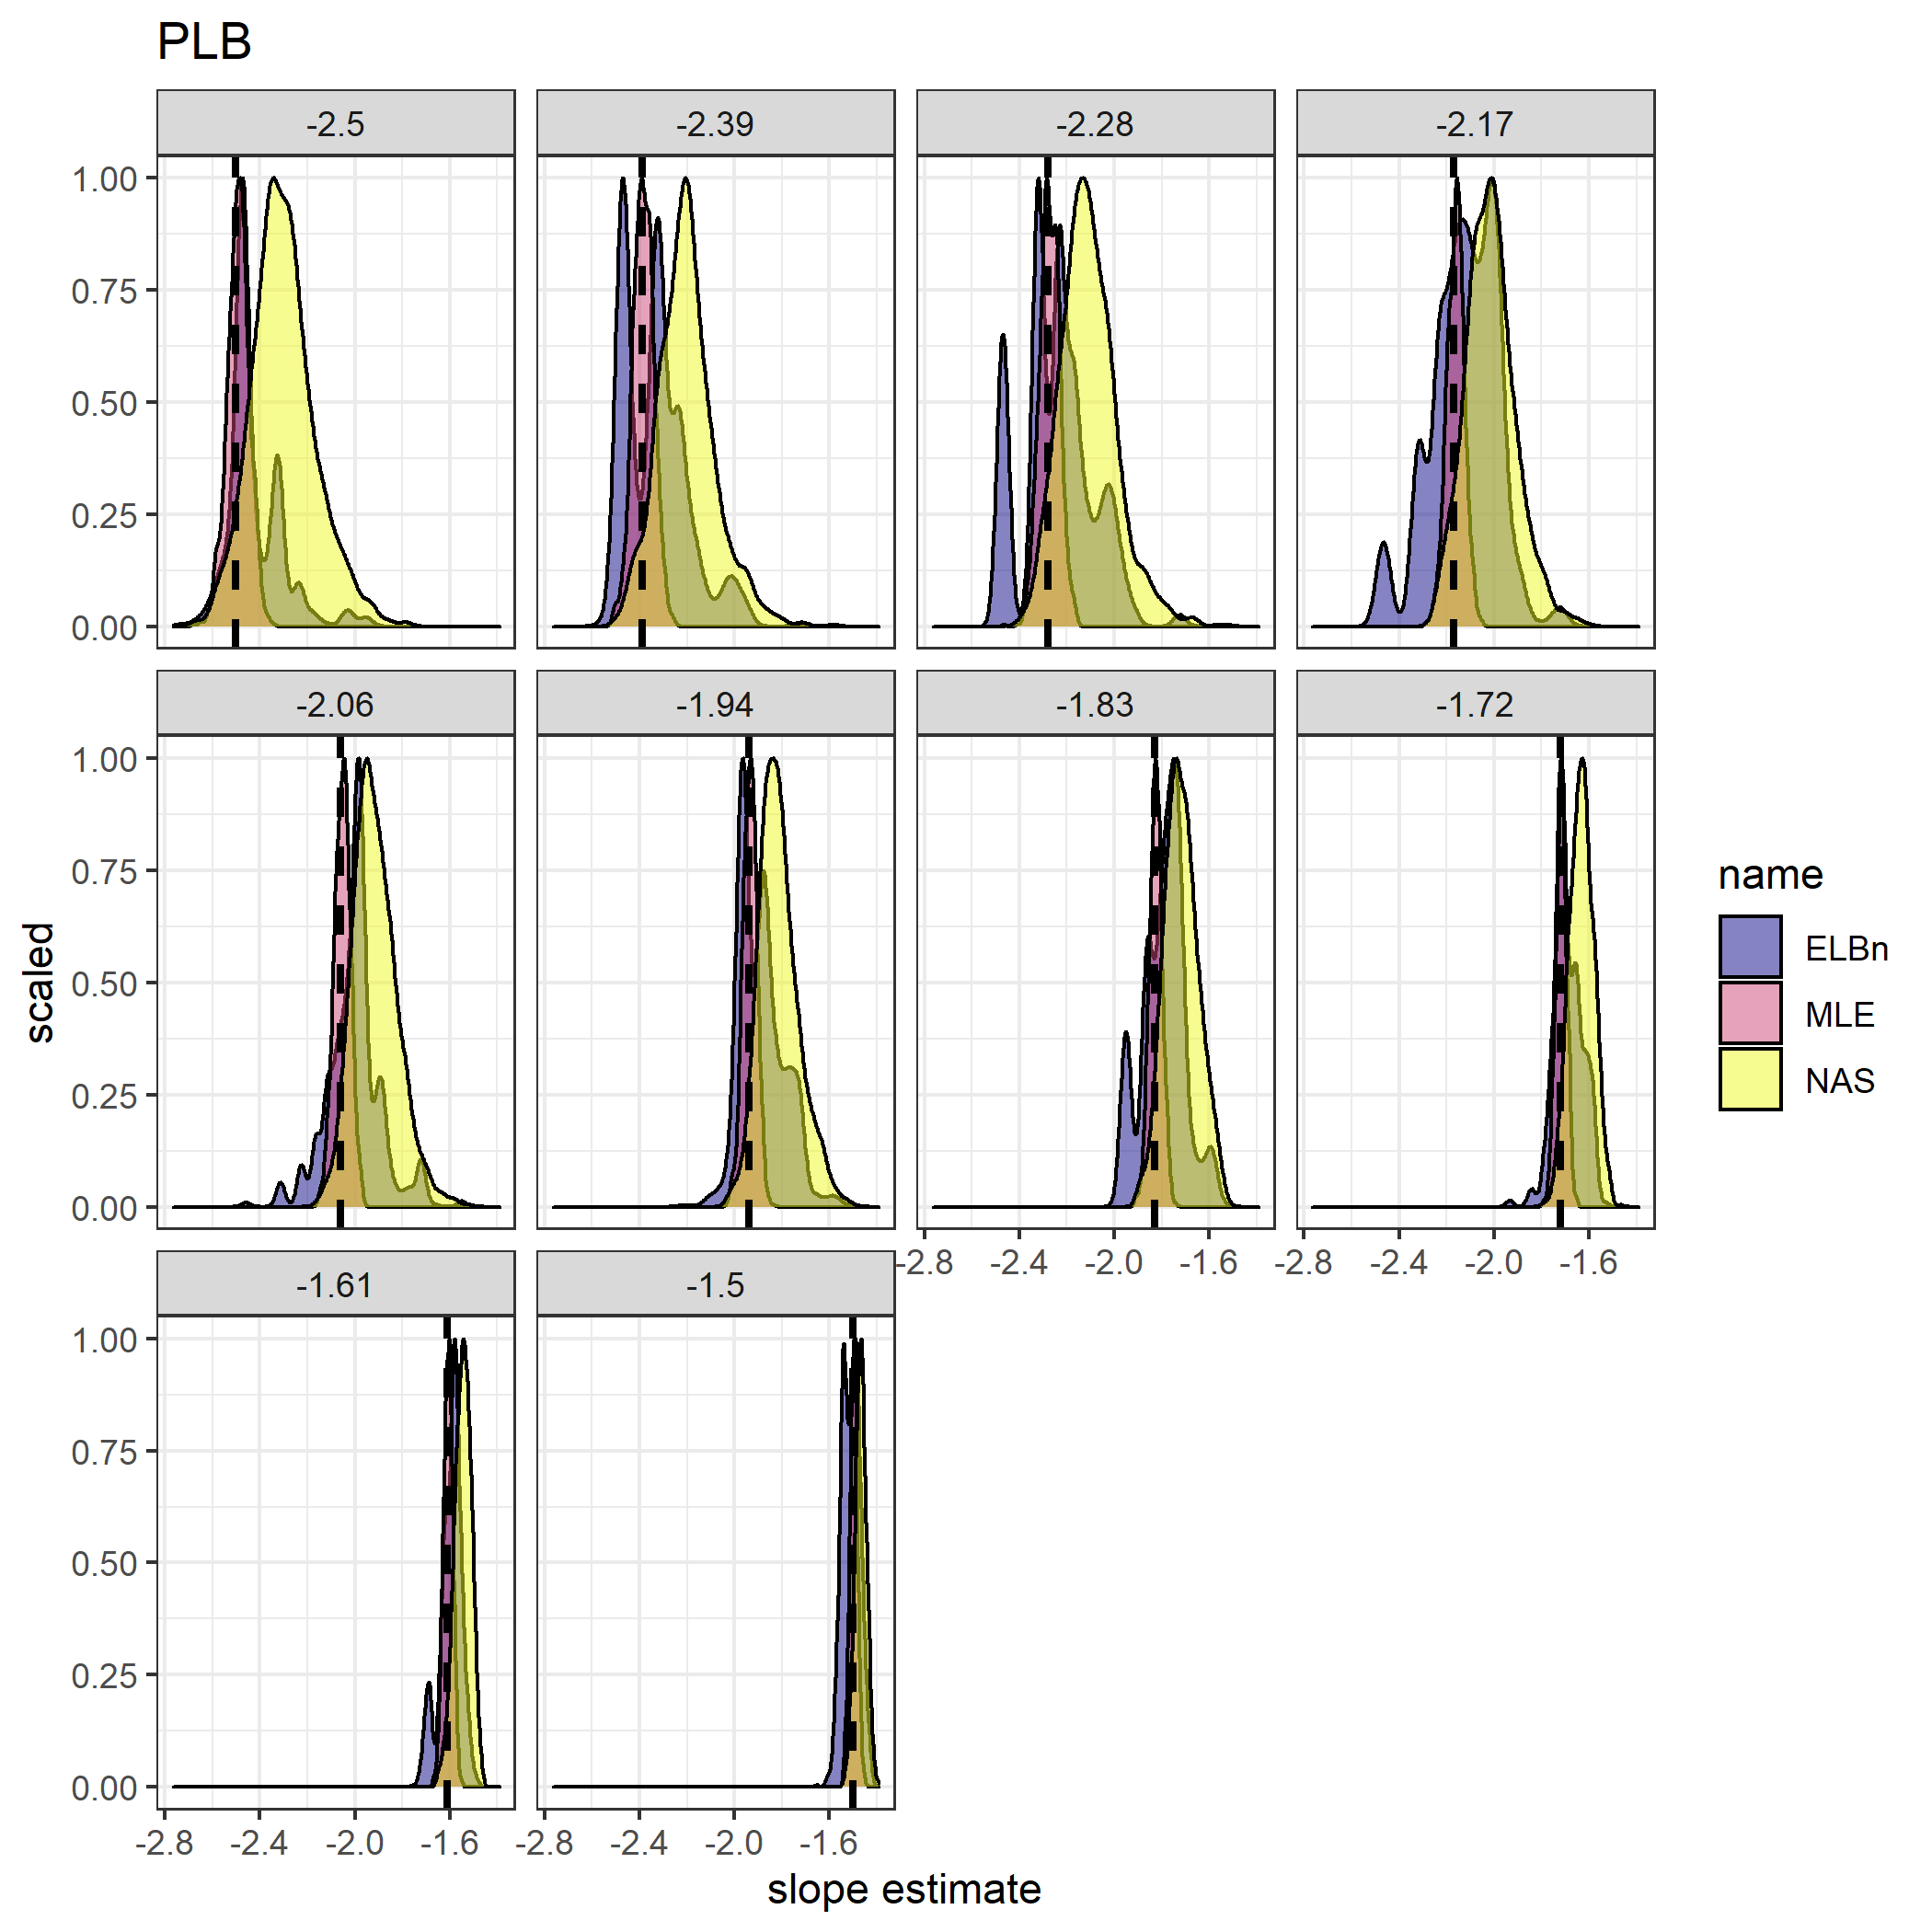
\includegraphics{figures/PLB_10_sites_est_b_density.png}
\caption{Distribution of estimated \(\lambda\) coefficient for ten sites
across a hypothetical gradient with known values. All other parameters
are the same as in the main analysis}
\end{figure}

\newpage

\begin{figure}
\centering
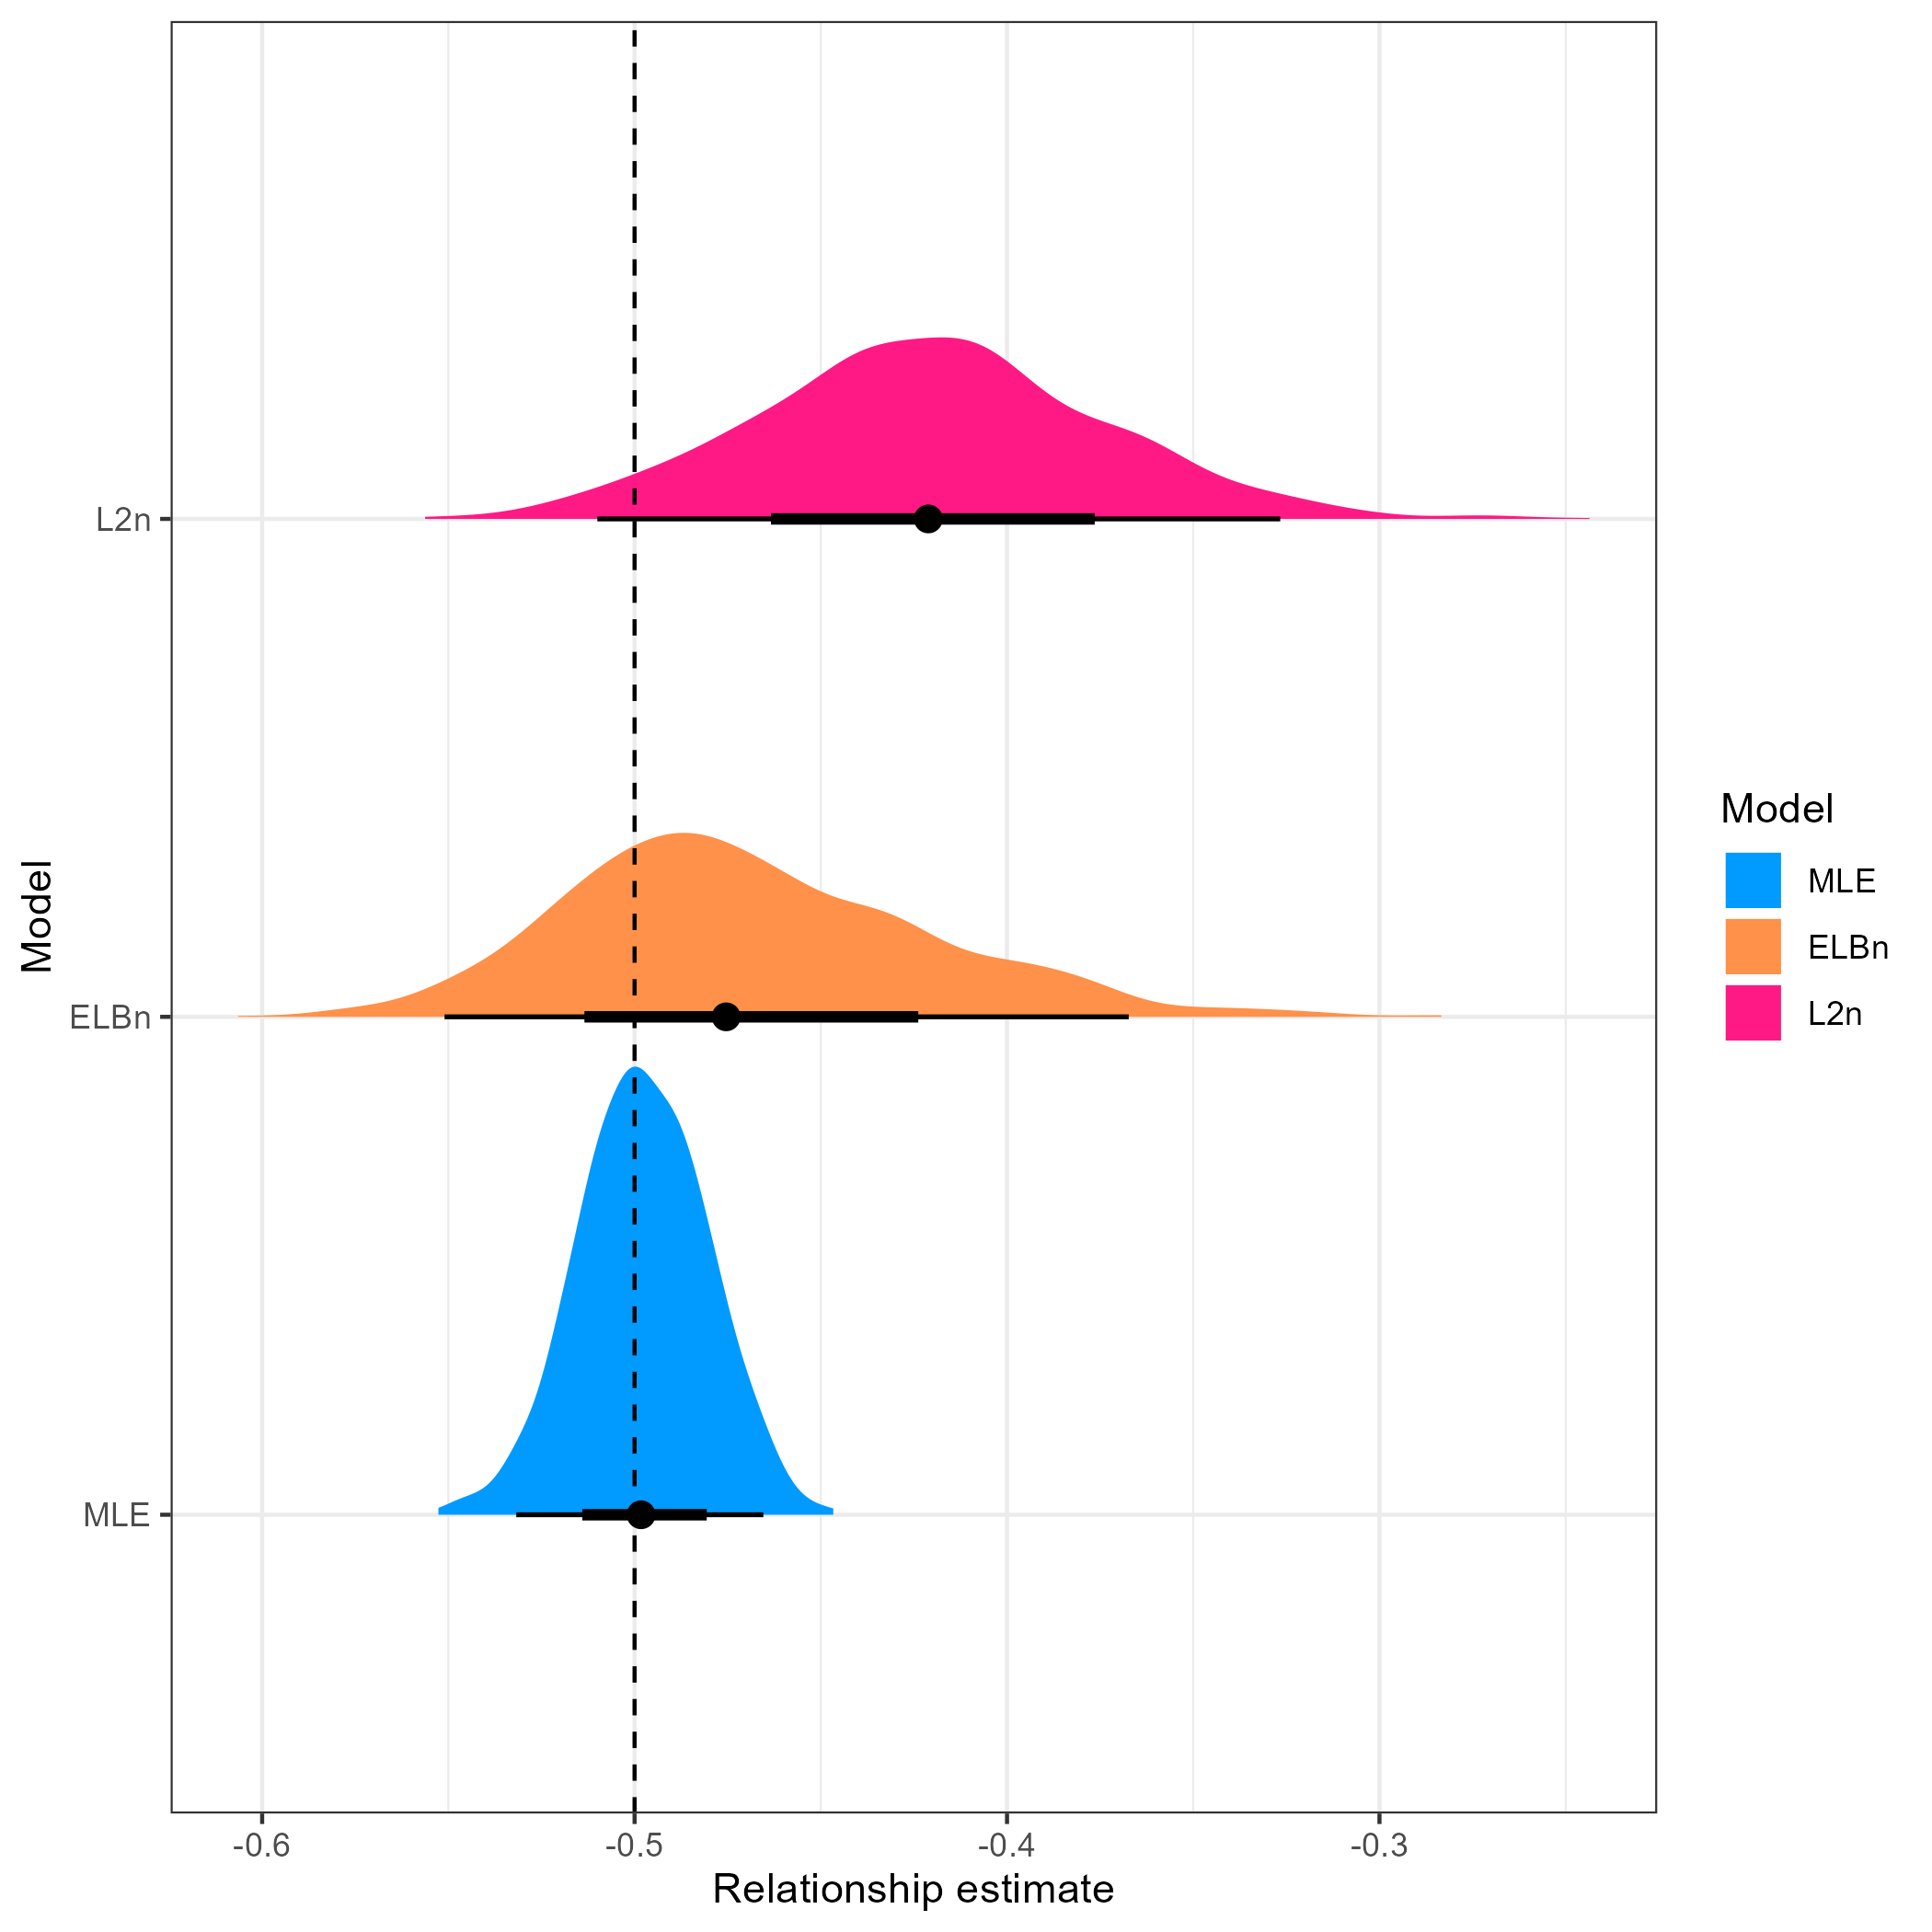
\includegraphics{figures/PLB_10_sites_relationship_density.png}
\caption{Distribution of estimated relationship (\(\beta_1\))
coefficient's for ten sites across a hypothetical gradient with known
value of 0.5. All other parameters are the same as in the main analysis}
\end{figure}

\newpage

\hypertarget{three-sites}{%
\subsubsection{Three sites}\label{three-sites}}

\begin{figure}
\centering
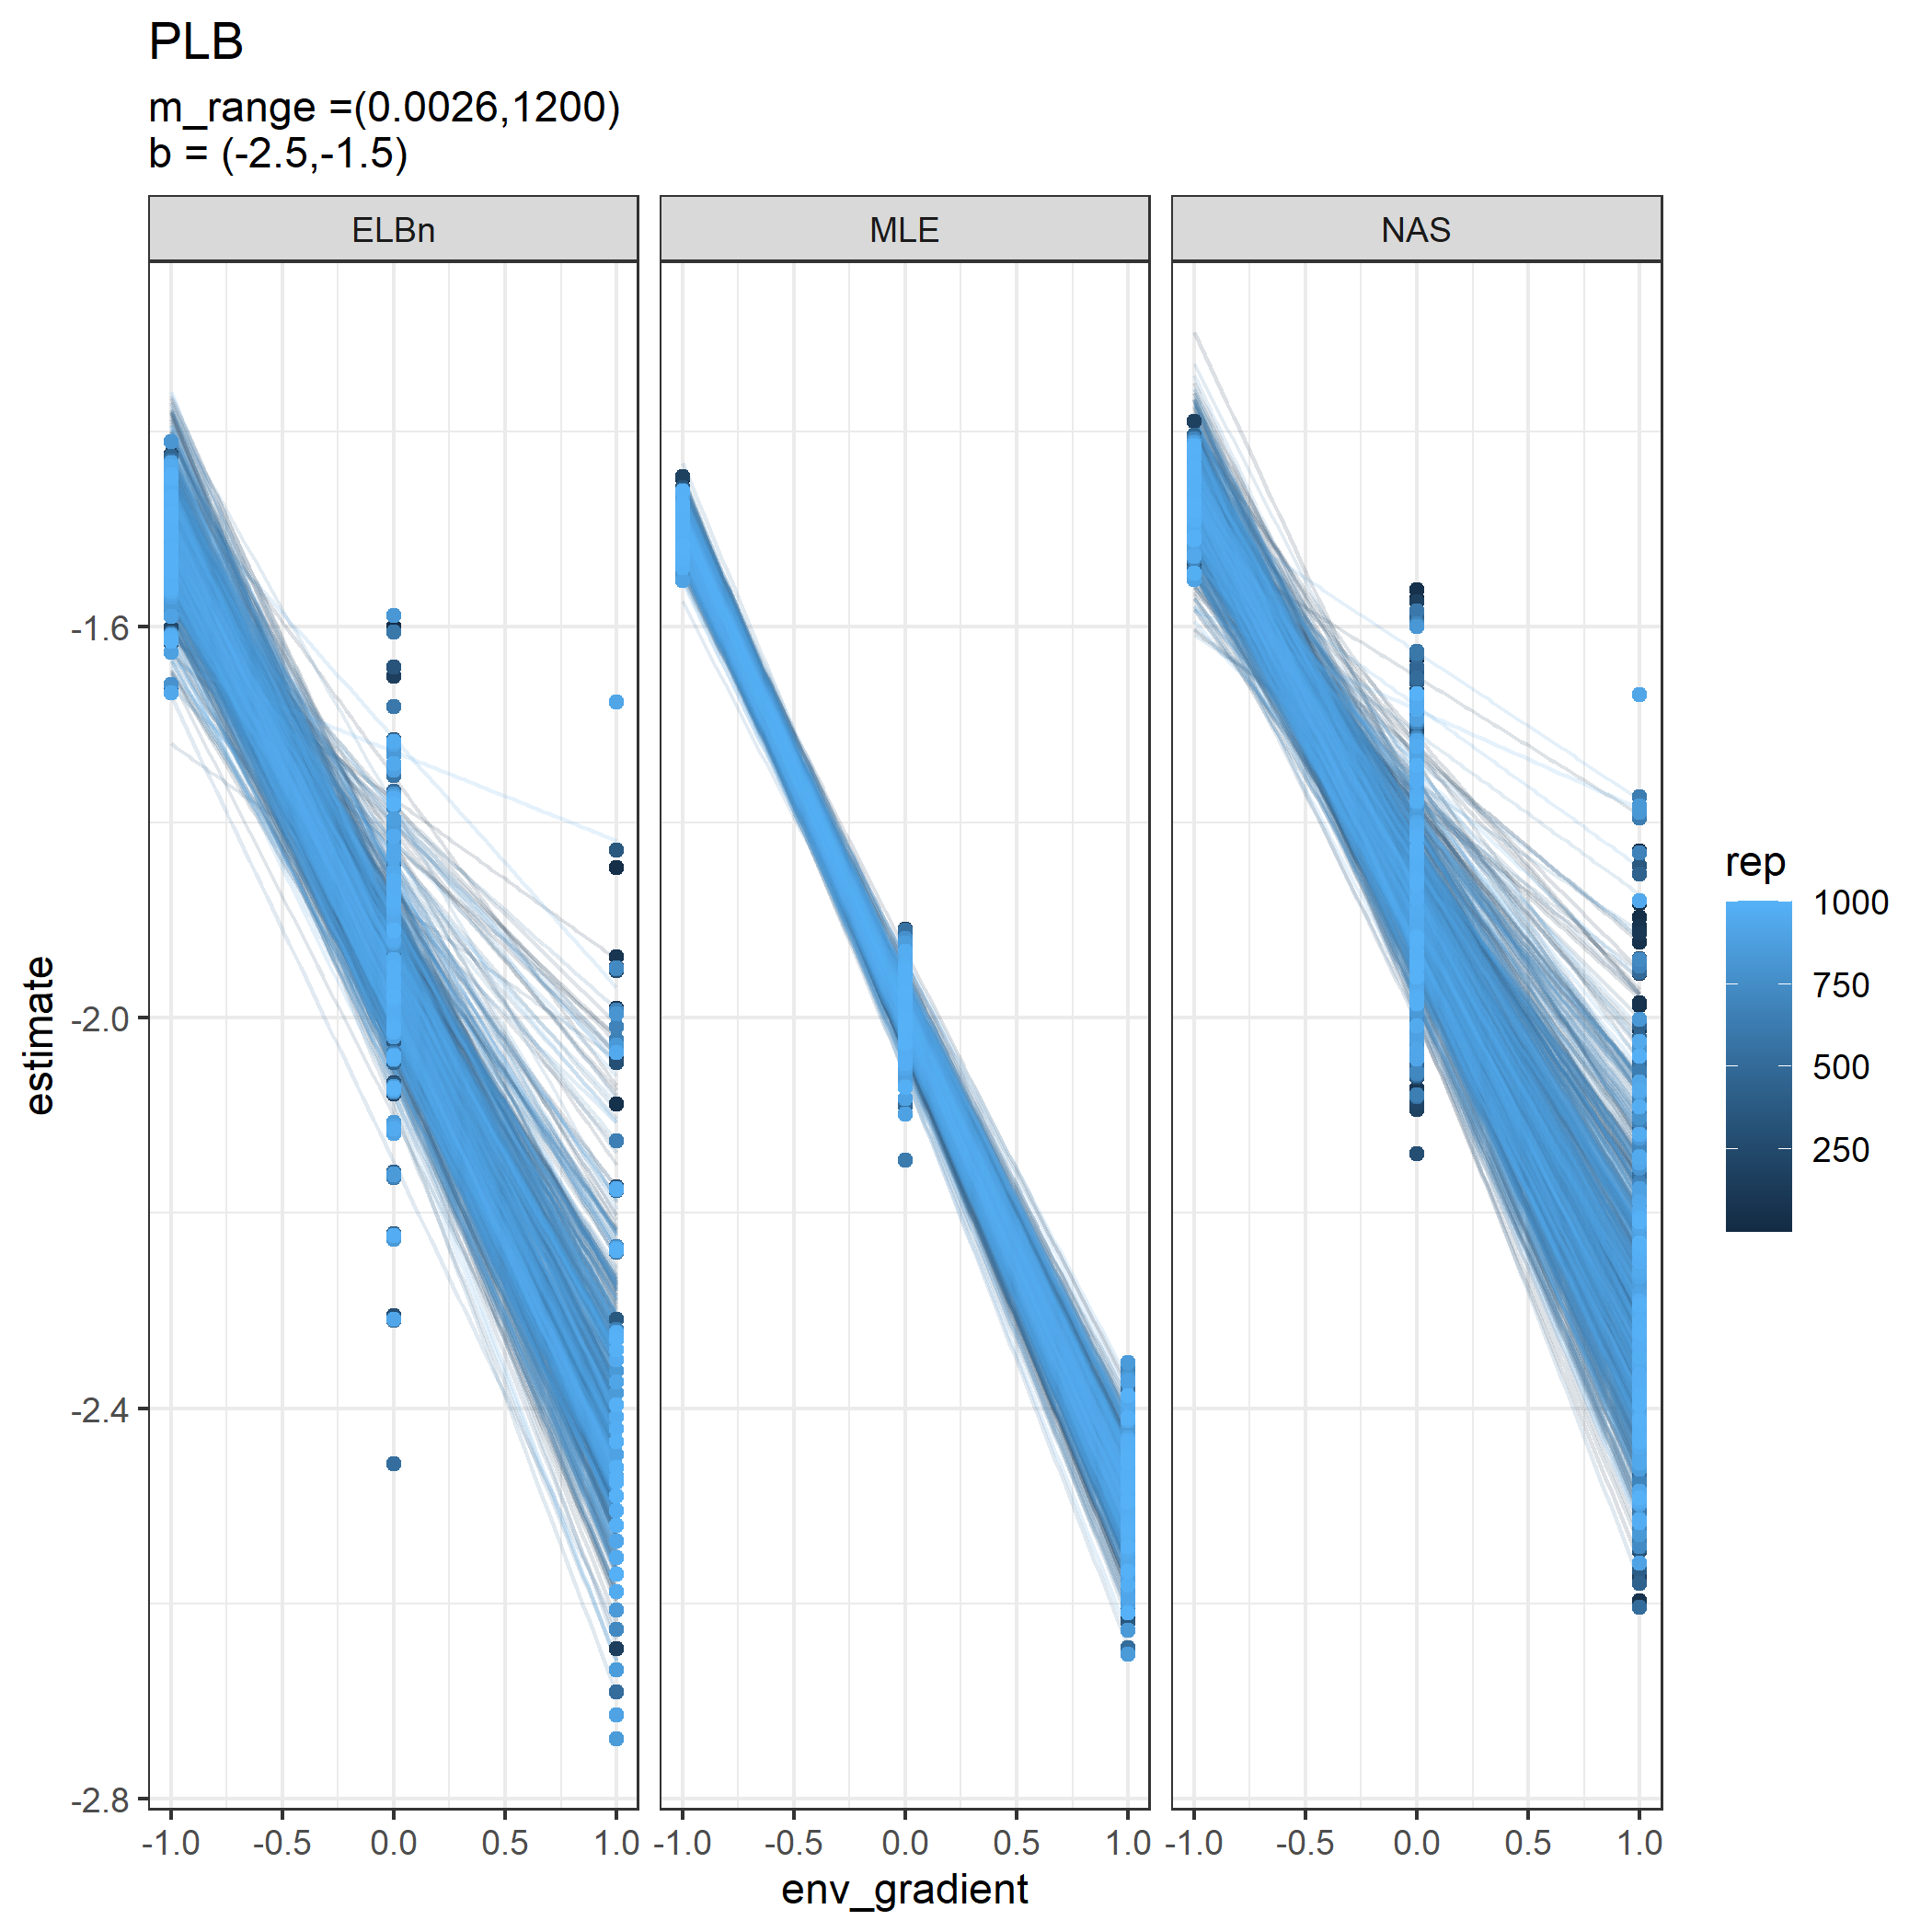
\includegraphics{figures/PLB_3_sites_main.png}
\caption{Individual regressions for three sites across a hypothetical
gradient with a known relationship of 0.5. All other parameters are the
same as in the main analysis.}
\end{figure}

\newpage

\begin{figure}
\centering
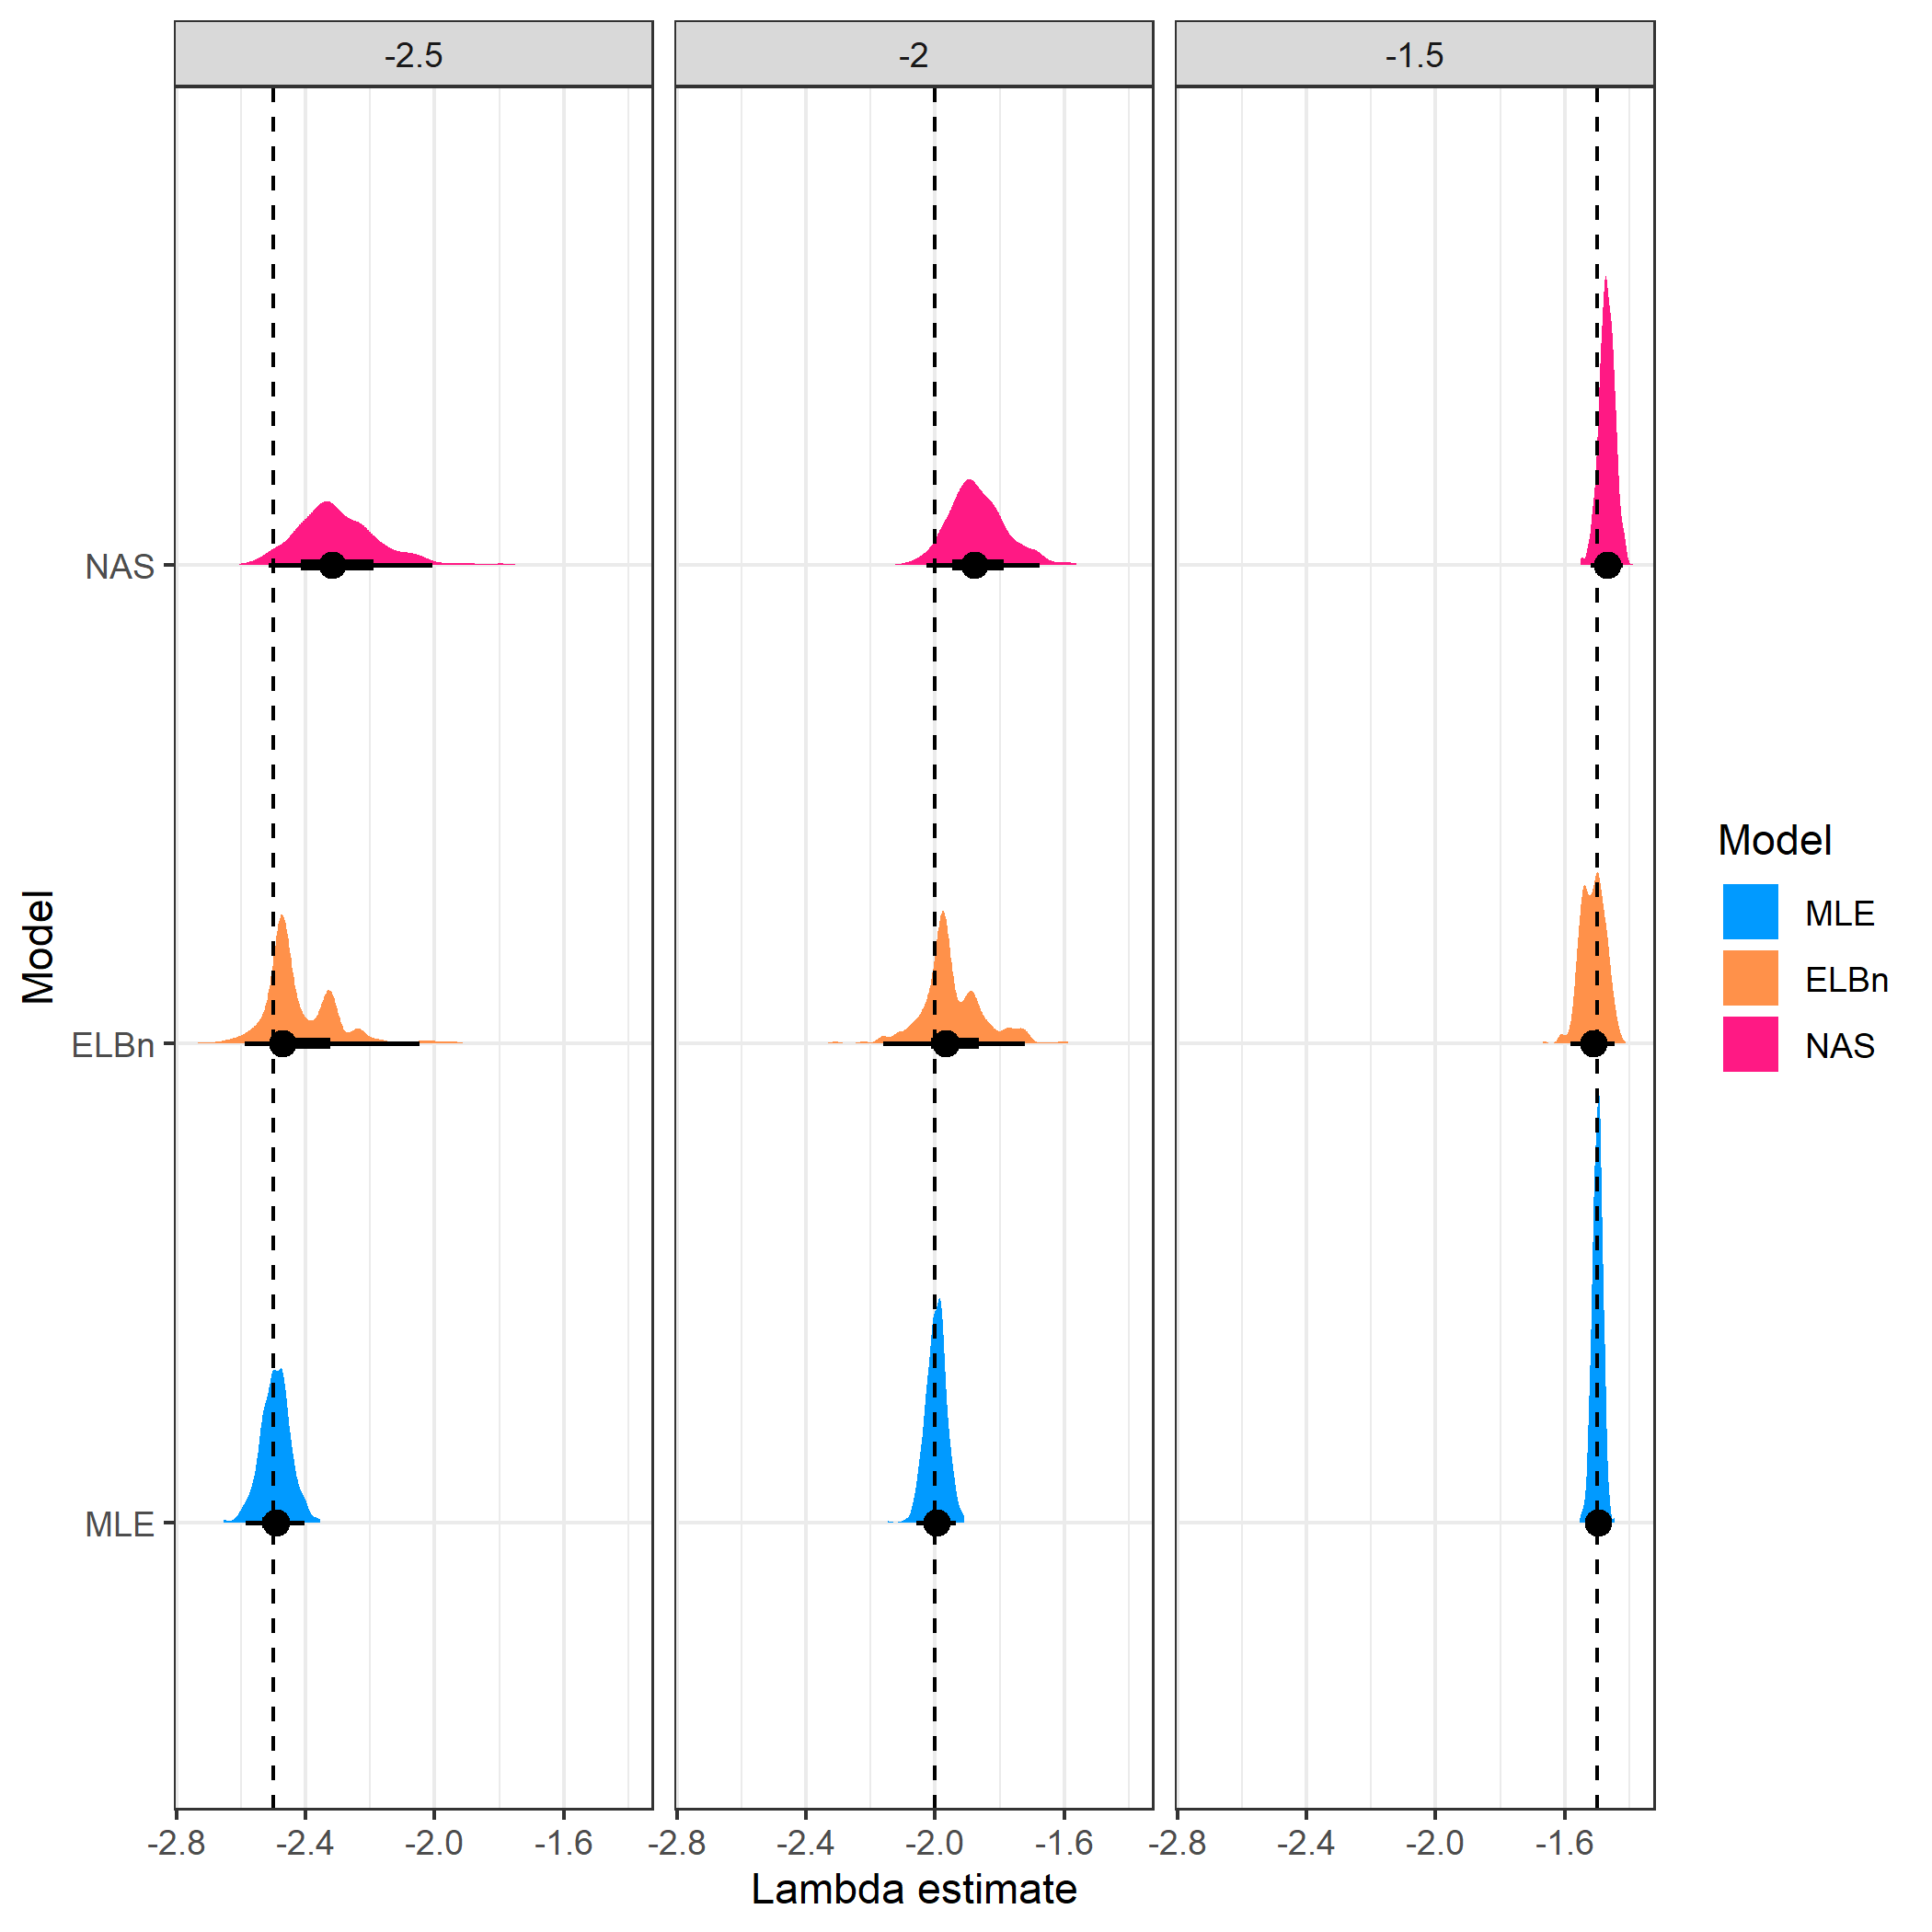
\includegraphics{figures/PLB_3_sites_est_b_density.png}
\caption{Distribution of estimated \(\lambda\) coefficient for three
sites across a hypothetical gradient with known values. All other
parameters are the same as in the main analysis.}
\end{figure}

\newpage

\begin{figure}
\centering
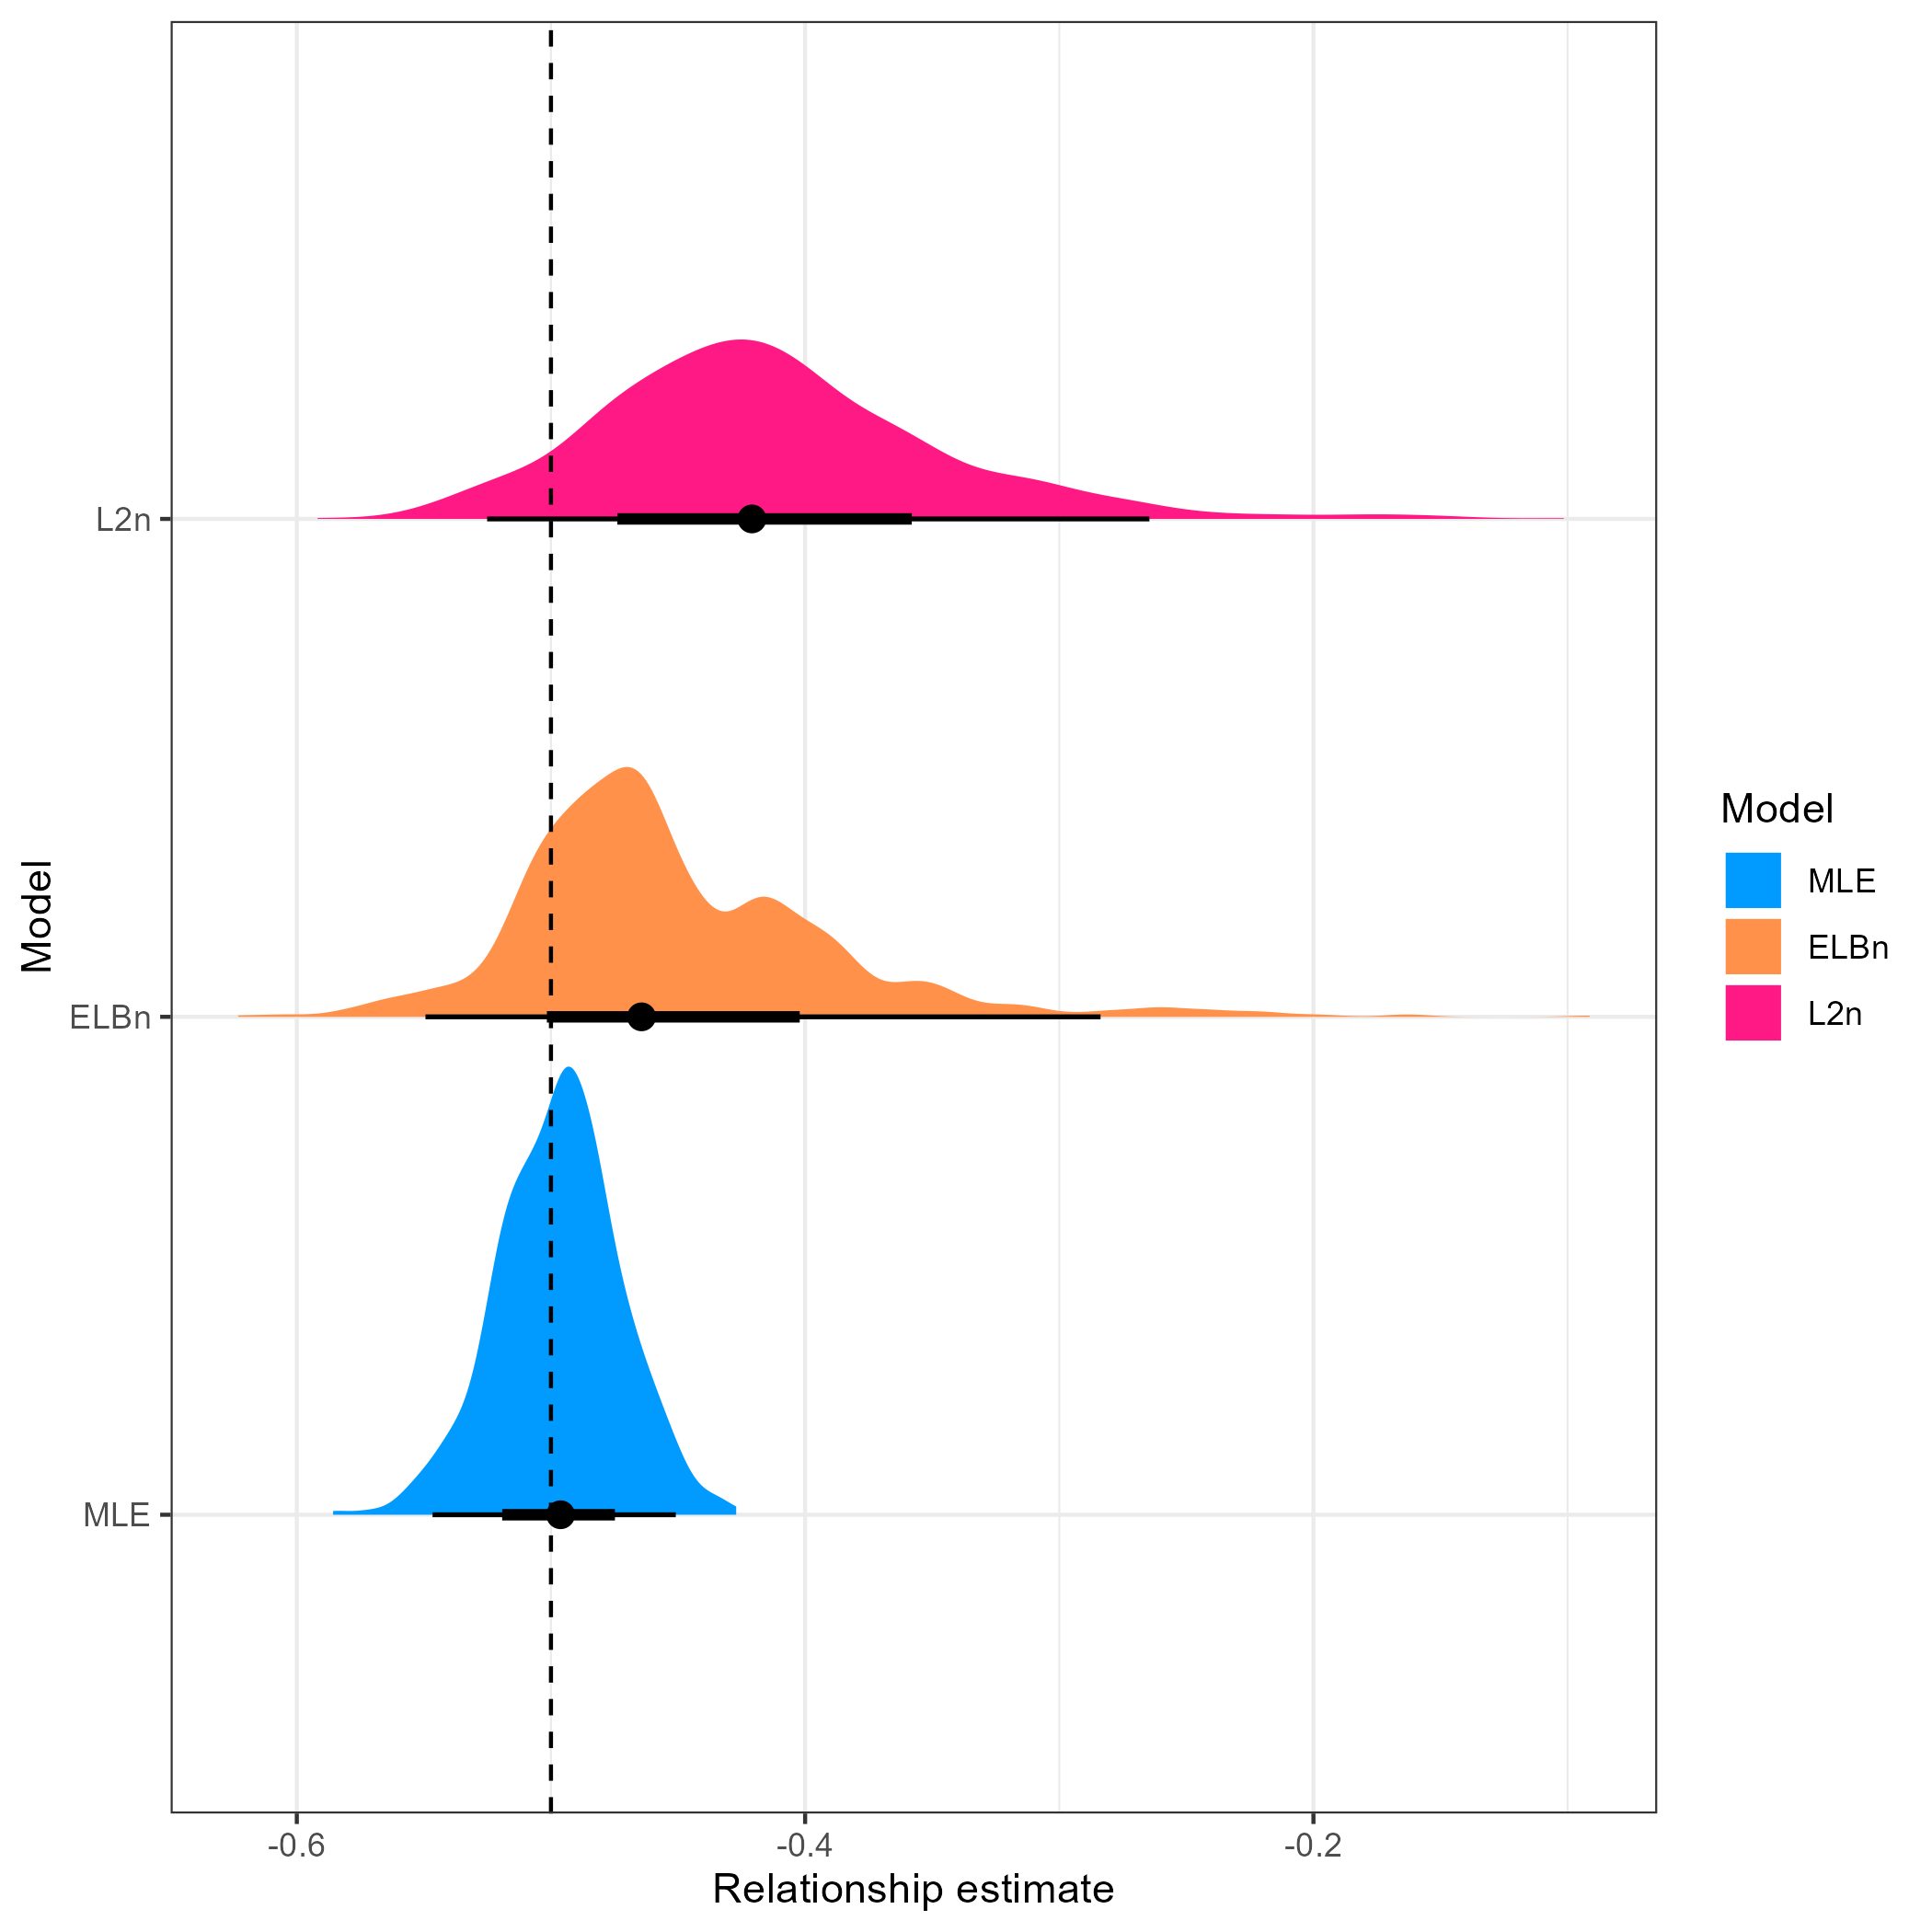
\includegraphics{figures/PLB_3_sites_relationship_density.png}
\caption{Distribution of estimated relationship (\(\beta_1\))
coefficient's for three sites across a hypothetical gradient with known
value of 0.5. All other parameters are the same as in the main analysis}
\end{figure}

\newpage

\hypertarget{large-environmental-gradient}{%
\subsection{Large environmental
gradient}\label{large-environmental-gradient}}

\begin{figure}
\centering
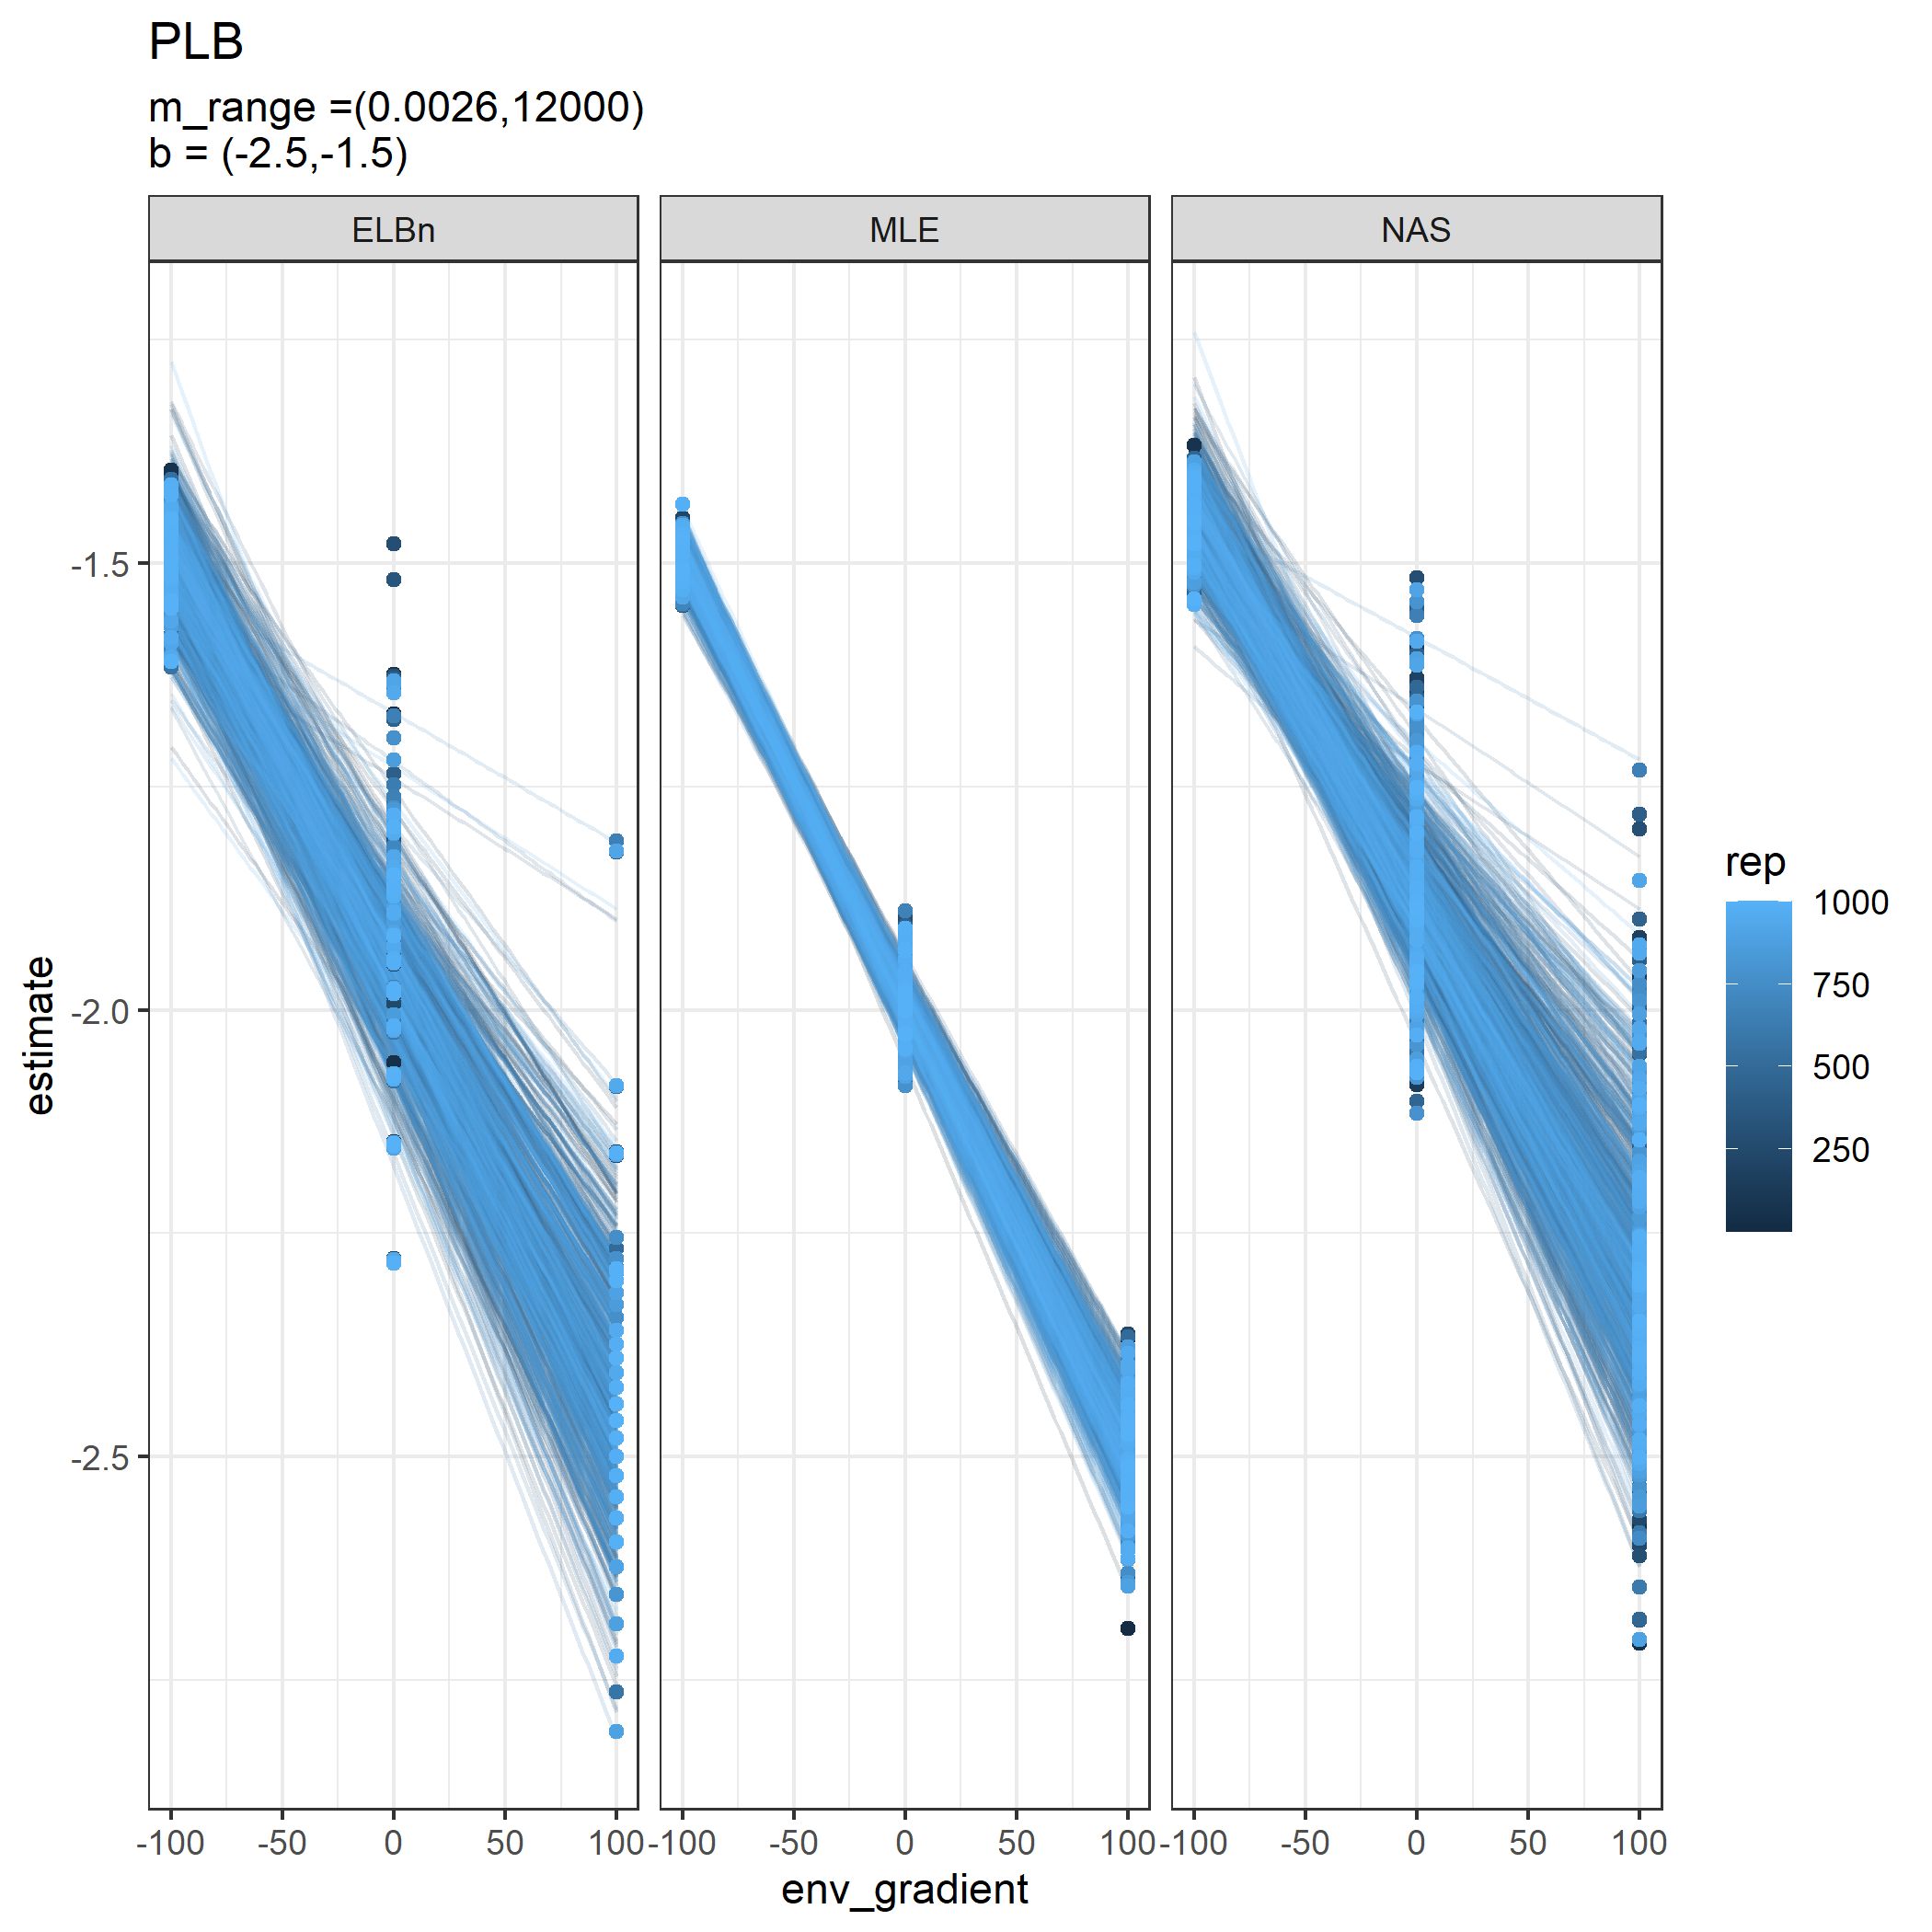
\includegraphics{figures/PLB_large_x_main.png}
\caption{Individual regressions for five sites across a hypothetical
gradient with a known relationship of 0.5. Range of environmental values
(\emph{x}-axis) increased to be -1000, to 1000.}
\end{figure}

\newpage

\begin{figure}
\centering
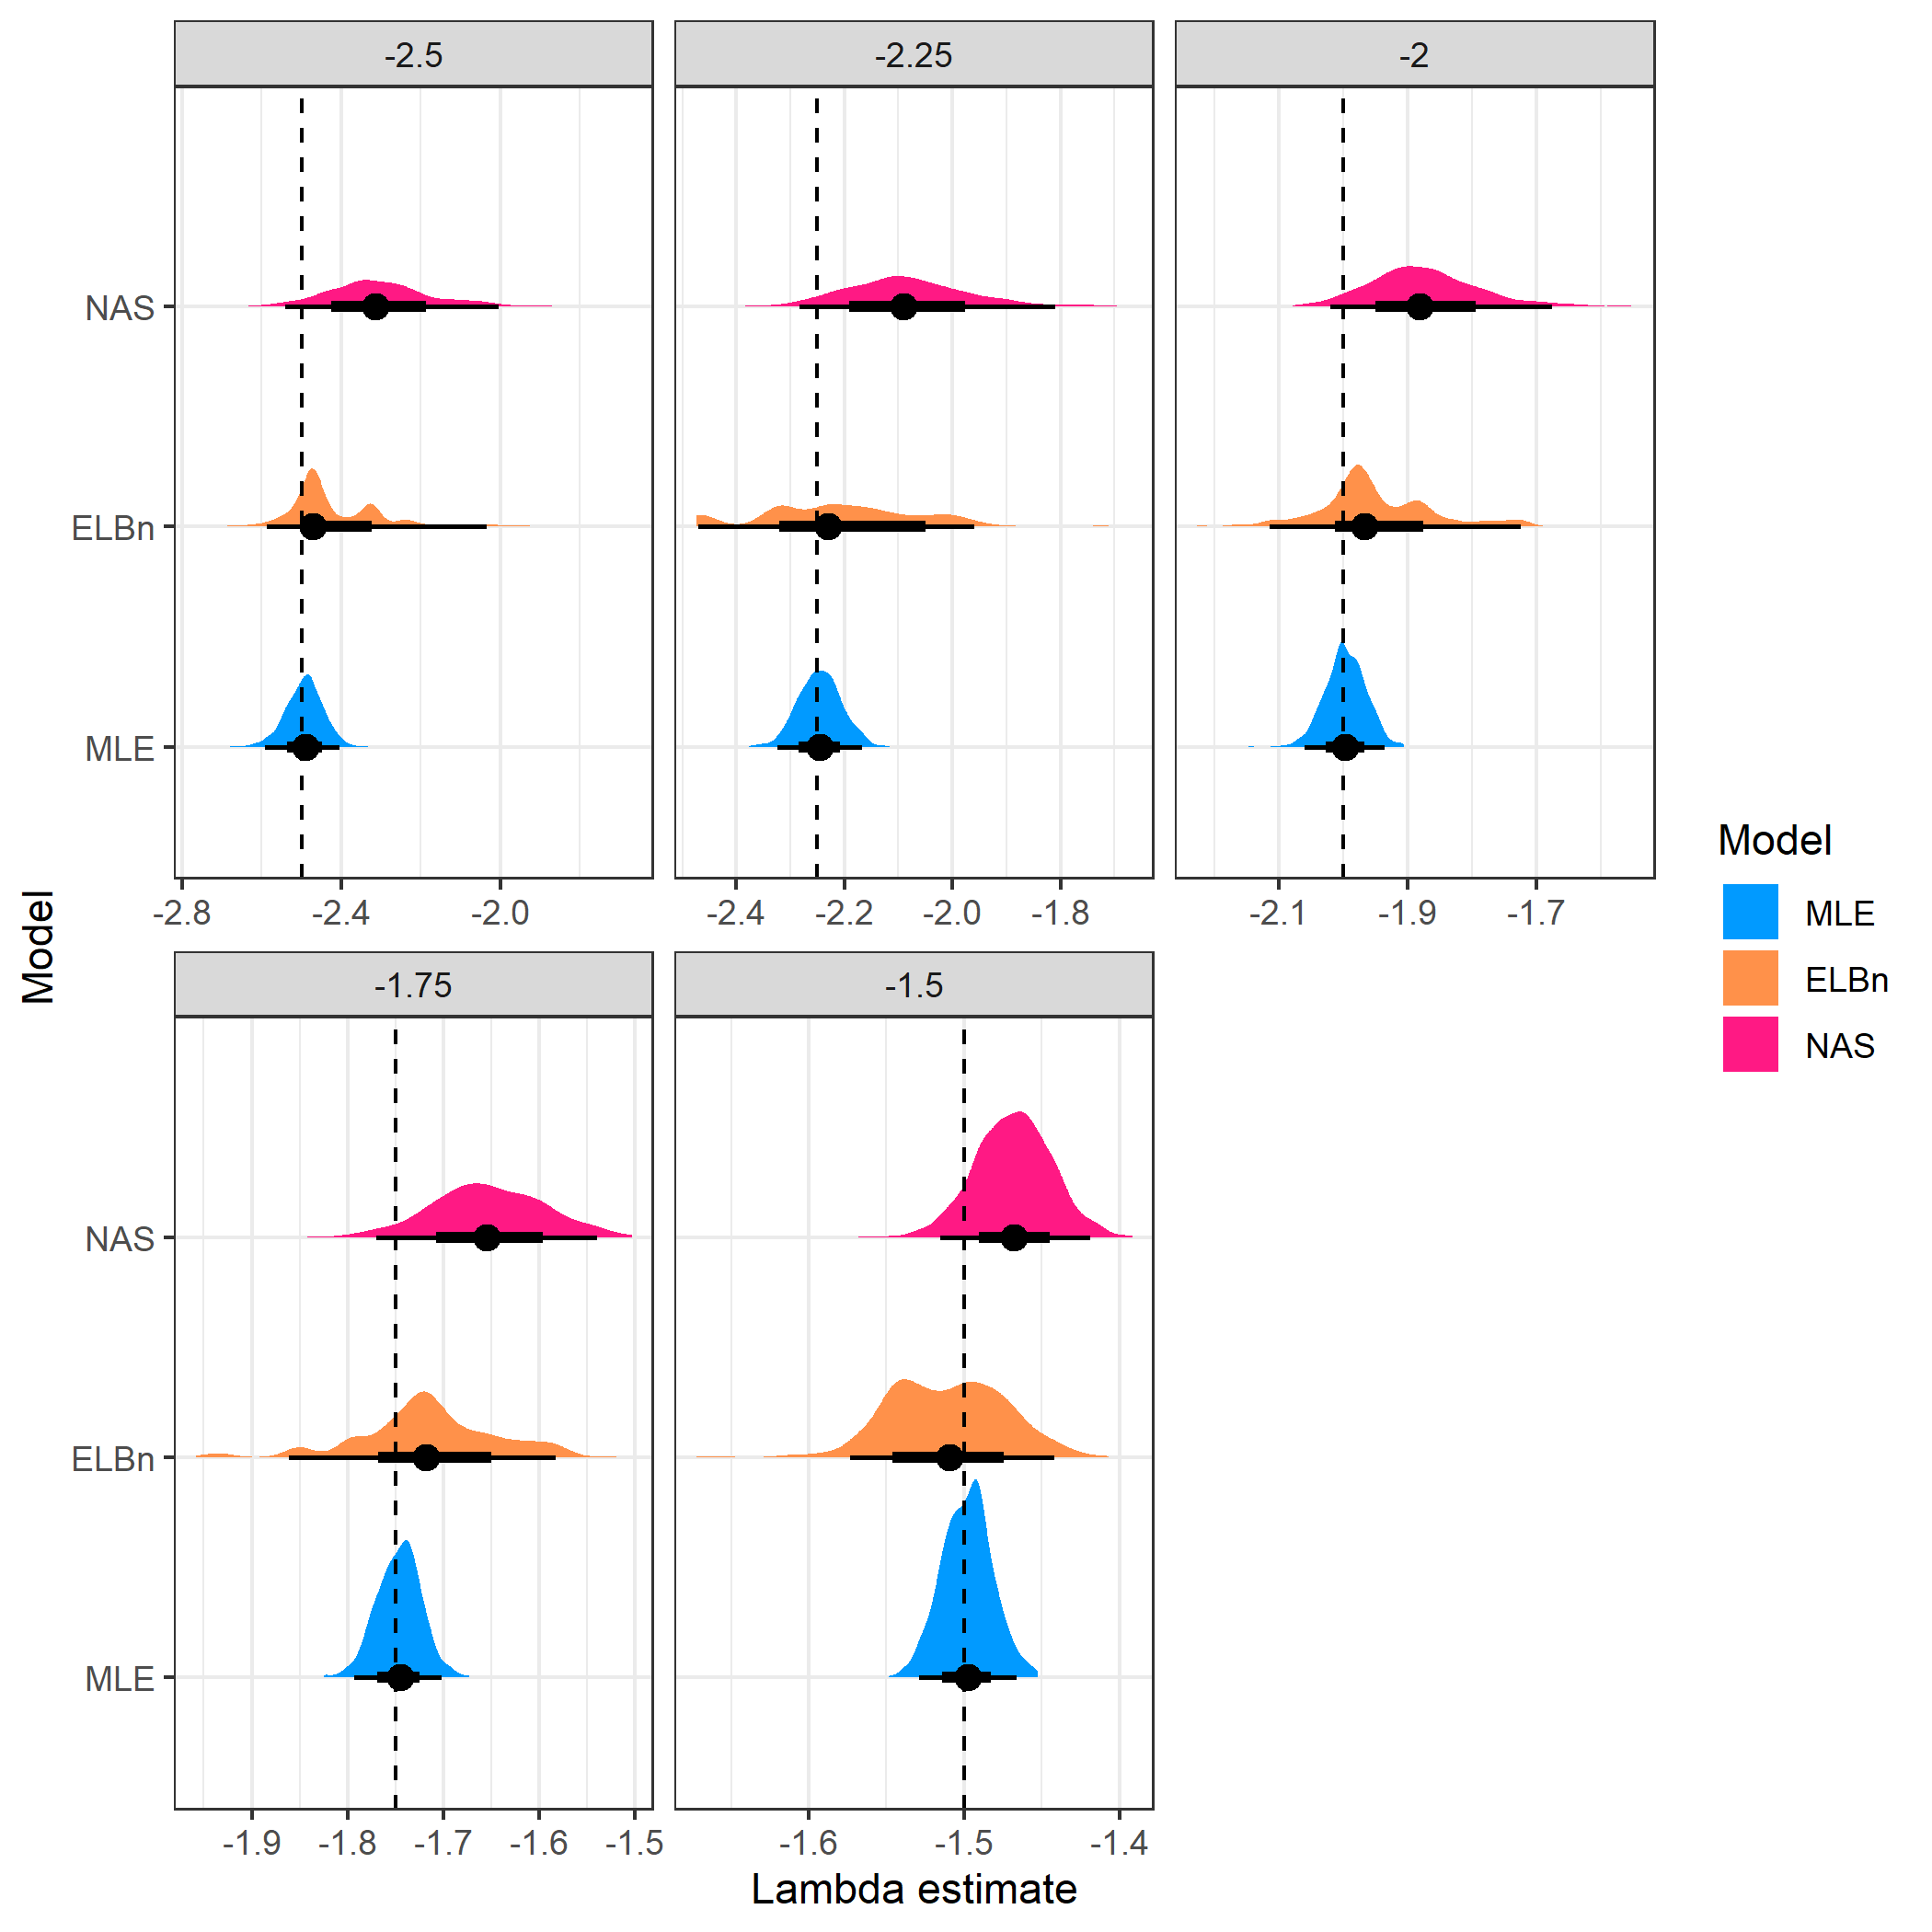
\includegraphics{figures/PLB_large_x_est_b_density.png}
\caption{Distribution of estimated \(\lambda\) coefficient for five
sites across a hypothetical gradient with known values. Range of
environmental values (\emph{x}-axis) increased to be -1000, to 1000.}
\end{figure}

\newpage

\begin{figure}
\centering
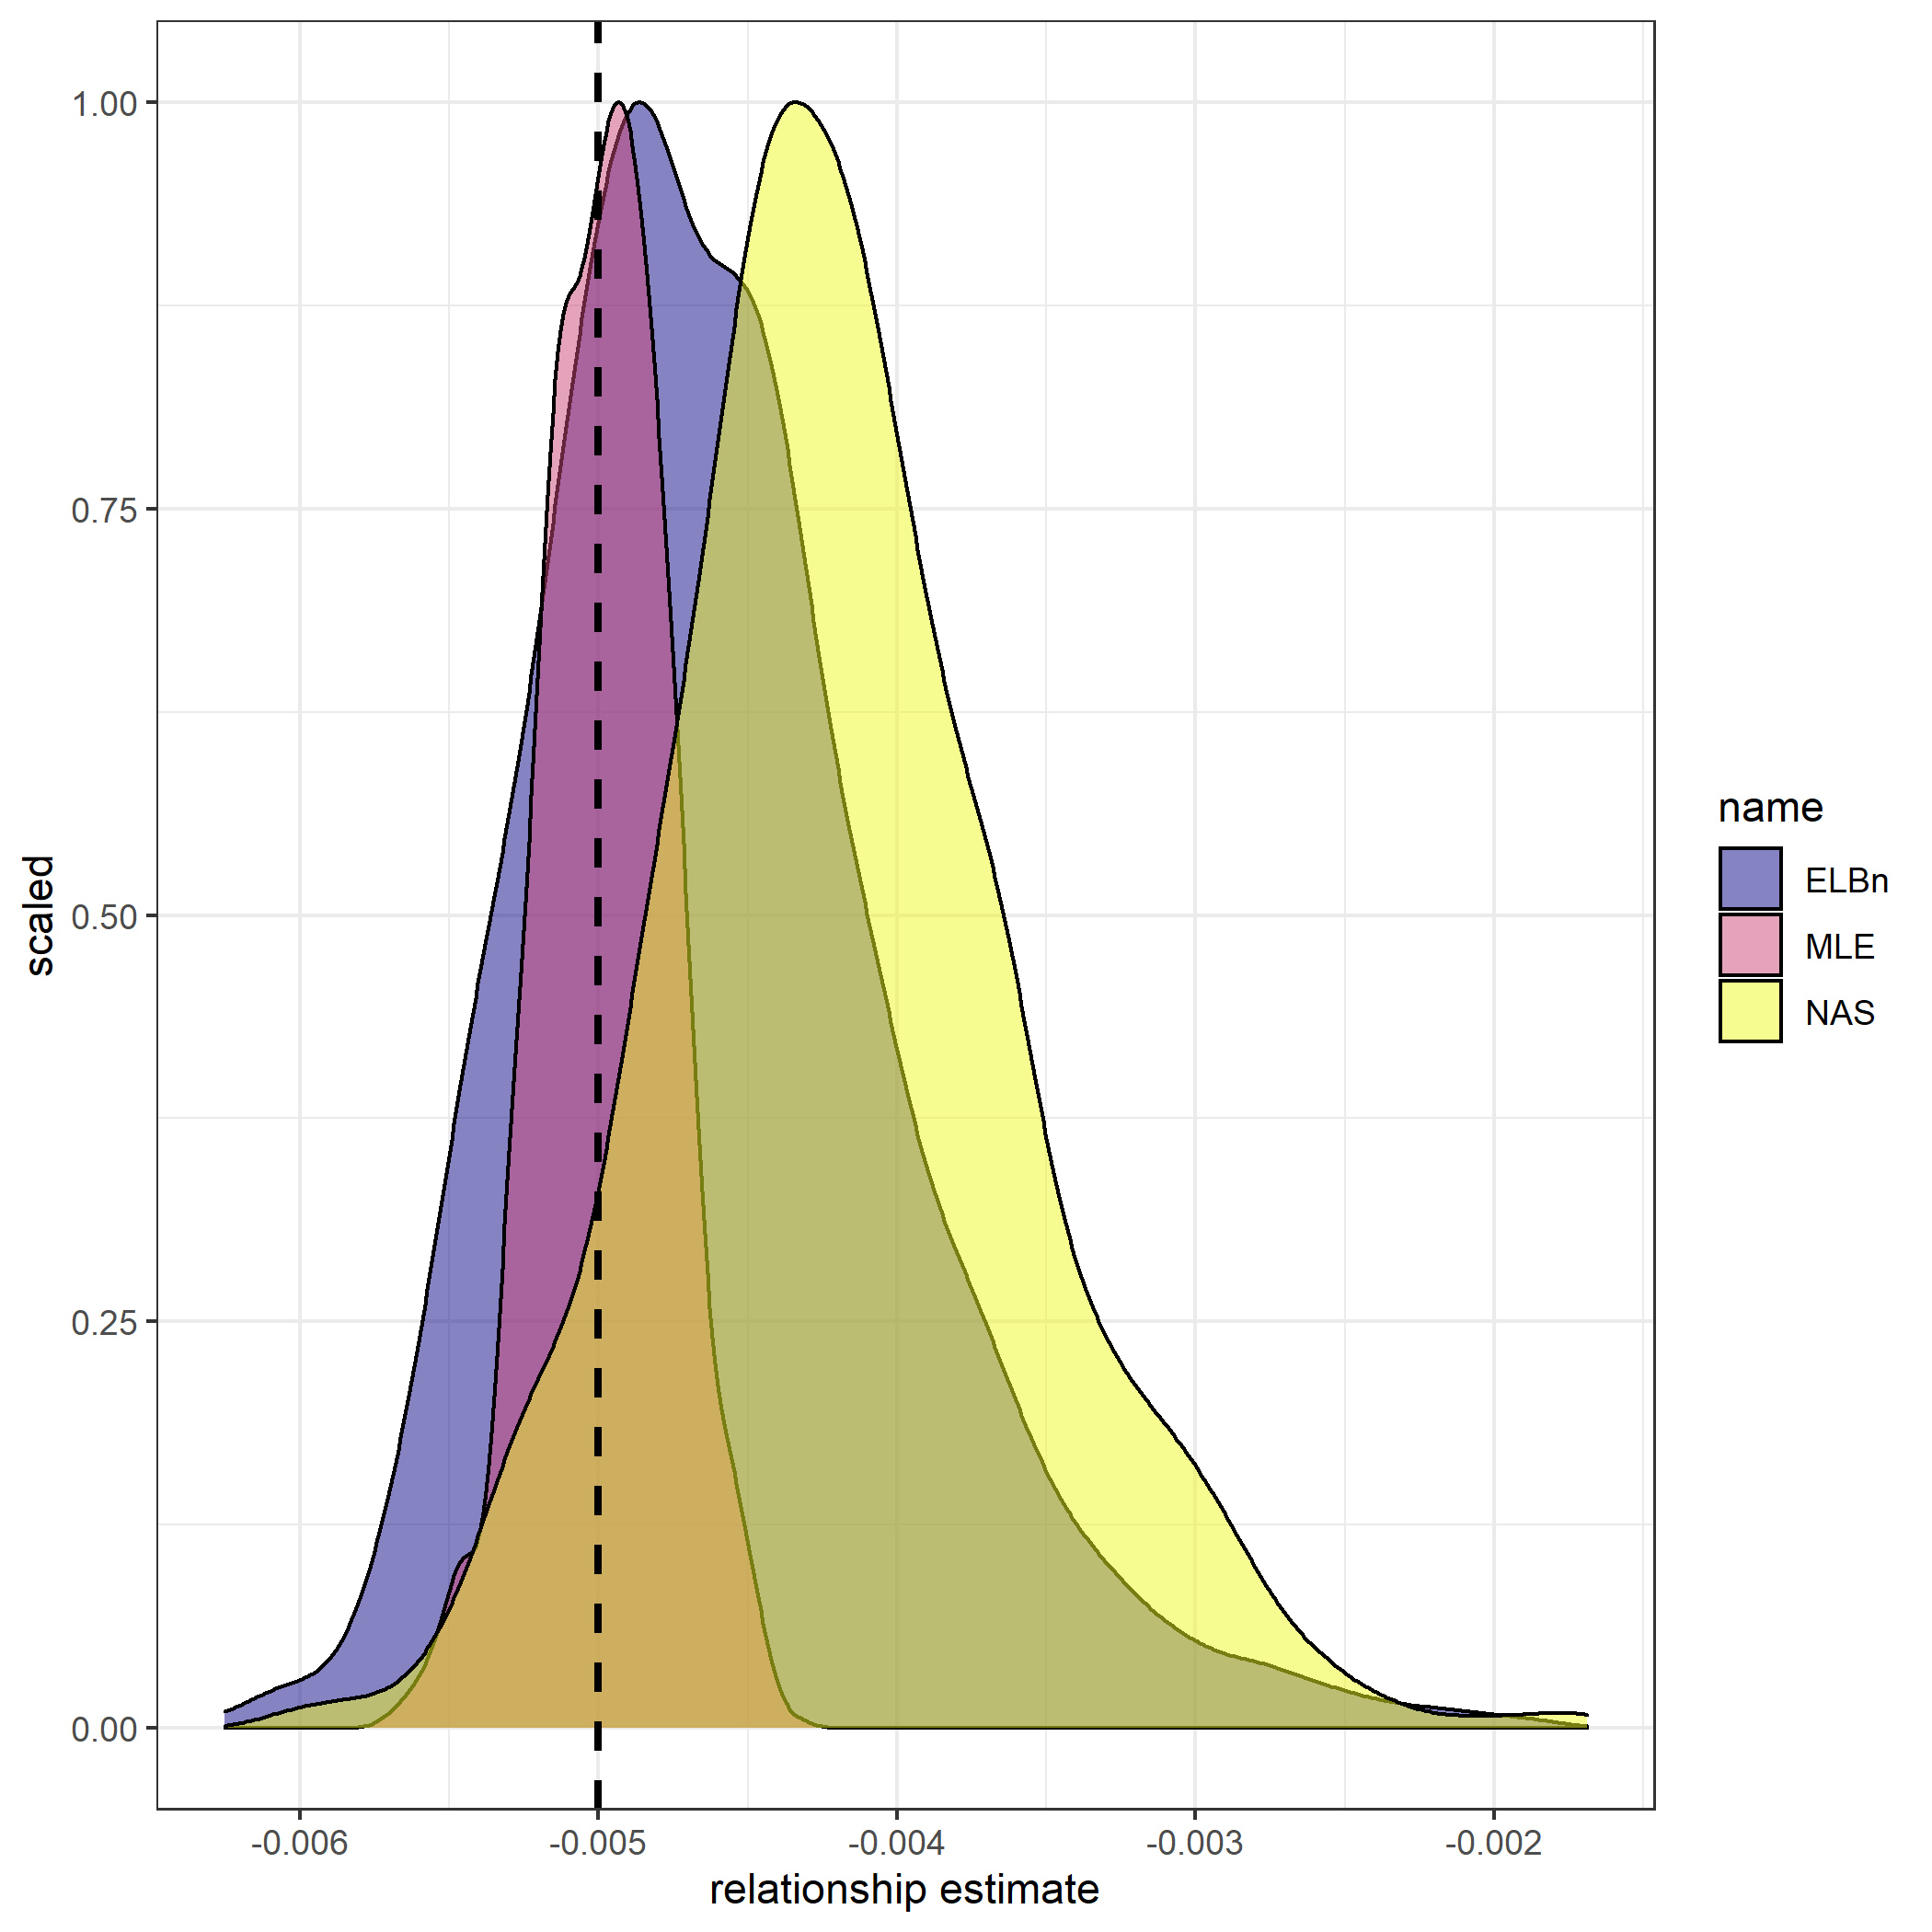
\includegraphics{figures/PLB_large_x_relationship_density.png}
\caption{Distribution of estimated relationship (\(\beta_1\))
coefficient's for five sites across a hypothetical gradient with known
value of 0.5. Range of environmental values (\emph{x}-axis) increased to
be -1000, to 1000.}
\end{figure}

\newpage

\hypertarget{range-of-body-sizes-m}{%
\subsection{\texorpdfstring{Range of body sizes,
\(M\)}{Range of body sizes, M}}\label{range-of-body-sizes-m}}

\begin{figure}
\centering
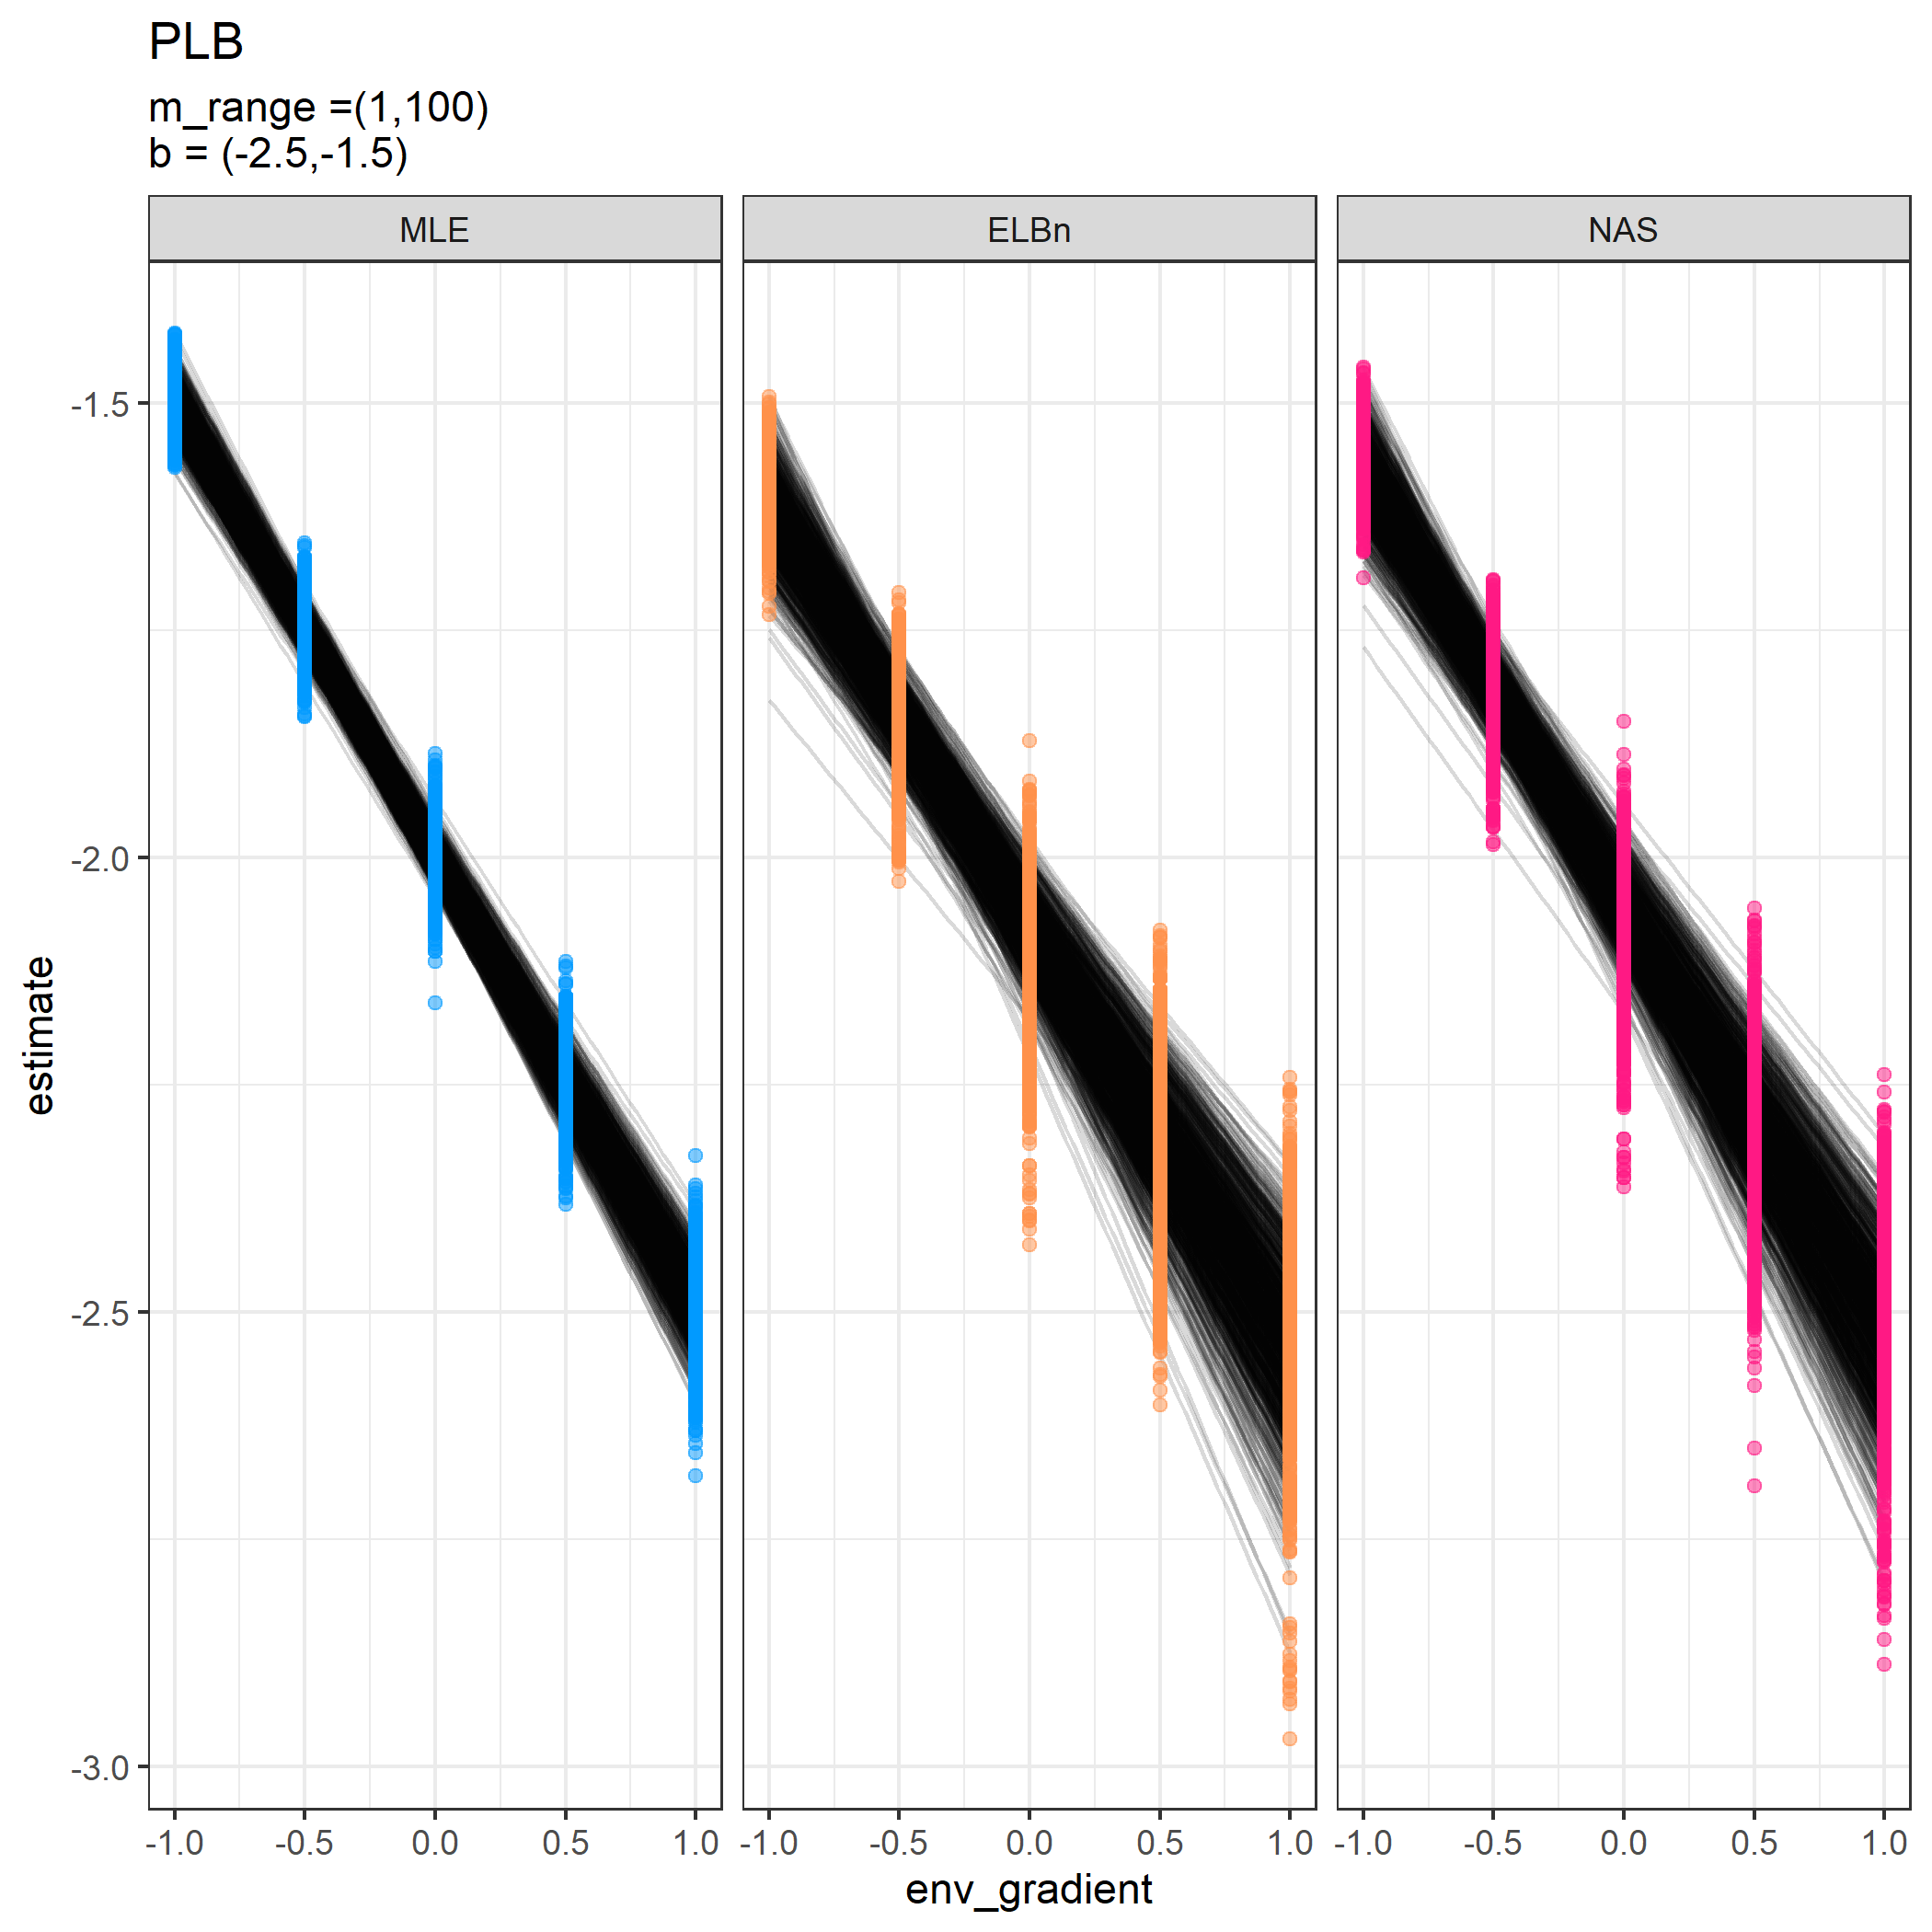
\includegraphics{figures/PLB_small_m_main.png}
\caption{Individual regressions for five sites across a hypothetical
gradient with a known relationship of 0.5. Range of body sizes is
reduced and is from 1, to 100.}
\end{figure}

\newpage

\begin{figure}
\centering
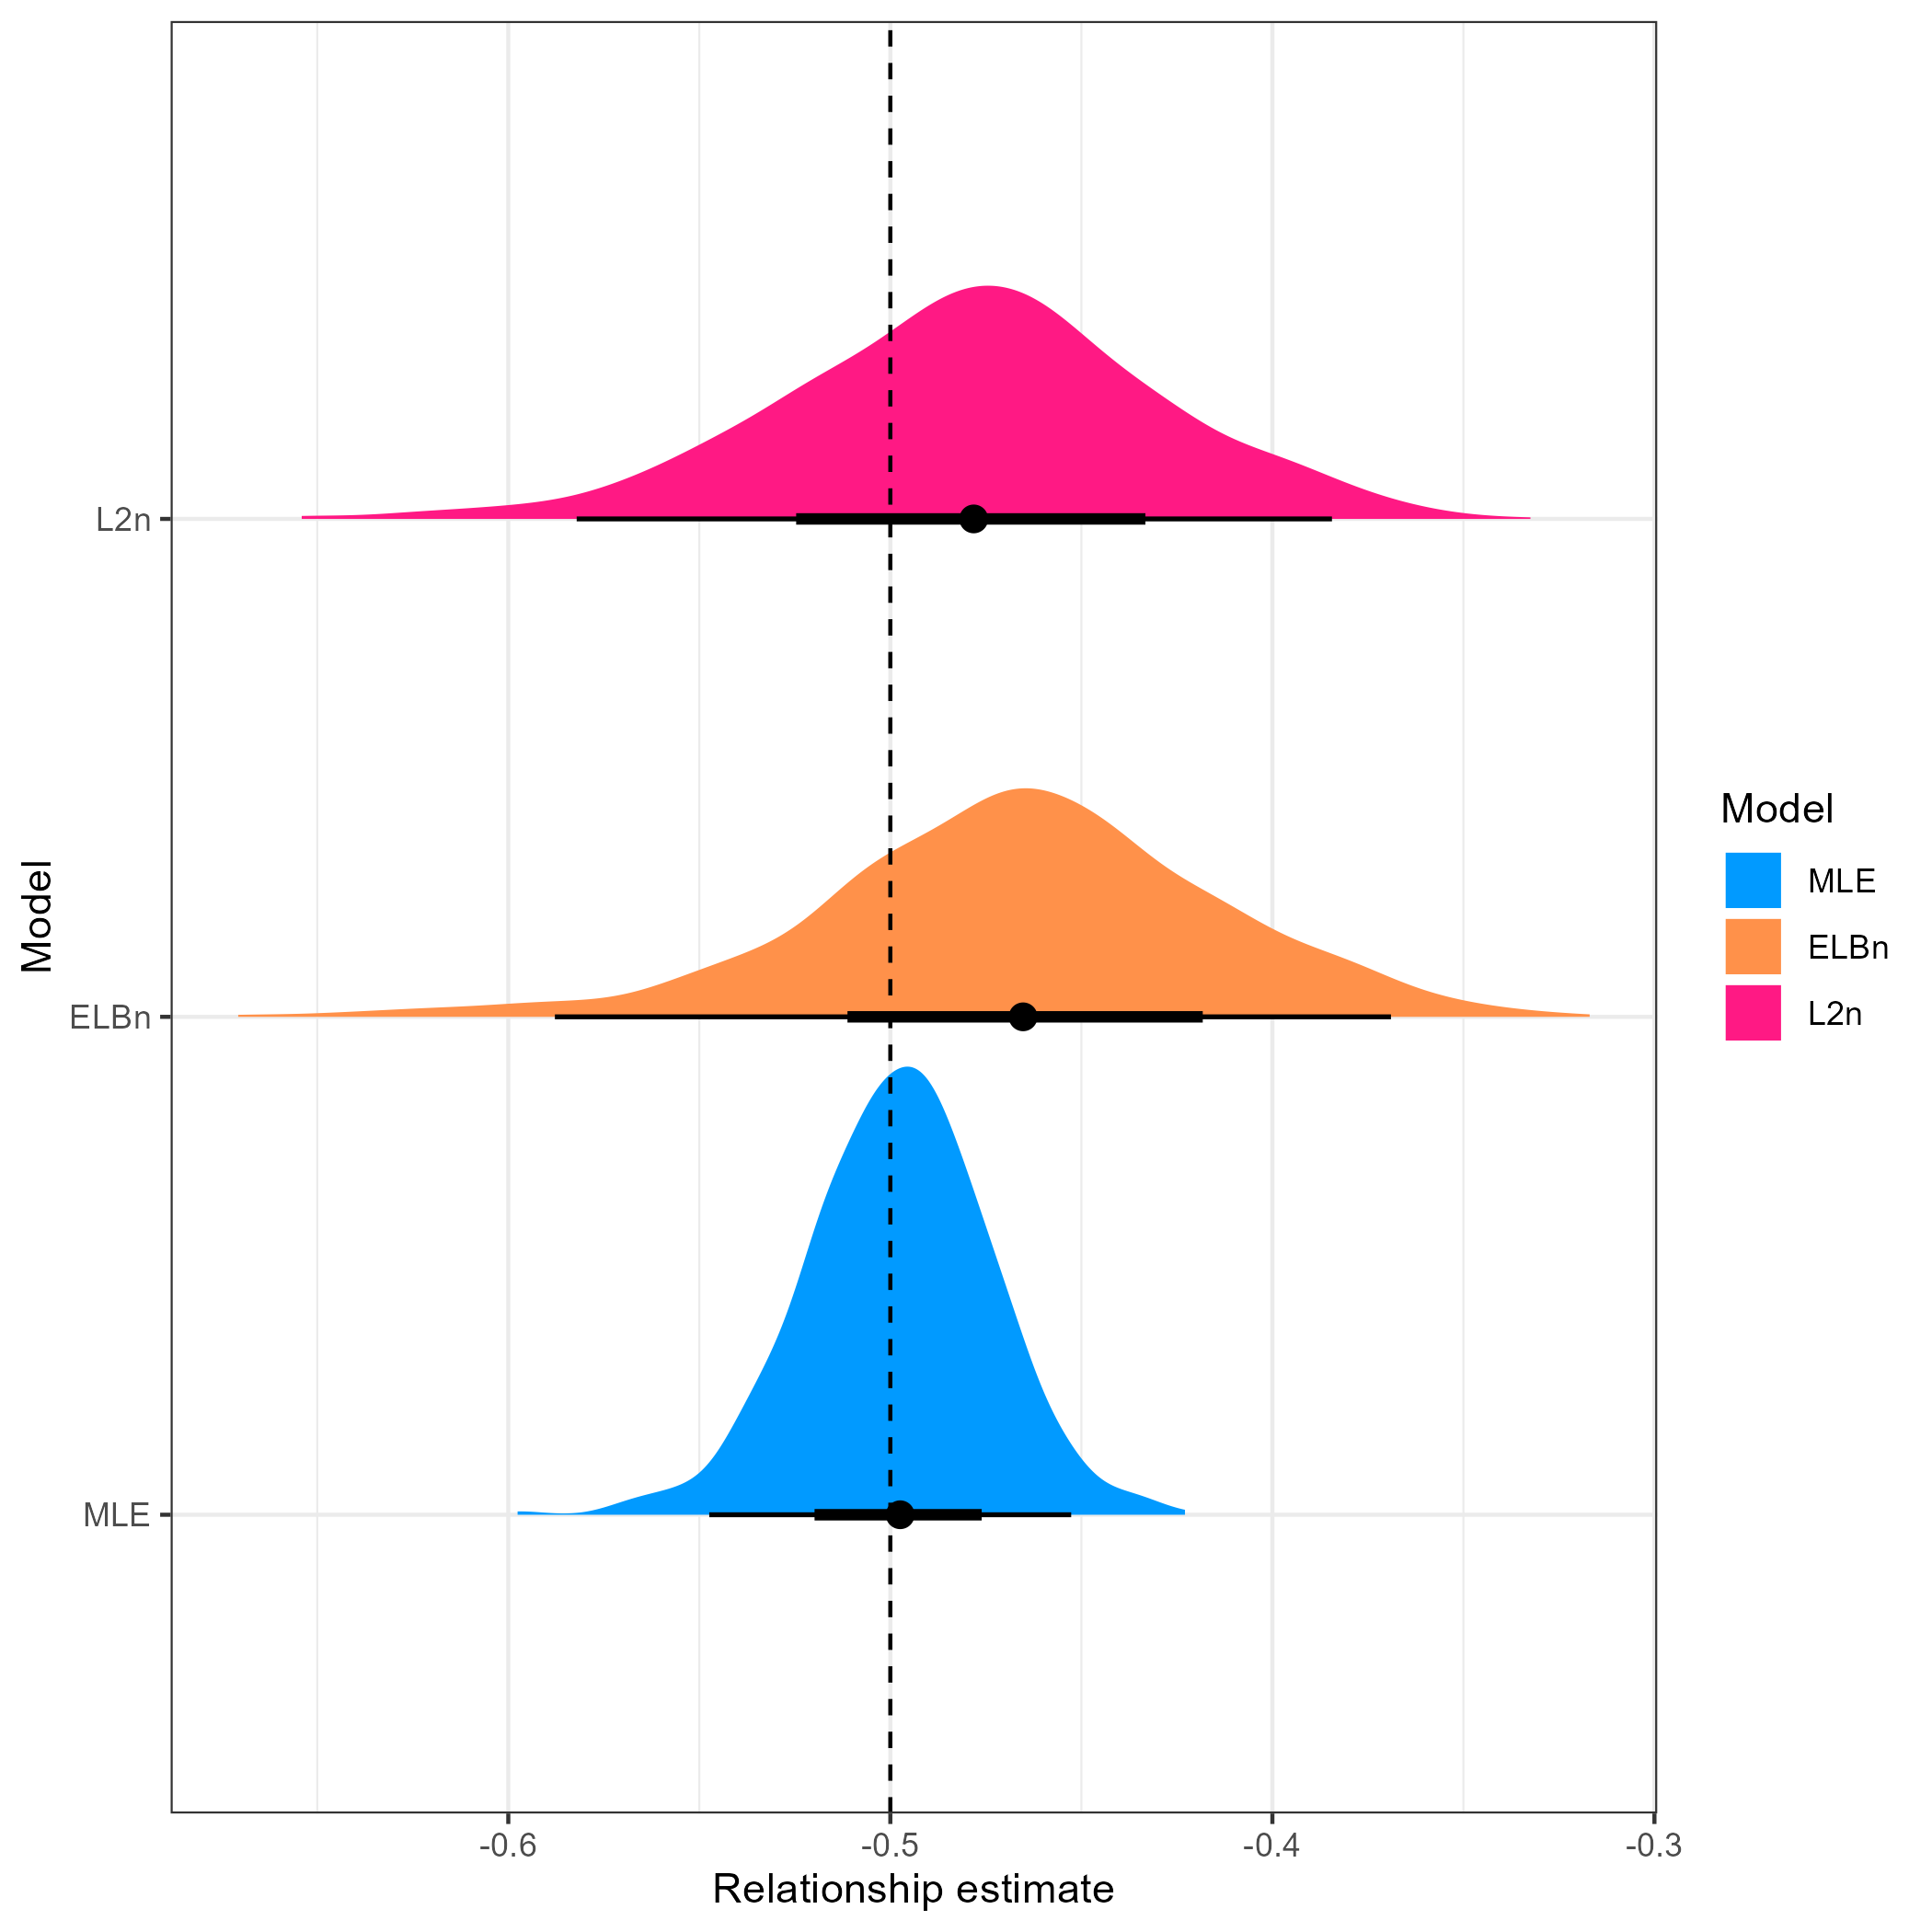
\includegraphics{figures/PLB_small_m_relationship_density.png}
\caption{Distribution of estimated relationship (\(\beta_1\))
coefficient's for five sites across a hypothetical gradient with known
value of 0.5. Range of body sizes is reduced and is from 1, to 100.}
\end{figure}

\newpage

\hypertarget{sample-size-n}{%
\subsection{\texorpdfstring{Sample size,
\(n\)}{Sample size, n}}\label{sample-size-n}}

The number of observations in our simulations may bias the results.
Therefore, we repeated the simulations described above, but varied the
sample size \(n\). We tested values of
\(n = 200, 500, 1000, 5000, 10 000\). Results of this analysis are
presented in the Supplemental Information.

\begin{figure}
\centering
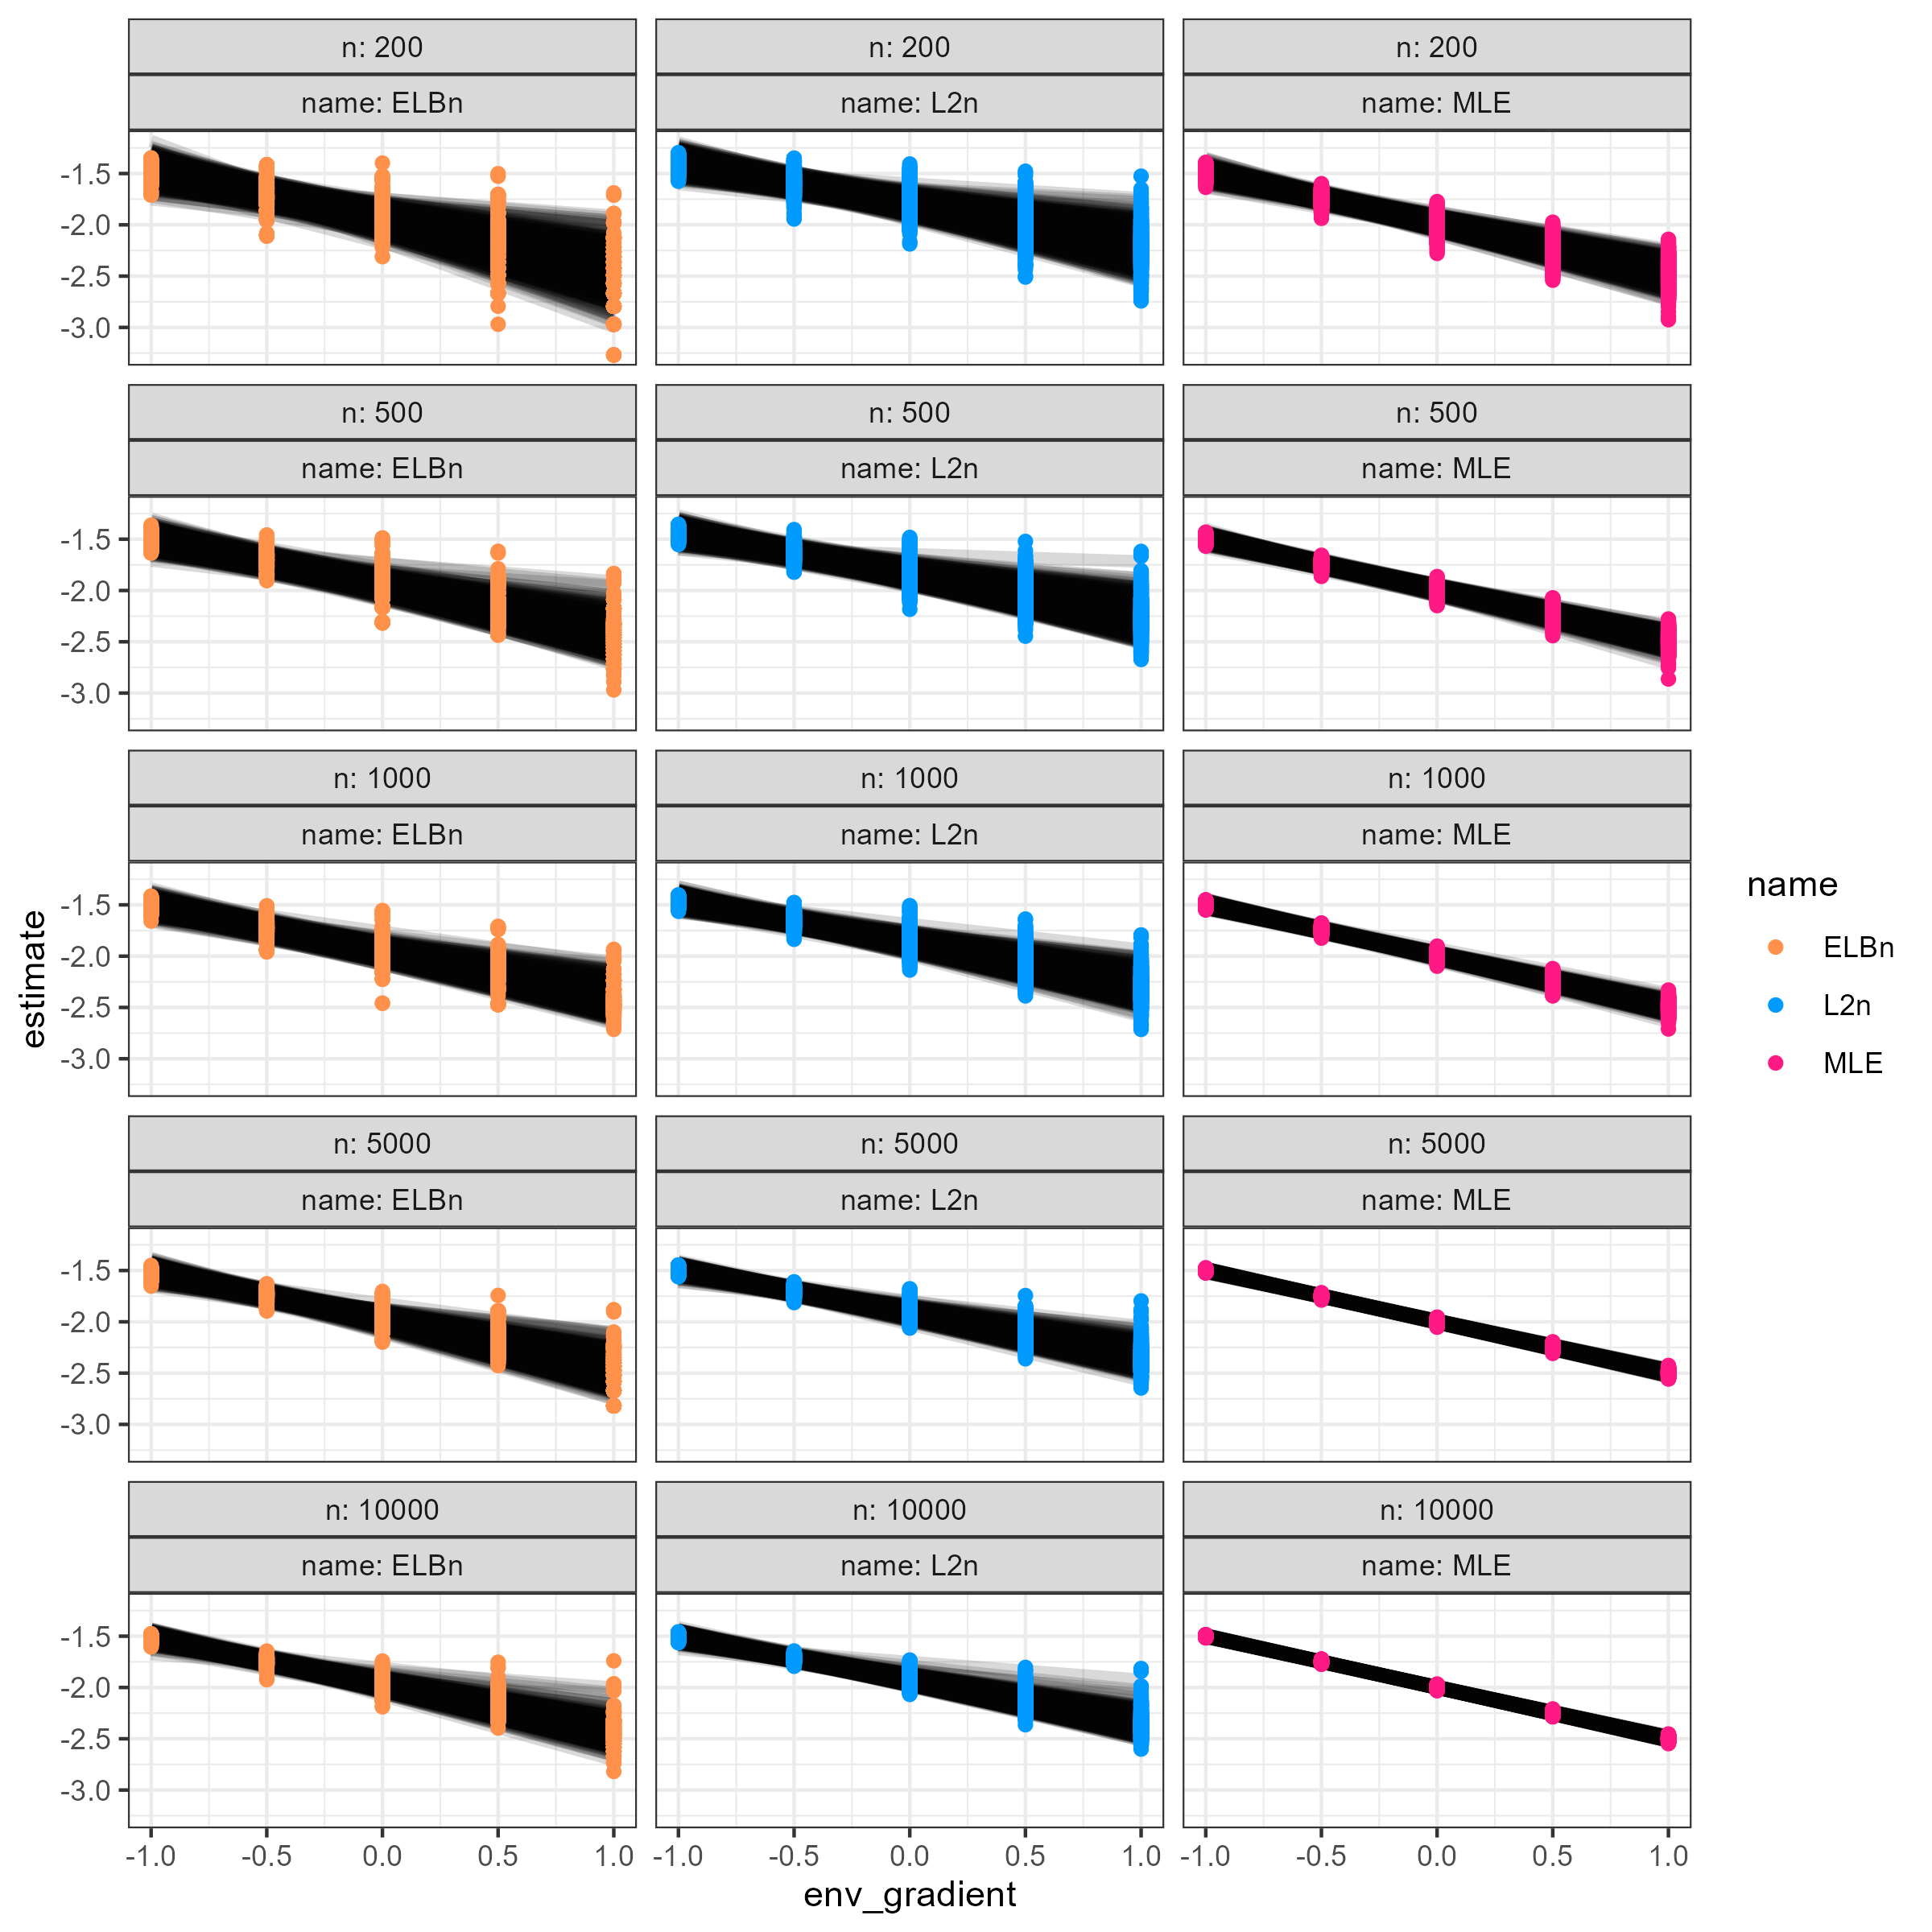
\includegraphics{figures/n_vary_main.png}
\caption{Individual regression estimates across the hypothetical
gradient based on sample size (rows) and methodology used (columns).
(match this figure to ``new'' style if we like that better)}
\end{figure}

\begin{figure}
\centering
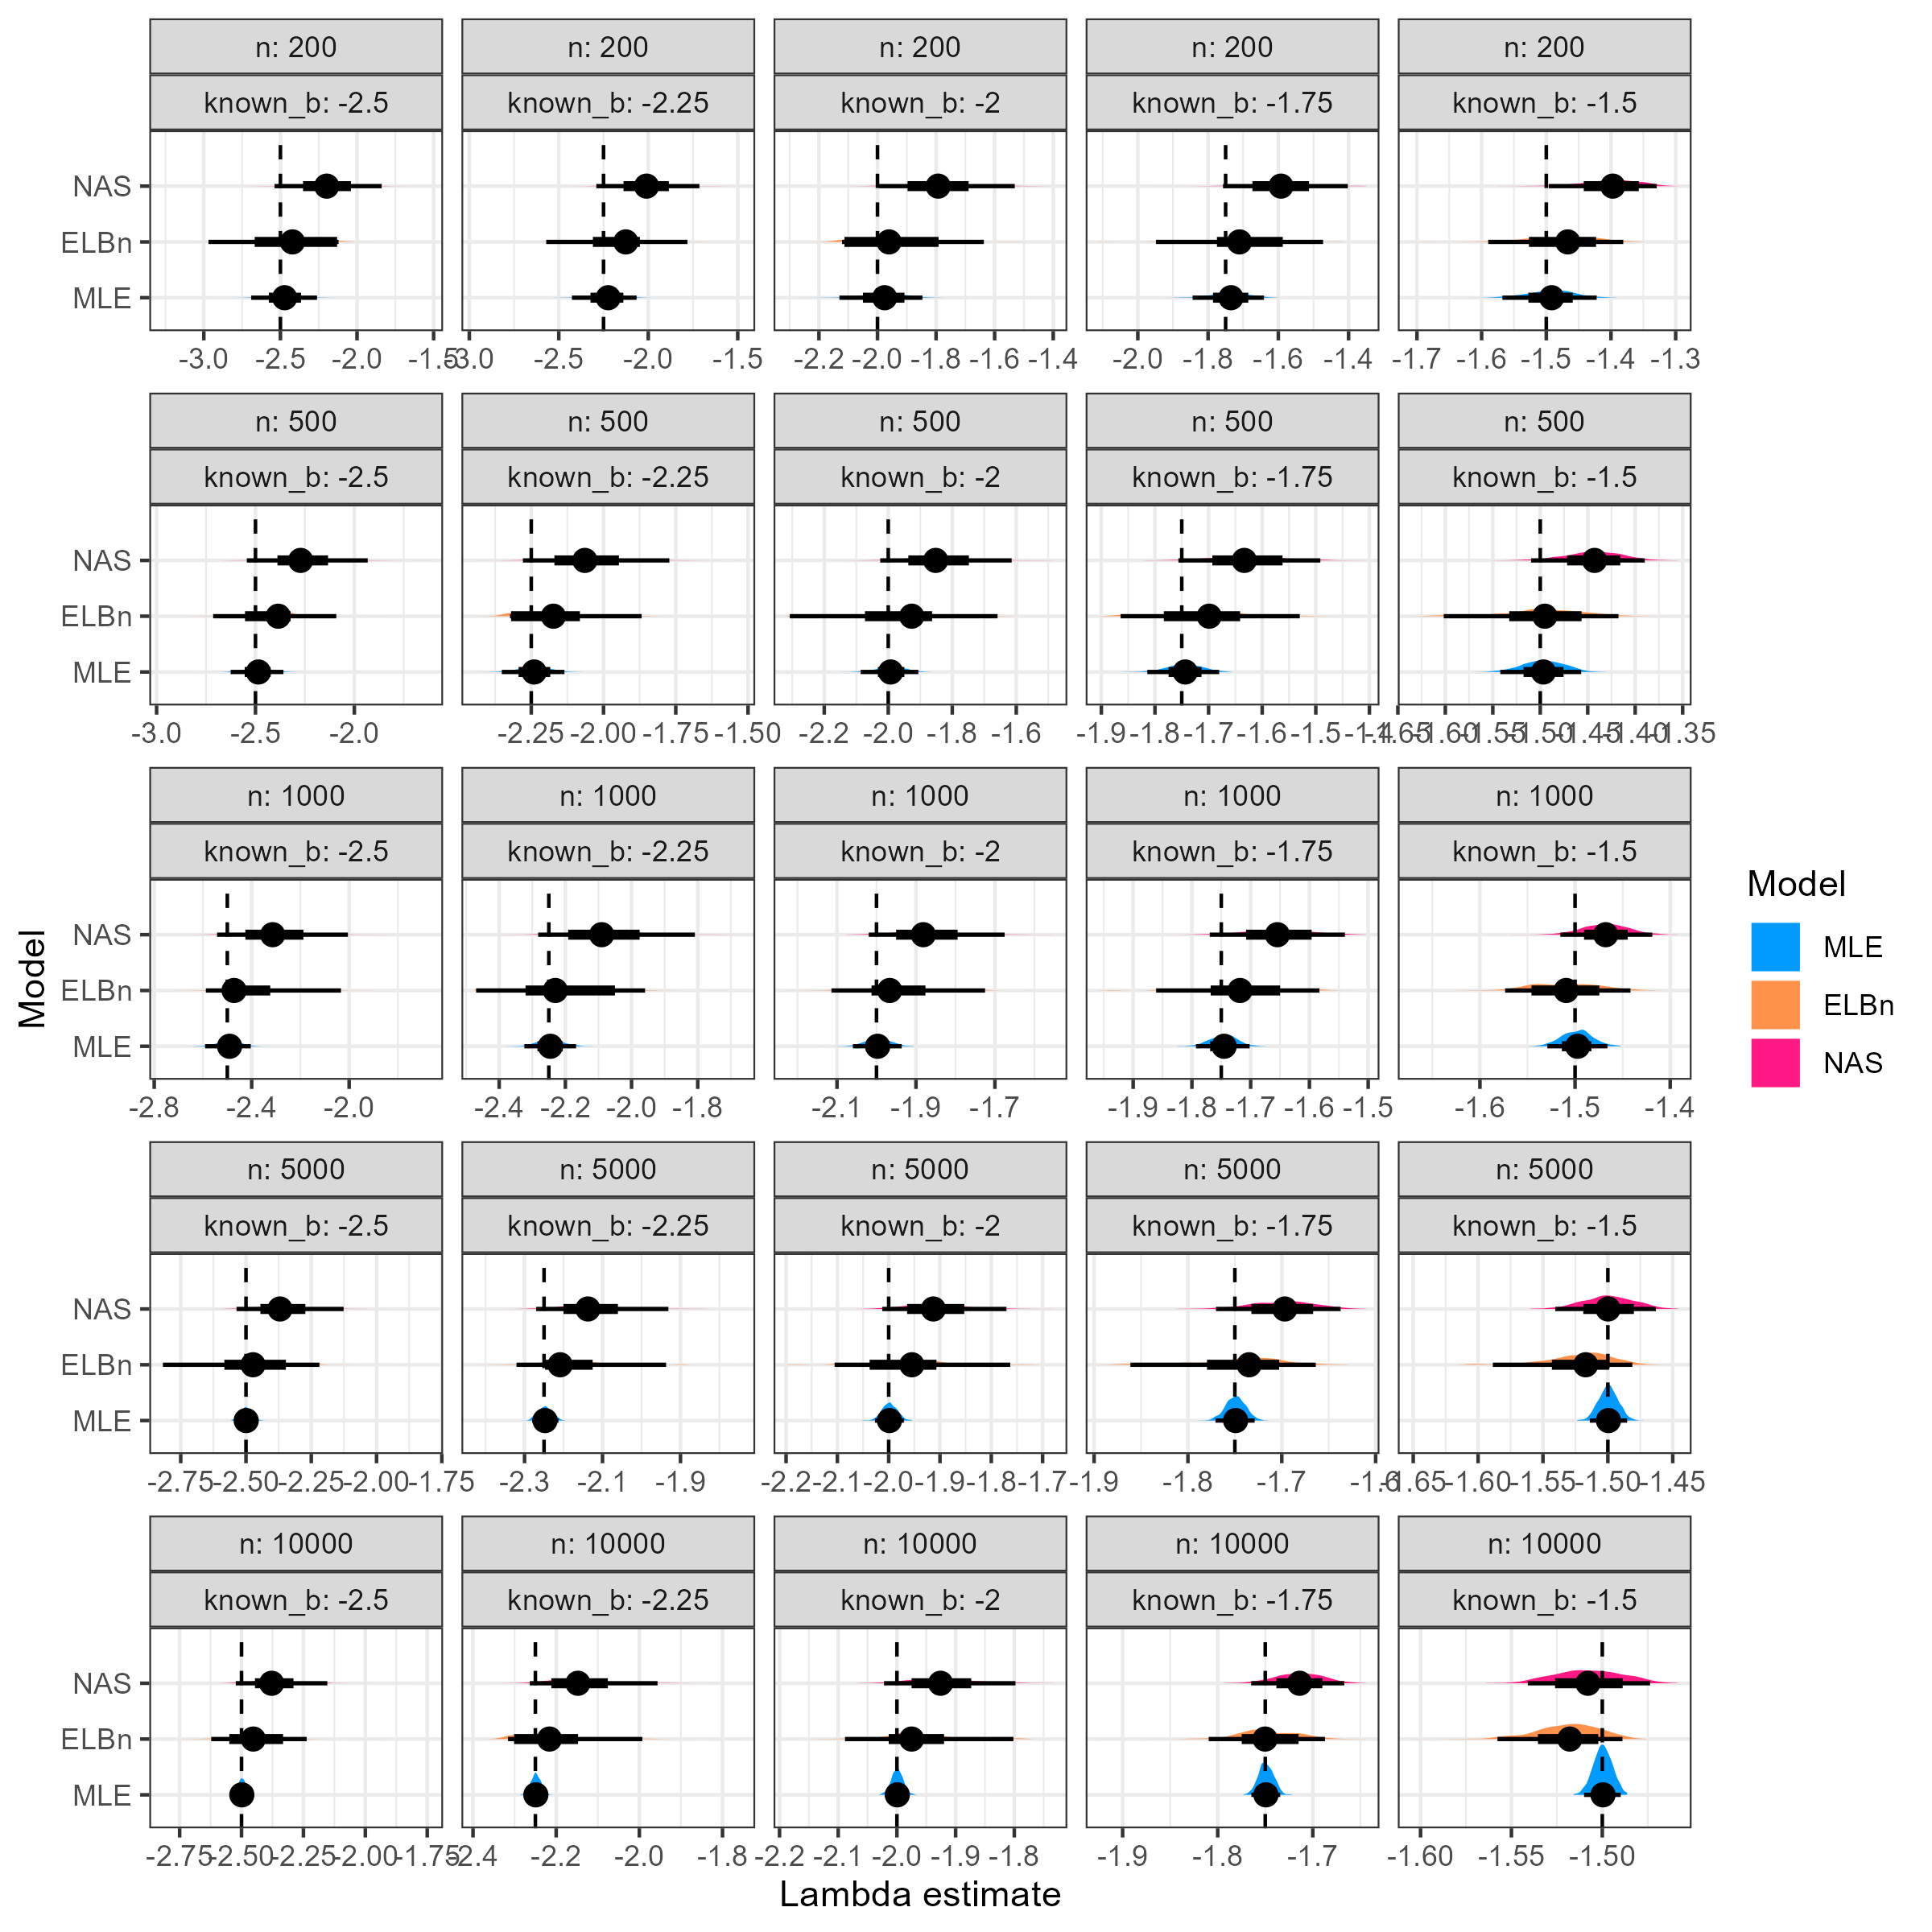
\includegraphics{figures/n_vary_est_b.png}
\caption{Distribution of size spectra parameter estimates. Vertical line
is the known parameter (dashed line) wich describes the bounded power
law distribution from which the body size estimates were sampled. As n
increases (top to bottom) and \(\lambda\) increases (left to right), the
accuracy of the estimate improves across all methods.}
\end{figure}

\newpage

\begin{figure}
\centering
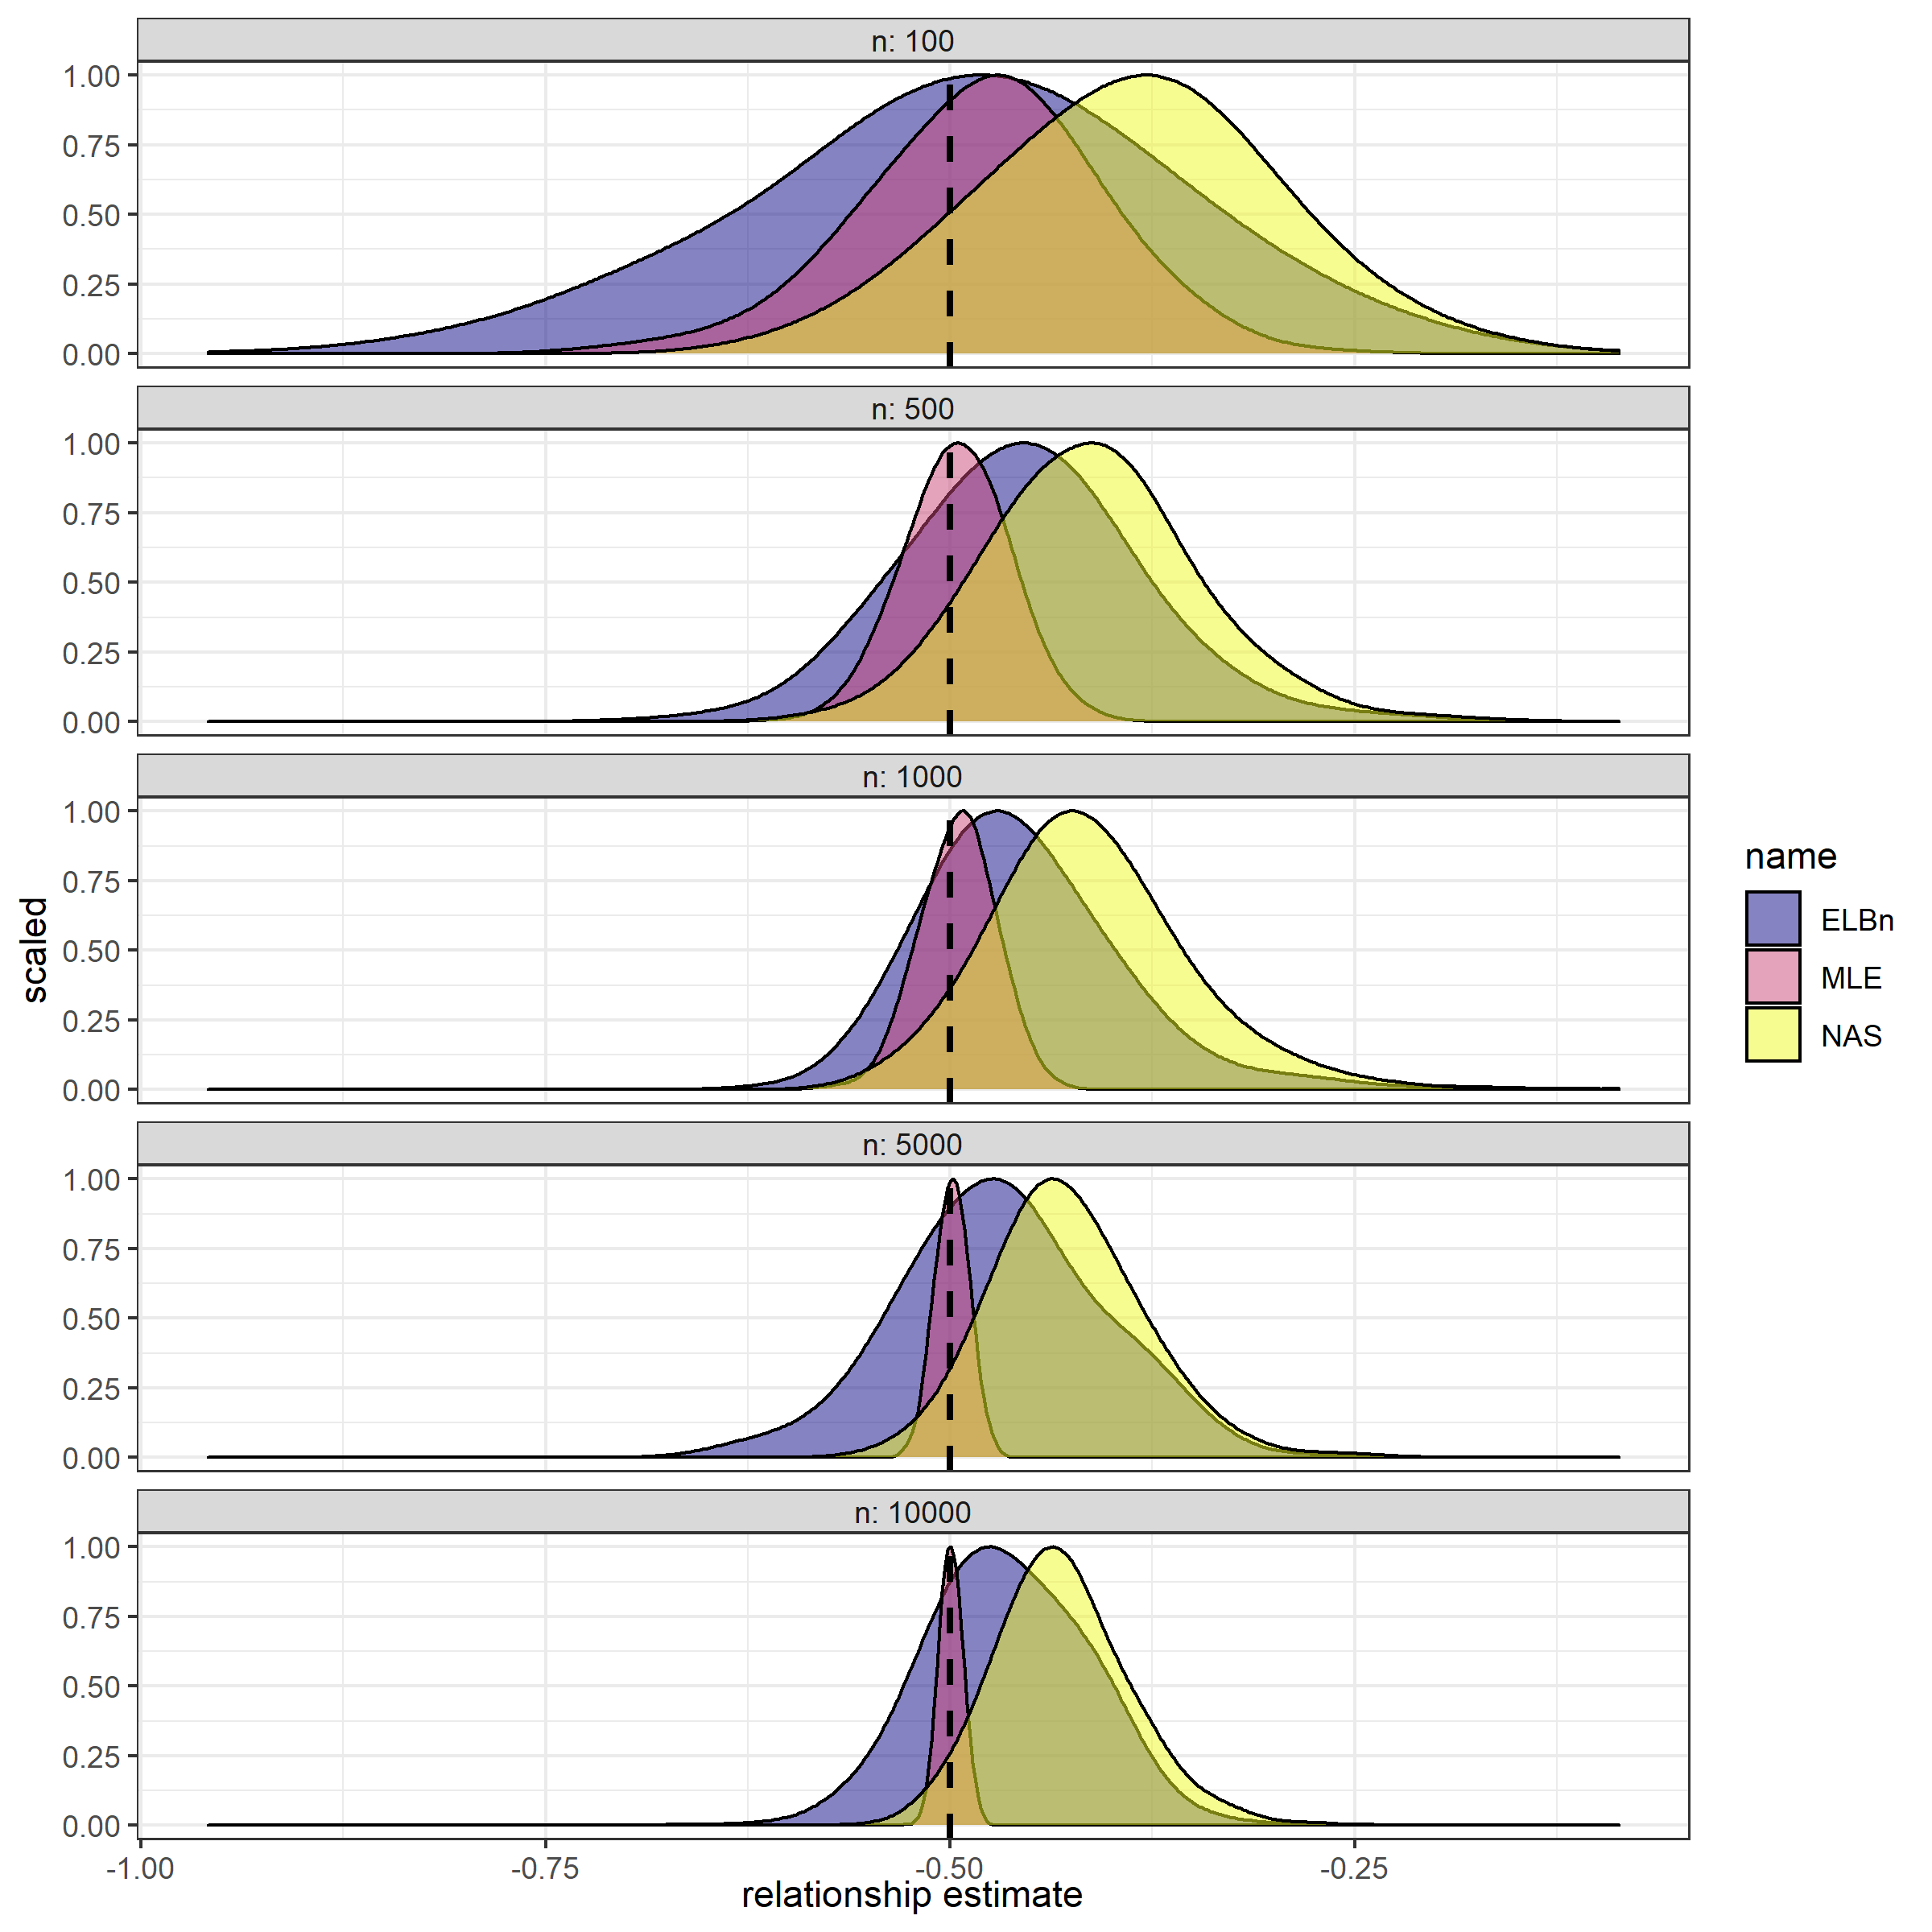
\includegraphics{figures/n_vary_relationship_density.png}
\caption{Distribtuion of the relationship coefficients with varying
sample size}
\end{figure}

\newpage

\hypertarget{range-of-body-sizes-1-to-100}{%
\subsubsection{Range of body sizes = 1 to
100}\label{range-of-body-sizes-1-to-100}}

\begin{figure}
\centering
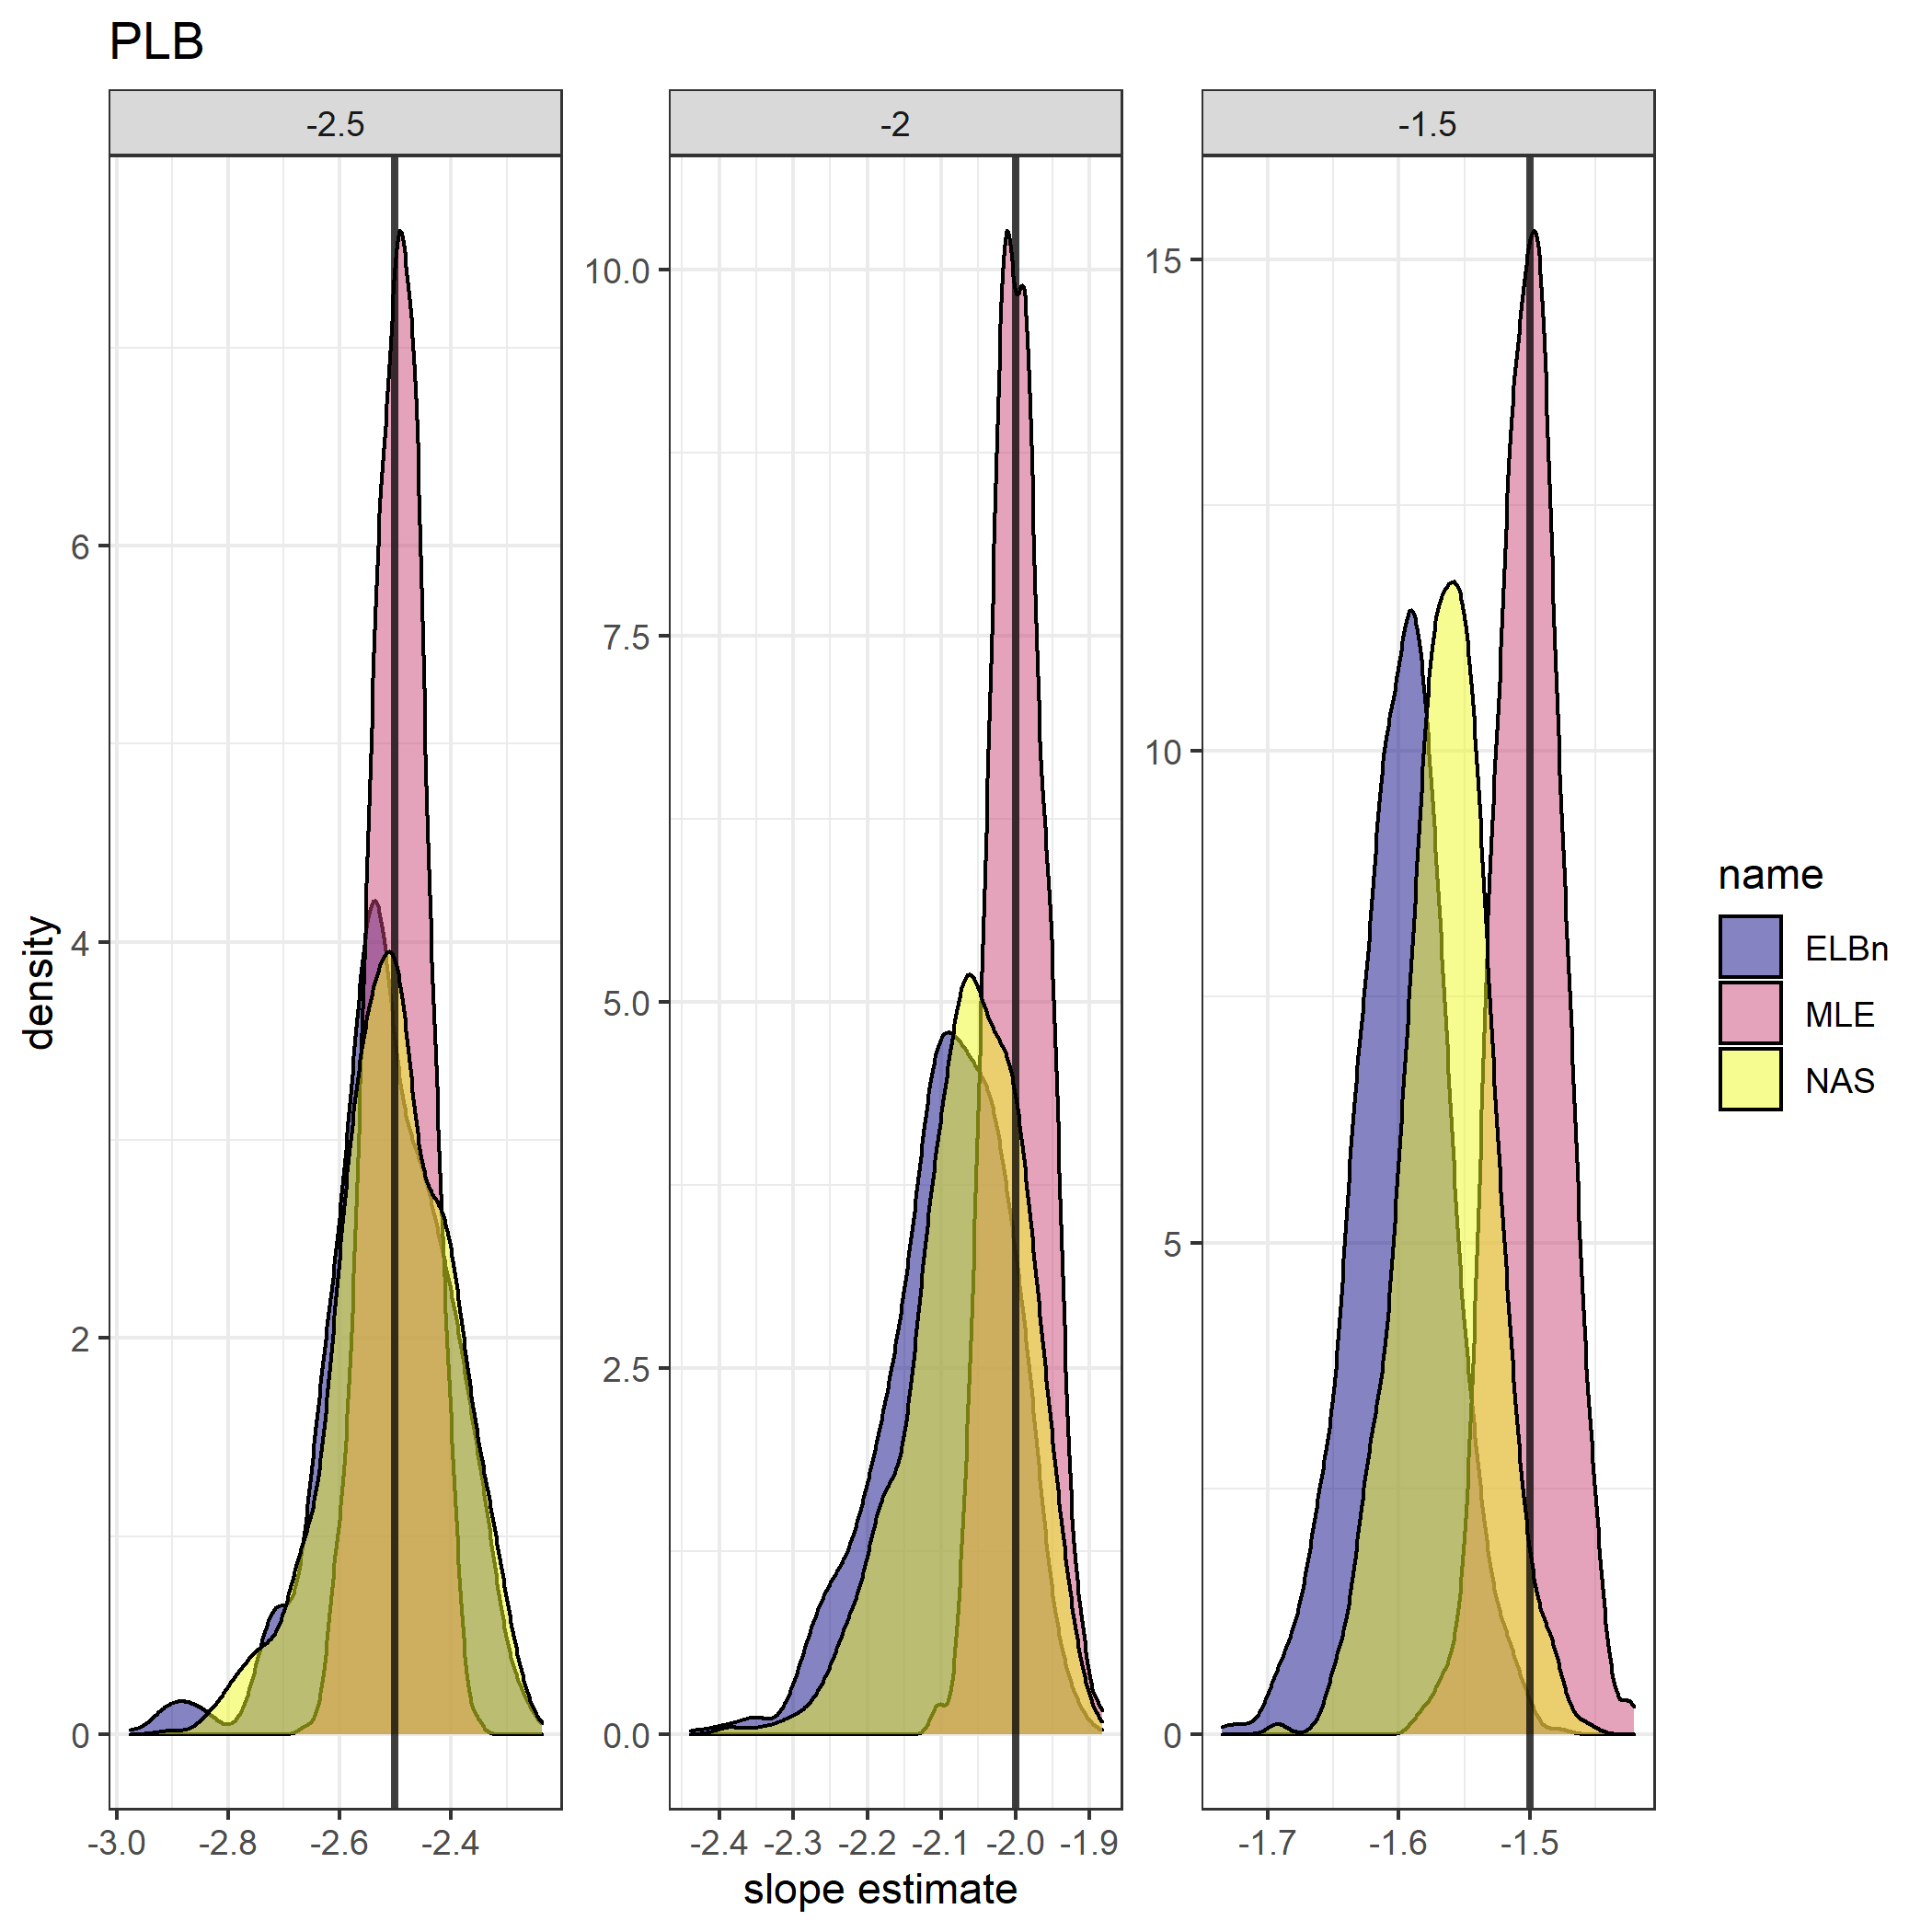
\includegraphics{figures/PLB_small_m_est_b_density.png}
\caption{Distribution of estimated \$\textbackslash lambda\$ coefficient
for five sites across a hypothetical gradient with known values(dashed
line). Range of body sizes is smaller than main anaysis and ranges from
1, to 100.}
\end{figure}

\newpage

\begin{figure}
\centering
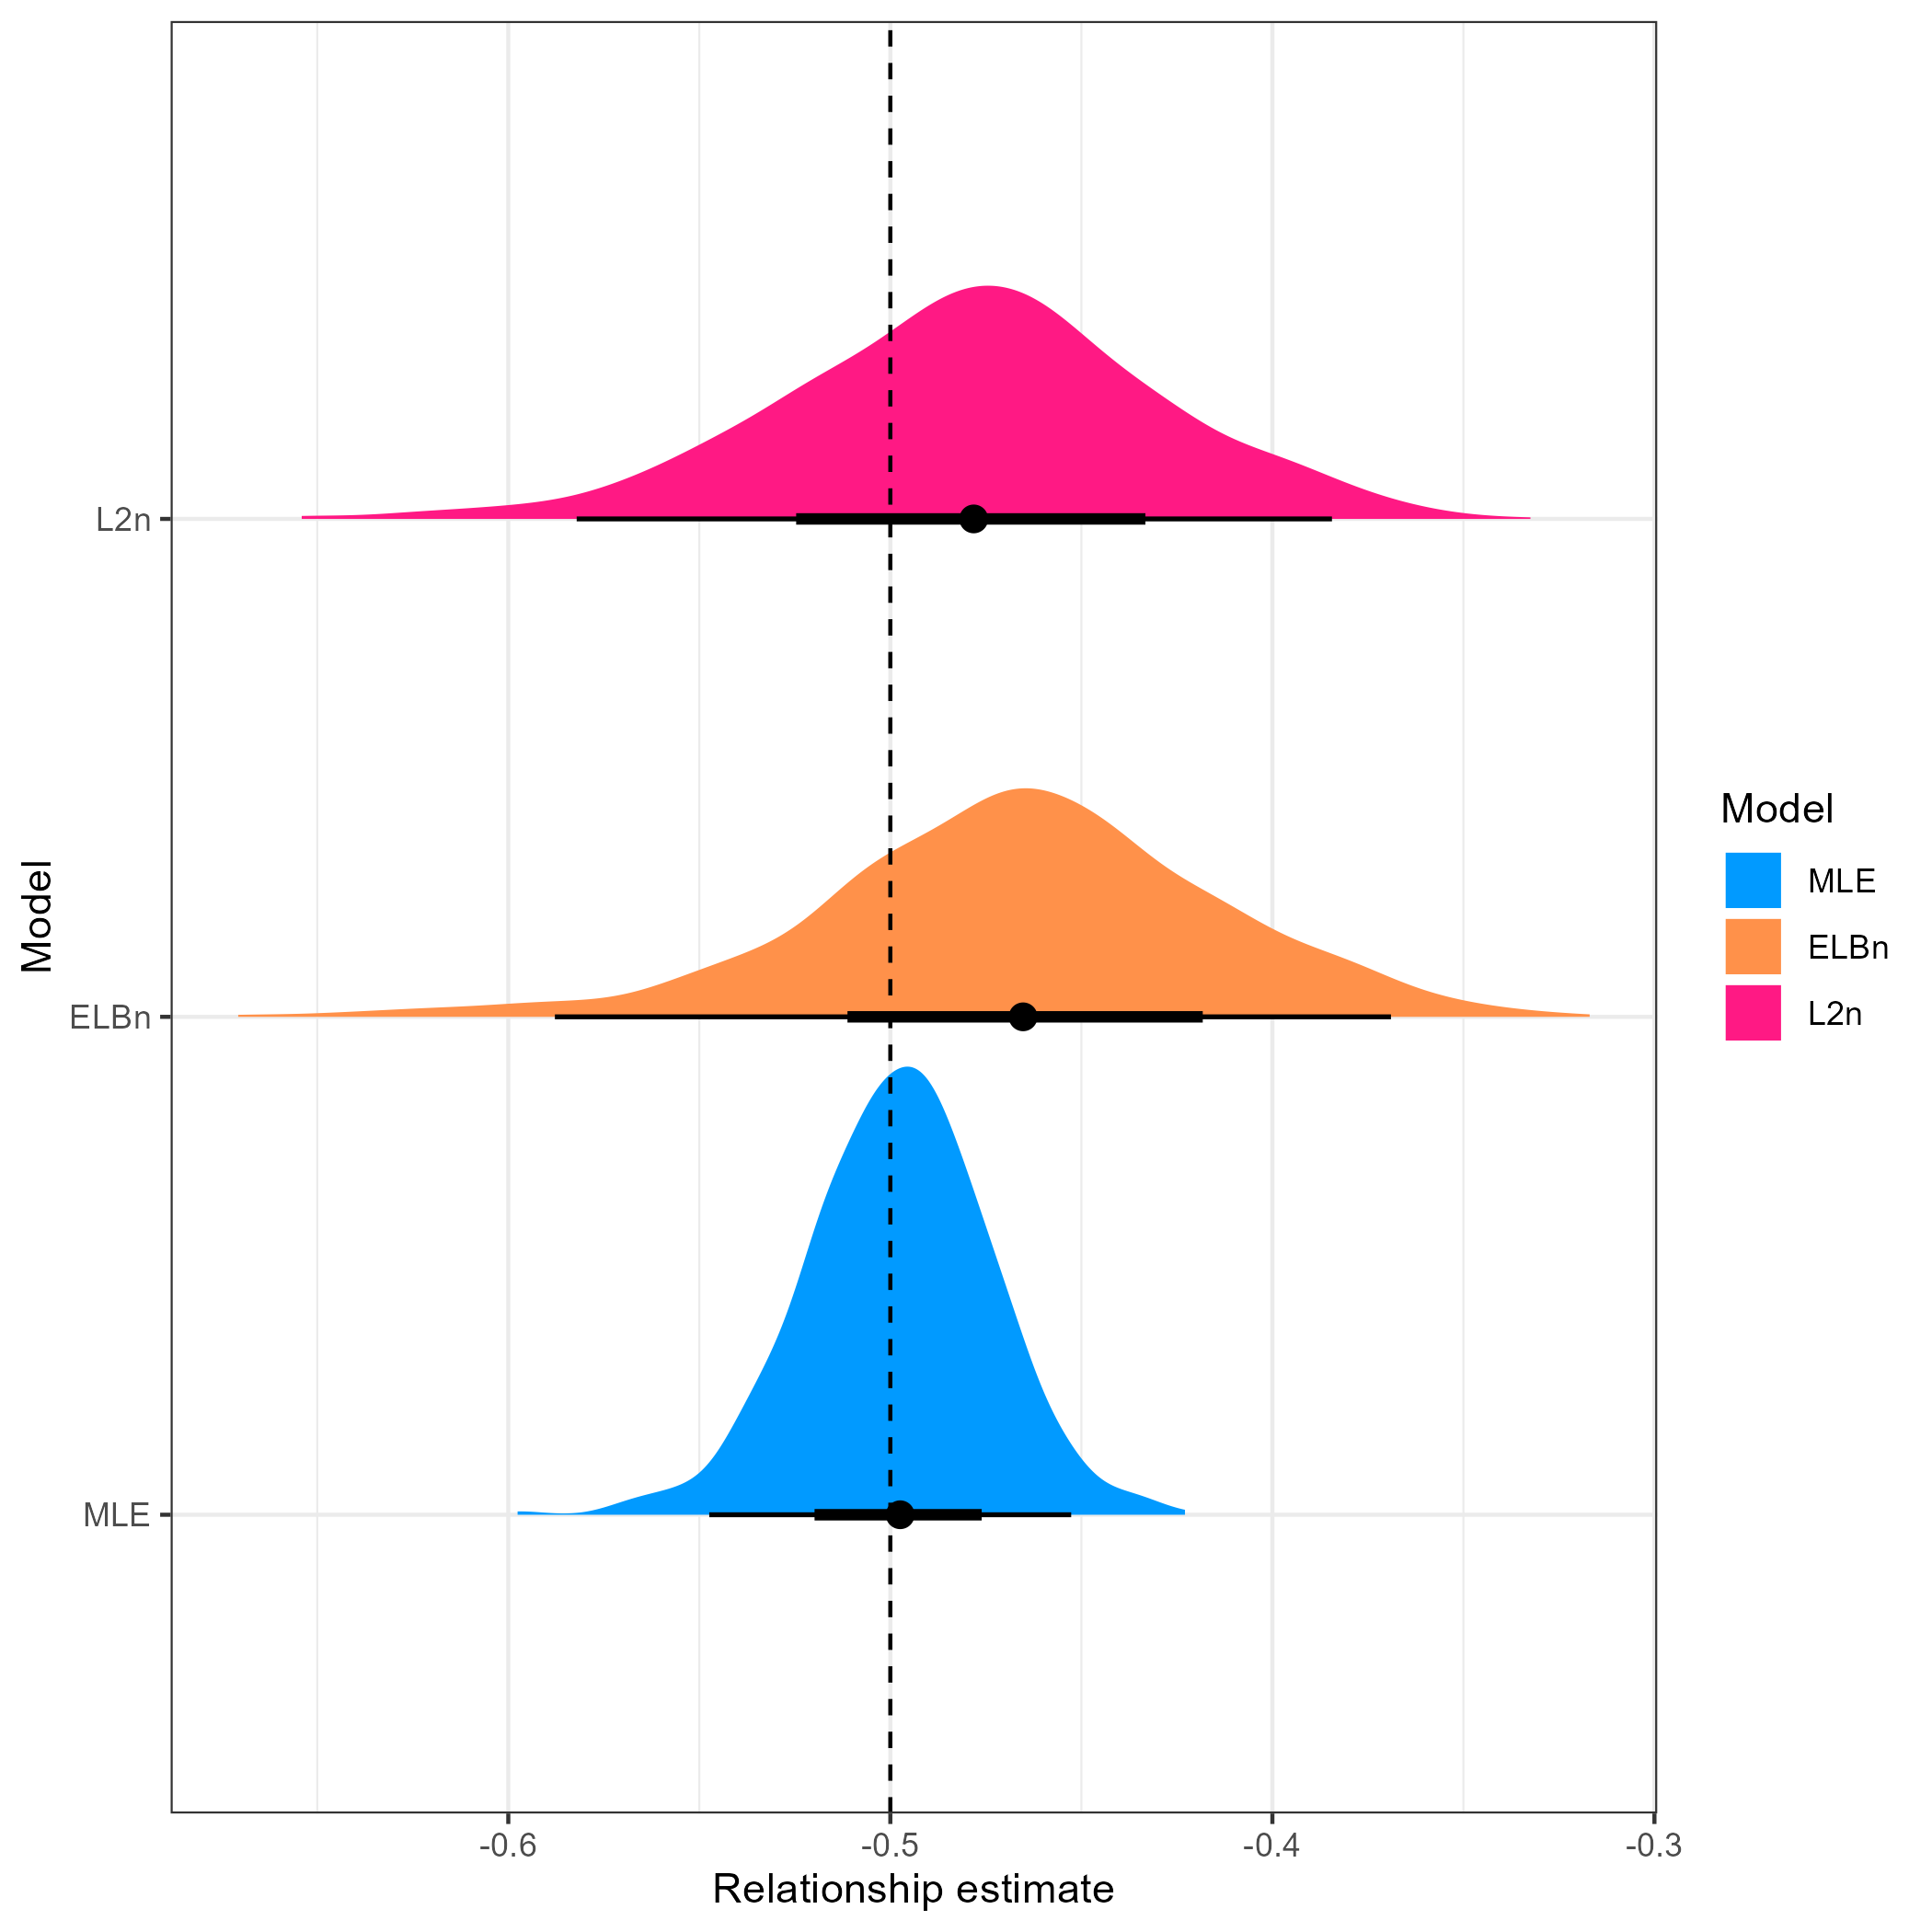
\includegraphics{figures/PLB_small_m_relationship_density.png}
\caption{Relationship estimate}
\end{figure}

\hypertarget{comparison-with-other-published-estimates}{%
\section{Comparison with other published
estimates}\label{comparison-with-other-published-estimates}}

SI Table. This table shows published estimates of the variation in size
spectra slopes (or exponents) in empirical studies. It is unclear how to
directly compare estimates of the slope with different methods.However,
the published estimates here range from \textasciitilde0.1 to 0.2 across
the gradients studied. For comparison, the 2.5-95\% quantiles around the
relationship estimate for the MLE method were \textasciitilde0.1,
whereas for the ELBn and NAS method they were \textasciitilde0.25 and
\textasciitilde0.2, respectively. b\_diff is the change in estimate
(b-low - b-min). System refers to stream communities or mesocosm
experiments. Method: MLE = maximum likelihod estimate, ELB = equal
logarthmic binning, the number before indicates the number of bins used.
The normalization process shifts the estimates by an absolute value of
1.0. Hence, direct comparison the relative change in normalized and
non-normalized studies should not introduce any bias. The O'Gorman et
al.~2017 study used average species size and abundance (Local Size
Density Relationship, \emph{sensu} White et al.~2007) as opposed to
individual size distribution. These methods are related, but it is
unclear how to directly compare estimates from each method.

\begin{longtable}[]{@{}lrrlrrlll@{}}
\toprule
\begin{minipage}[b]{(\columnwidth - 8\tabcolsep) * \real{0.23}}\raggedright
Citation\strut
\end{minipage} &
\begin{minipage}[b]{(\columnwidth - 8\tabcolsep) * \real{0.11}}\raggedleft
\(\beta_1\) Difference\strut
\end{minipage} &
\begin{minipage}[b]{(\columnwidth - 8\tabcolsep) * \real{0.03}}\raggedleft
Error\strut
\end{minipage} &
\begin{minipage}[b]{(\columnwidth - 8\tabcolsep) * \real{0.06}}\raggedright
Error Type\strut
\end{minipage} &
\begin{minipage}[b]{(\columnwidth - 8\tabcolsep) * \real{0.08}}\raggedleft
\(\beta_{low}\)\strut
\end{minipage} &
\begin{minipage}[b]{(\columnwidth - 8\tabcolsep) * \real{0.08}}\raggedleft
\(\beta_{high}\)\strut
\end{minipage} &
\begin{minipage}[b]{(\columnwidth - 8\tabcolsep) * \real{0.07}}\raggedright
System\strut
\end{minipage} &
\begin{minipage}[b]{(\columnwidth - 8\tabcolsep) * \real{0.06}}\raggedright
Driver\strut
\end{minipage} &
\begin{minipage}[b]{(\columnwidth - 8\tabcolsep) * \real{0.28}}\raggedright
Method\strut
\end{minipage}\tabularnewline
\midrule
\endhead
\begin{minipage}[t]{(\columnwidth - 8\tabcolsep) * \real{0.23}}\raggedright
Pomeranz et al.~2021\strut
\end{minipage} &
\begin{minipage}[t]{(\columnwidth - 8\tabcolsep) * \real{0.11}}\raggedleft
0.12\strut
\end{minipage} &
\begin{minipage}[t]{(\columnwidth - 8\tabcolsep) * \real{0.03}}\raggedleft
NA\strut
\end{minipage} &
\begin{minipage}[t]{(\columnwidth - 8\tabcolsep) * \real{0.06}}\raggedright
\strut
\end{minipage} &
\begin{minipage}[t]{(\columnwidth - 8\tabcolsep) * \real{0.08}}\raggedleft
-1.37\strut
\end{minipage} &
\begin{minipage}[t]{(\columnwidth - 8\tabcolsep) * \real{0.08}}\raggedleft
-1.25\strut
\end{minipage} &
\begin{minipage}[t]{(\columnwidth - 8\tabcolsep) * \real{0.07}}\raggedright
Streams\strut
\end{minipage} &
\begin{minipage}[t]{(\columnwidth - 8\tabcolsep) * \real{0.06}}\raggedright
Temperature\strut
\end{minipage} &
\begin{minipage}[t]{(\columnwidth - 8\tabcolsep) * \real{0.28}}\raggedright
MLE\strut
\end{minipage}\tabularnewline
\begin{minipage}[t]{(\columnwidth - 8\tabcolsep) * \real{0.23}}\raggedright
Yvon Durocher et al.~2011 (Community)\strut
\end{minipage} &
\begin{minipage}[t]{(\columnwidth - 8\tabcolsep) * \real{0.11}}\raggedleft
0.13\strut
\end{minipage} &
\begin{minipage}[t]{(\columnwidth - 8\tabcolsep) * \real{0.03}}\raggedleft
NA\strut
\end{minipage} &
\begin{minipage}[t]{(\columnwidth - 8\tabcolsep) * \real{0.06}}\raggedright
\strut
\end{minipage} &
\begin{minipage}[t]{(\columnwidth - 8\tabcolsep) * \real{0.08}}\raggedleft
-0.79\strut
\end{minipage} &
\begin{minipage}[t]{(\columnwidth - 8\tabcolsep) * \real{0.08}}\raggedleft
-0.92\strut
\end{minipage} &
\begin{minipage}[t]{(\columnwidth - 8\tabcolsep) * \real{0.07}}\raggedright
FW mesocosms\strut
\end{minipage} &
\begin{minipage}[t]{(\columnwidth - 8\tabcolsep) * \real{0.06}}\raggedright
Temperature\strut
\end{minipage} &
\begin{minipage}[t]{(\columnwidth - 8\tabcolsep) * \real{0.28}}\raggedright
10 ELB, not normalized\strut
\end{minipage}\tabularnewline
\begin{minipage}[t]{(\columnwidth - 8\tabcolsep) * \real{0.23}}\raggedright
Dossena et al.~2012 (October)\strut
\end{minipage} &
\begin{minipage}[t]{(\columnwidth - 8\tabcolsep) * \real{0.11}}\raggedleft
0.14\strut
\end{minipage} &
\begin{minipage}[t]{(\columnwidth - 8\tabcolsep) * \real{0.03}}\raggedleft
0.070\strut
\end{minipage} &
\begin{minipage}[t]{(\columnwidth - 8\tabcolsep) * \real{0.06}}\raggedright
se\strut
\end{minipage} &
\begin{minipage}[t]{(\columnwidth - 8\tabcolsep) * \real{0.08}}\raggedleft
NA\strut
\end{minipage} &
\begin{minipage}[t]{(\columnwidth - 8\tabcolsep) * \real{0.08}}\raggedleft
NA\strut
\end{minipage} &
\begin{minipage}[t]{(\columnwidth - 8\tabcolsep) * \real{0.07}}\raggedright
FW mesocosms\strut
\end{minipage} &
\begin{minipage}[t]{(\columnwidth - 8\tabcolsep) * \real{0.06}}\raggedright
Temperature\strut
\end{minipage} &
\begin{minipage}[t]{(\columnwidth - 8\tabcolsep) * \real{0.28}}\raggedright
6 ELB, not normalized\strut
\end{minipage}\tabularnewline
\begin{minipage}[t]{(\columnwidth - 8\tabcolsep) * \real{0.23}}\raggedright
O'Gorman et al.~2017\strut
\end{minipage} &
\begin{minipage}[t]{(\columnwidth - 8\tabcolsep) * \real{0.11}}\raggedleft
0.15\strut
\end{minipage} &
\begin{minipage}[t]{(\columnwidth - 8\tabcolsep) * \real{0.03}}\raggedleft
NA\strut
\end{minipage} &
\begin{minipage}[t]{(\columnwidth - 8\tabcolsep) * \real{0.06}}\raggedright
\strut
\end{minipage} &
\begin{minipage}[t]{(\columnwidth - 8\tabcolsep) * \real{0.08}}\raggedleft
-0.85\strut
\end{minipage} &
\begin{minipage}[t]{(\columnwidth - 8\tabcolsep) * \real{0.08}}\raggedleft
-0.70\strut
\end{minipage} &
\begin{minipage}[t]{(\columnwidth - 8\tabcolsep) * \real{0.07}}\raggedright
Streams\strut
\end{minipage} &
\begin{minipage}[t]{(\columnwidth - 8\tabcolsep) * \real{0.06}}\raggedright
Temperature\strut
\end{minipage} &
\begin{minipage}[t]{(\columnwidth - 8\tabcolsep) * \real{0.28}}\raggedright
ln (mean species abundance) \textasciitilde{} ln(mean species
mass)\strut
\end{minipage}\tabularnewline
\begin{minipage}[t]{(\columnwidth - 8\tabcolsep) * \real{0.23}}\raggedright
Martinez et al.~2016\strut
\end{minipage} &
\begin{minipage}[t]{(\columnwidth - 8\tabcolsep) * \real{0.11}}\raggedleft
0.15\strut
\end{minipage} &
\begin{minipage}[t]{(\columnwidth - 8\tabcolsep) * \real{0.03}}\raggedleft
NA\strut
\end{minipage} &
\begin{minipage}[t]{(\columnwidth - 8\tabcolsep) * \real{0.06}}\raggedright
\strut
\end{minipage} &
\begin{minipage}[t]{(\columnwidth - 8\tabcolsep) * \real{0.08}}\raggedleft
-1.11\strut
\end{minipage} &
\begin{minipage}[t]{(\columnwidth - 8\tabcolsep) * \real{0.08}}\raggedleft
-0.96\strut
\end{minipage} &
\begin{minipage}[t]{(\columnwidth - 8\tabcolsep) * \real{0.07}}\raggedright
Streams\strut
\end{minipage} &
\begin{minipage}[t]{(\columnwidth - 8\tabcolsep) * \real{0.06}}\raggedright
Land Use\strut
\end{minipage} &
\begin{minipage}[t]{(\columnwidth - 8\tabcolsep) * \real{0.28}}\raggedright
6 ELB, not normalized\strut
\end{minipage}\tabularnewline
\begin{minipage}[t]{(\columnwidth - 8\tabcolsep) * \real{0.23}}\raggedright
Yvon Durocher et al.~2011 (Phytoplankton)\strut
\end{minipage} &
\begin{minipage}[t]{(\columnwidth - 8\tabcolsep) * \real{0.11}}\raggedleft
0.19\strut
\end{minipage} &
\begin{minipage}[t]{(\columnwidth - 8\tabcolsep) * \real{0.03}}\raggedleft
NA\strut
\end{minipage} &
\begin{minipage}[t]{(\columnwidth - 8\tabcolsep) * \real{0.06}}\raggedright
\strut
\end{minipage} &
\begin{minipage}[t]{(\columnwidth - 8\tabcolsep) * \real{0.08}}\raggedleft
-0.46\strut
\end{minipage} &
\begin{minipage}[t]{(\columnwidth - 8\tabcolsep) * \real{0.08}}\raggedleft
-0.65\strut
\end{minipage} &
\begin{minipage}[t]{(\columnwidth - 8\tabcolsep) * \real{0.07}}\raggedright
FW mesocosms\strut
\end{minipage} &
\begin{minipage}[t]{(\columnwidth - 8\tabcolsep) * \real{0.06}}\raggedright
Temperature\strut
\end{minipage} &
\begin{minipage}[t]{(\columnwidth - 8\tabcolsep) * \real{0.28}}\raggedright
10 ELB, not normalized\strut
\end{minipage}\tabularnewline
\begin{minipage}[t]{(\columnwidth - 8\tabcolsep) * \real{0.23}}\raggedright
McGarvey and Kirk 2018\strut
\end{minipage} &
\begin{minipage}[t]{(\columnwidth - 8\tabcolsep) * \real{0.11}}\raggedleft
0.19\strut
\end{minipage} &
\begin{minipage}[t]{(\columnwidth - 8\tabcolsep) * \real{0.03}}\raggedleft
NA\strut
\end{minipage} &
\begin{minipage}[t]{(\columnwidth - 8\tabcolsep) * \real{0.06}}\raggedright
\strut
\end{minipage} &
\begin{minipage}[t]{(\columnwidth - 8\tabcolsep) * \real{0.08}}\raggedleft
-1.81\strut
\end{minipage} &
\begin{minipage}[t]{(\columnwidth - 8\tabcolsep) * \real{0.08}}\raggedleft
-1.62\strut
\end{minipage} &
\begin{minipage}[t]{(\columnwidth - 8\tabcolsep) * \real{0.07}}\raggedright
Streams\strut
\end{minipage} &
\begin{minipage}[t]{(\columnwidth - 8\tabcolsep) * \real{0.06}}\raggedright
Seasonality\strut
\end{minipage} &
\begin{minipage}[t]{(\columnwidth - 8\tabcolsep) * \real{0.28}}\raggedright
NAS, Log2 bins\strut
\end{minipage}\tabularnewline
\begin{minipage}[t]{(\columnwidth - 8\tabcolsep) * \real{0.23}}\raggedright
Dossena et al.~2012 (April)\strut
\end{minipage} &
\begin{minipage}[t]{(\columnwidth - 8\tabcolsep) * \real{0.11}}\raggedleft
0.21\strut
\end{minipage} &
\begin{minipage}[t]{(\columnwidth - 8\tabcolsep) * \real{0.03}}\raggedleft
0.064\strut
\end{minipage} &
\begin{minipage}[t]{(\columnwidth - 8\tabcolsep) * \real{0.06}}\raggedright
se\strut
\end{minipage} &
\begin{minipage}[t]{(\columnwidth - 8\tabcolsep) * \real{0.08}}\raggedleft
NA\strut
\end{minipage} &
\begin{minipage}[t]{(\columnwidth - 8\tabcolsep) * \real{0.08}}\raggedleft
NA\strut
\end{minipage} &
\begin{minipage}[t]{(\columnwidth - 8\tabcolsep) * \real{0.07}}\raggedright
FW mesocosms\strut
\end{minipage} &
\begin{minipage}[t]{(\columnwidth - 8\tabcolsep) * \real{0.06}}\raggedright
Temperature\strut
\end{minipage} &
\begin{minipage}[t]{(\columnwidth - 8\tabcolsep) * \real{0.28}}\raggedright
6 ELB, not normalized\strut
\end{minipage}\tabularnewline
\bottomrule
\end{longtable}

\end{document}
